% ============================================================================
% EEG-Based Depression Detection Using Deep Learning
% A Comprehensive Project Report
% ============================================================================

\documentclass[12pt,a4paper,oneside]{report}

% ============================================================================
% PACKAGES
% ============================================================================

% Page geometry - as per specifications
\usepackage[left=1.25in, right=0.75in, top=1in, bottom=1in]{geometry}

% Font settings (Times New Roman equivalent)
\usepackage{times}
\usepackage[T1]{fontenc}
\usepackage[utf8]{inputenc}

% Line spacing - 1.5 as specified
\usepackage{setspace}
\onehalfspacing

% Graphics and figures
\usepackage{graphicx}
\usepackage{float}
\usepackage{subcaption}
\usepackage[labelfont=bf]{caption}

% Tables
\usepackage{booktabs}
\usepackage{longtable}
\usepackage{multirow}
\usepackage{array}
\usepackage{tabularx}
\usepackage{ragged2e}

% Better table column types
\newcolumntype{L}[1]{>{\RaggedRight\arraybackslash}p{#1}}
\newcolumntype{C}[1]{>{\centering\arraybackslash}p{#1}}
\newcolumntype{R}[1]{>{\RaggedLeft\arraybackslash}p{#1}}

% Table row spacing
\renewcommand{\arraystretch}{1.2}

% Mathematics
\usepackage{amsmath}
\usepackage{amssymb}
\usepackage{amsfonts}

% Code listings
\usepackage{listings}
\usepackage{xcolor}

% Hyperlinks
\usepackage[hidelinks,colorlinks=false]{hyperref}

% Bibliography - numeric style with square brackets
\usepackage[numbers,square,sort&compress]{natbib}

% Algorithms
\usepackage{algorithm}
\usepackage{algorithmic}

% Chapter/Section formatting
\usepackage{titlesec}

% For list of abbreviations
\usepackage{nomencl}
\makenomenclature

% For better enumeration
\usepackage{enumitem}

% ============================================================================
% FORMATTING CONFIGURATION
% ============================================================================

% Chapter title: 14pt, bold, CAPS
\titleformat{\chapter}[display]
  {\normalfont\fontsize{14}{16}\bfseries}
  {\MakeUppercase{\chaptertitlename}\ \thechapter}{20pt}
  {\fontsize{14}{16}\bfseries\MakeUppercase}
\titlespacing*{\chapter}{0pt}{-20pt}{20pt}

% Section title: 13pt, bold, CAPS
\titleformat{\section}
  {\normalfont\fontsize{13}{15}\bfseries}
  {\thesection}{1em}{\MakeUppercase}

% Subsection title: 13pt, bold, Title Case
\titleformat{\subsection}
  {\normalfont\fontsize{13}{15}\bfseries}
  {\thesubsection}{1em}{}

% Subsubsection title: 12pt, bold
\titleformat{\subsubsection}
  {\normalfont\fontsize{12}{14}\bfseries}
  {\thesubsubsection}{1em}{}

% Figure/Table numbering as X.Y
\usepackage{chngcntr}
\counterwithin{figure}{chapter}
\counterwithin{table}{chapter}

% Custom figure and table naming
\renewcommand{\figurename}{Fig}
\renewcommand{\tablename}{Table}

% Caption formatting - 10pt, title case
\captionsetup{font=small,labelfont=bf,format=plain}
\captionsetup[figure]{position=below}
\captionsetup[table]{position=above}

% Code listing style
\definecolor{codegreen}{rgb}{0,0.6,0}
\definecolor{codegray}{rgb}{0.5,0.5,0.5}
\definecolor{codepurple}{rgb}{0.58,0,0.82}
\definecolor{backcolour}{rgb}{0.95,0.95,0.92}

\lstdefinestyle{pythonstyle}{
    backgroundcolor=\color{backcolour},
    commentstyle=\color{codegreen},
    keywordstyle=\color{magenta},
    numberstyle=\tiny\color{codegray},
    stringstyle=\color{codepurple},
    basicstyle=\ttfamily\footnotesize,
    breakatwhitespace=false,
    breaklines=true,
    captionpos=b,
    keepspaces=true,
    numbers=left,
    numbersep=5pt,
    showspaces=false,
    showstringspaces=false,
    showtabs=false,
    tabsize=2,
    language=Python
}
\lstset{style=pythonstyle}

% Page numbering at bottom center
\pagestyle{plain}

% ============================================================================
% DOCUMENT CONTENT
% ============================================================================

\begin{document}

% ----------------------------------------------------------------------------
% FRONT MATTER
% ----------------------------------------------------------------------------

% Abstract
\pagenumbering{roman}

\chapter*{ABSTRACT}
\addcontentsline{toc}{chapter}{ABSTRACT}

Major Depressive Disorder (MDD) affects over 280 million people worldwide, yet diagnosis remains largely subjective, relying on clinical interviews and self-reported symptoms. This project presents an advanced deep learning system for objective depression detection from electroencephalogram (EEG) signals, addressing critical methodological flaws in existing research.

We propose a novel multi-branch architecture combining a Vision Transformer for time-frequency analysis of Continuous Wavelet Transform (CWT) scalograms with a Graph Attention Network (GNN) for modeling spatial relationships between EEG electrodes. Unlike prior studies that report inflated accuracy (95-99\%) due to data leakage in cross-validation, our system employs rigorous Leave-One-Subject-Out (LOSO) validation, ensuring the model is tested on completely unseen subjects.

Using the Figshare MDD EEG dataset (58 subjects, 19-channel recordings), our model achieves 91.38\% subject-level accuracy and 0.9042 AUC-ROC---clinically meaningful results that reflect true generalization capability. Multi-level explainability analysis using Integrated Gradients, Layer-wise Relevance Propagation, and Testing with Concept Activation Vectors (TCAV) confirms that the model learns established depression biomarkers including frontal alpha asymmetry, elevated theta activity, and delta abnormalities.

This work demonstrates that honest evaluation methodology combined with interpretable deep learning can produce reliable, clinically relevant EEG-based depression detection systems suitable for future clinical deployment.

\textbf{Keywords:} Depression Detection, EEG, Deep Learning, Transformer, Graph Neural Network, Explainable AI, LOSO Cross-Validation

\newpage

% Table of Contents
\tableofcontents
\newpage

% List of Figures
\listoffigures
\addcontentsline{toc}{chapter}{LIST OF FIGURES}
\newpage

% List of Tables
\listoftables
\addcontentsline{toc}{chapter}{LIST OF TABLES}
\newpage

% List of Abbreviations
\chapter*{LIST OF ABBREVIATIONS}
\addcontentsline{toc}{chapter}{LIST OF ABBREVIATIONS}

\begin{tabular}{@{}ll@{}}
\toprule
\textbf{Abbreviation} & \textbf{Full Form} \\
\midrule
AUC-ROC & Area Under the Receiver Operating Characteristic Curve \\
BDI-II & Beck Depression Inventory-II \\
CNN & Convolutional Neural Network \\
CWT & Continuous Wavelet Transform \\
DL & Deep Learning \\
DSM-5 & Diagnostic and Statistical Manual of Mental Disorders, 5th Edition \\
EEG & Electroencephalogram \\
FAA & Frontal Alpha Asymmetry \\
FIR & Finite Impulse Response \\
GAT & Graph Attention Network \\
GNN & Graph Neural Network \\
ICA & Independent Component Analysis \\
IG & Integrated Gradients \\
LOSO & Leave-One-Subject-Out \\
LRP & Layer-wise Relevance Propagation \\
LSTM & Long Short-Term Memory \\
MCC & Matthews Correlation Coefficient \\
MDD & Major Depressive Disorder \\
MLP & Multi-Layer Perceptron \\
PHQ-9 & Patient Health Questionnaire-9 \\
SHAP & SHapley Additive exPlanations \\
TCAV & Testing with Concept Activation Vectors \\
ViT & Vision Transformer \\
WHO & World Health Organization \\
WPD & Wavelet Packet Decomposition \\
XAI & Explainable Artificial Intelligence \\
\bottomrule
\end{tabular}

\newpage

% ----------------------------------------------------------------------------
% MAIN CHAPTERS
% ----------------------------------------------------------------------------
\pagenumbering{arabic}

% Chapter 1: Introduction
% ============================================================================
% CHAPTER 1: INTRODUCTION
% ============================================================================

\chapter{INTRODUCTION}

\section{OBJECTIVE}

The primary objective of this project is to develop an interpretable deep learning system for the objective detection of Major Depressive Disorder (MDD) from electroencephalogram (EEG) signals. Unlike existing approaches that often report inflated accuracy metrics due to methodological flaws, this system employs rigorous evaluation protocols that reflect real-world clinical deployment scenarios.

\subsection{Primary Objectives}

The first and most significant objective of this work is to design a novel multi-branch deep learning architecture that captures the full complexity of EEG signals associated with depression. This hybrid model combines a Vision Transformer for time-frequency analysis with a Graph Attention Network (GNN) for spatial electrode relationship modeling. The Vision Transformer processes Continuous Wavelet Transform scalograms, enabling the model to learn complex patterns in the time-frequency domain through self-attention mechanisms. Simultaneously, the Graph Attention Network treats the EEG electrode array as a graph structure, where nodes represent individual electrodes and edges encode both spatial proximity and functional connectivity relationships. This dual-branch approach captures complementary information from EEG signals that single-branch architectures inevitably miss, as temporal dynamics and spatial relationships provide orthogonal views of neural activity patterns associated with depression.

The second objective focuses on implementing rigorous Leave-One-Subject-Out (LOSO) cross-validation to ensure that the model is tested exclusively on subjects it has never encountered during training. This validation strategy is critical because it prevents data leakage---a pervasive problem in EEG-based classification research where epochs from the same subject appear in both training and test sets. By ensuring complete subject-level separation, LOSO provides honest performance estimates that accurately reflect the model's true generalization capability and simulate the real clinical deployment scenario where a trained system encounters a completely new patient.

The third objective is to provide multi-level explainability through three complementary methods. Integrated Gradients (IG) attributes model predictions to specific input features by computing path integrals from a baseline to the actual input, revealing which time-frequency regions and electrodes most influence classification decisions. Layer-wise Relevance Propagation (LRP) traces the contribution of each neuron backward through the network, providing a layer-by-layer understanding of how the model processes information. Testing with Concept Activation Vectors (TCAV) enables validation against high-level clinical concepts such as ``frontal alpha asymmetry'' or ``elevated theta power,'' directly testing whether the model has learned established depression biomarkers. Together, these methods ensure that the model's decision-making is transparent and clinically interpretable.

The fourth objective is to validate the model's learned representations against established neurophysiological biomarkers of depression. Through the explainability analysis described above, this project confirms that the model's decision-making aligns with decades of clinical research identifying frontal alpha asymmetry, elevated frontal theta activity, global alpha power reduction, and delta abnormalities as signatures of depression. This validation is essential for clinical acceptance, as it demonstrates that the model learns meaningful neurophysiological patterns rather than spurious correlations or subject-specific artifacts.

\subsection{Secondary Objectives}

Beyond the primary objectives, this project pursues several secondary goals that enhance the system's scientific rigor and practical utility. The system processes raw EEG signals rather than relying on pre-extracted features, maintaining full control over the signal processing pipeline. This approach enables custom preprocessing tailored to depression detection and allows extraction of features specifically designed for the proposed architecture, rather than being constrained by features extracted for other purposes.

The feature extraction methodology employs multi-wavelet Wavelet Packet Decomposition using three complementary wavelet families: Daubechies-4 (db4), Symlet-5 (sym5), and Coiflet-3 (coif3). Each wavelet family offers distinct characteristics in terms of symmetry, vanishing moments, and time-frequency localization, and their combination provides a richer spectral representation than any single wavelet could achieve. This multi-wavelet approach yields 576 features per channel, capturing fine-grained frequency information across the entire EEG spectrum.

For the Transformer branch, the system generates Continuous Wavelet Transform scalograms as two-dimensional time-frequency representations. These 64×128 images encode how spectral content evolves over the 4-second epoch duration, providing the ideal input format for the Vision Transformer architecture. The scalograms are computed using the Complex Morlet wavelet, which offers excellent joint time-frequency resolution for EEG analysis.

From a practical standpoint, the project targets clinically meaningful subject-level accuracy exceeding 85\% on completely unseen subjects---a threshold that represents genuine diagnostic utility rather than inflated metrics from leaky validation. Additionally, the architecture is designed for memory efficiency, capable of training on consumer-grade GPUs with less than 8GB VRAM, making the approach accessible to researchers without access to high-end computing infrastructure.

\section{PROBLEM STATEMENT}

\subsection{Global Burden of Depression}

Major Depressive Disorder represents one of the most significant public health challenges of the 21st century. According to the World Health Organization \cite{who2023depression}, depression affects more than 280 million people worldwide, making it the leading cause of disability globally. The economic burden is equally staggering, with depression costing an estimated \$1 trillion annually in lost productivity across direct healthcare costs, reduced workplace performance, and increased absenteeism. Most tragically, depression is linked to approximately 700,000 suicides each year, representing a preventable loss of life that underscores the urgent need for improved diagnostic and treatment approaches.

\begin{figure}[H]
    \centering
    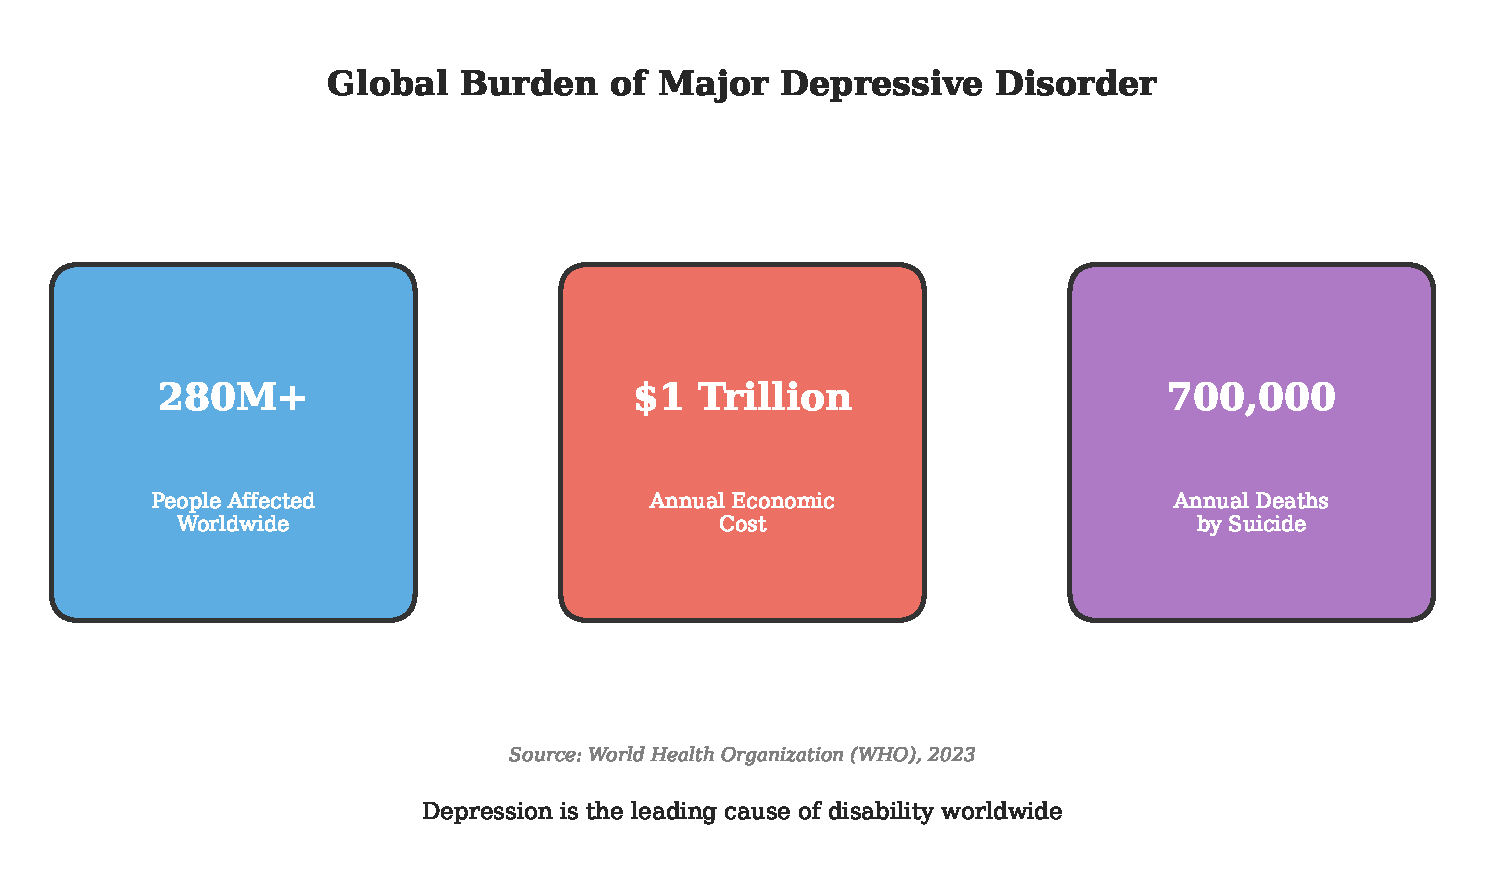
\includegraphics[width=0.85\textwidth]{figures/ch1/fig1_1_depression_statistics.pdf}
    \caption{Global burden of Major Depressive Disorder showing worldwide prevalence, economic impact, and mortality statistics.}
    \label{fig:depression_statistics}
\end{figure}

Despite this enormous burden, the diagnosis of depression remains fundamentally subjective. Clinicians rely primarily on structured interviews and self-reported symptom questionnaires such as the Patient Health Questionnaire-9 (PHQ-9) and Beck Depression Inventory-II (BDI-II). While these tools are clinically validated and widely used, they suffer from several inherent limitations that underscore the pressing need for objective biomarkers that can complement clinical judgment.

\subsection{Limitations of Current Diagnostic Approaches}

Current diagnostic methods for depression face significant challenges that limit their reliability and clinical utility. Inter-rater variability represents a fundamental problem, as different clinicians may arrive at different diagnoses for the same patient. This variability is particularly pronounced in mild-to-moderate cases where symptoms are less clearly defined, and the distinction between normal sadness and clinical depression requires subjective interpretation. Studies have shown that agreement between clinicians on depression diagnosis, even when using structured interviews, falls well short of perfect concordance.

Patient recall bias presents another significant limitation of questionnaire-based assessment. Self-reported instruments depend on patients accurately recalling and reporting their symptoms over the preceding one to two weeks, which is inherently unreliable. Depressed patients may exhibit cognitive symptoms including memory impairment and concentration difficulties that directly compromise their ability to accurately report their own mental state. Furthermore, the retrospective nature of these assessments means that current mood state can color recollection of past symptoms, leading to systematic biases in reporting.

Cultural and language barriers pose additional challenges to standardized assessment. Depression manifests differently across cultures, with some populations expressing psychological distress primarily through somatic symptoms rather than the cognitive and emotional symptoms emphasized in Western diagnostic frameworks. Standardized questionnaires developed and validated in one cultural context may not adequately capture the expression of depression in different populations, leading to systematic underdiagnosis in some groups.

The stigma surrounding mental illness contributes to underreporting of symptoms, as patients may minimize or deny their experiences due to concerns about social judgment, employment consequences, or internalized shame. This is particularly problematic in populations where mental health stigma remains high, and the resulting underreporting leads to delayed or missed diagnoses with corresponding delays in appropriate treatment.

Perhaps most fundamentally, current diagnostic approaches lack objective biomarkers. Unlike many medical conditions that can be confirmed through blood tests, imaging findings, or other physiological measurements, there is no laboratory test that definitively confirms depression. This absence of objective markers means that diagnosis relies entirely on patient report and clinical observation, with all the limitations these subjective assessments entail.

\subsection{EEG as a Potential Biomarker}

Electroencephalography offers a promising avenue for objective depression detection due to several advantageous characteristics that make it well-suited for clinical translation. EEG is entirely non-invasive, requiring only surface electrodes placed on the scalp to record the brain's electrical activity. Unlike invasive procedures or those requiring injection of contrast agents, EEG poses minimal risk to patients and can be repeated as often as clinically necessary without cumulative harm.

From an economic perspective, EEG equipment is significantly less expensive than alternative neuroimaging modalities such as MRI or PET scanners. A clinical-grade EEG system costs a fraction of what MRI installation and maintenance require, making EEG-based diagnostics potentially accessible to a much broader range of clinical settings, including primary care offices and community mental health centers where depression is most commonly encountered.

EEG provides exceptional temporal resolution, capturing neural activity at millisecond timescales that far exceed what is achievable with hemodynamic imaging methods like fMRI. This temporal precision is particularly valuable for depression research, as the neural dynamics associated with emotional processing and cognitive control operate on rapid timescales that EEG can resolve. The ability to track moment-to-moment fluctuations in brain activity provides rich information about the temporal dynamics of neural processing.

Most importantly for this project, decades of research have identified several EEG patterns that are consistently associated with depression and have been replicated across multiple independent studies. These established biomarkers provide a foundation for machine learning approaches and, crucially, offer a means to validate that learned models are capturing clinically meaningful patterns rather than spurious correlations.

\begin{figure}[H]
    \centering
    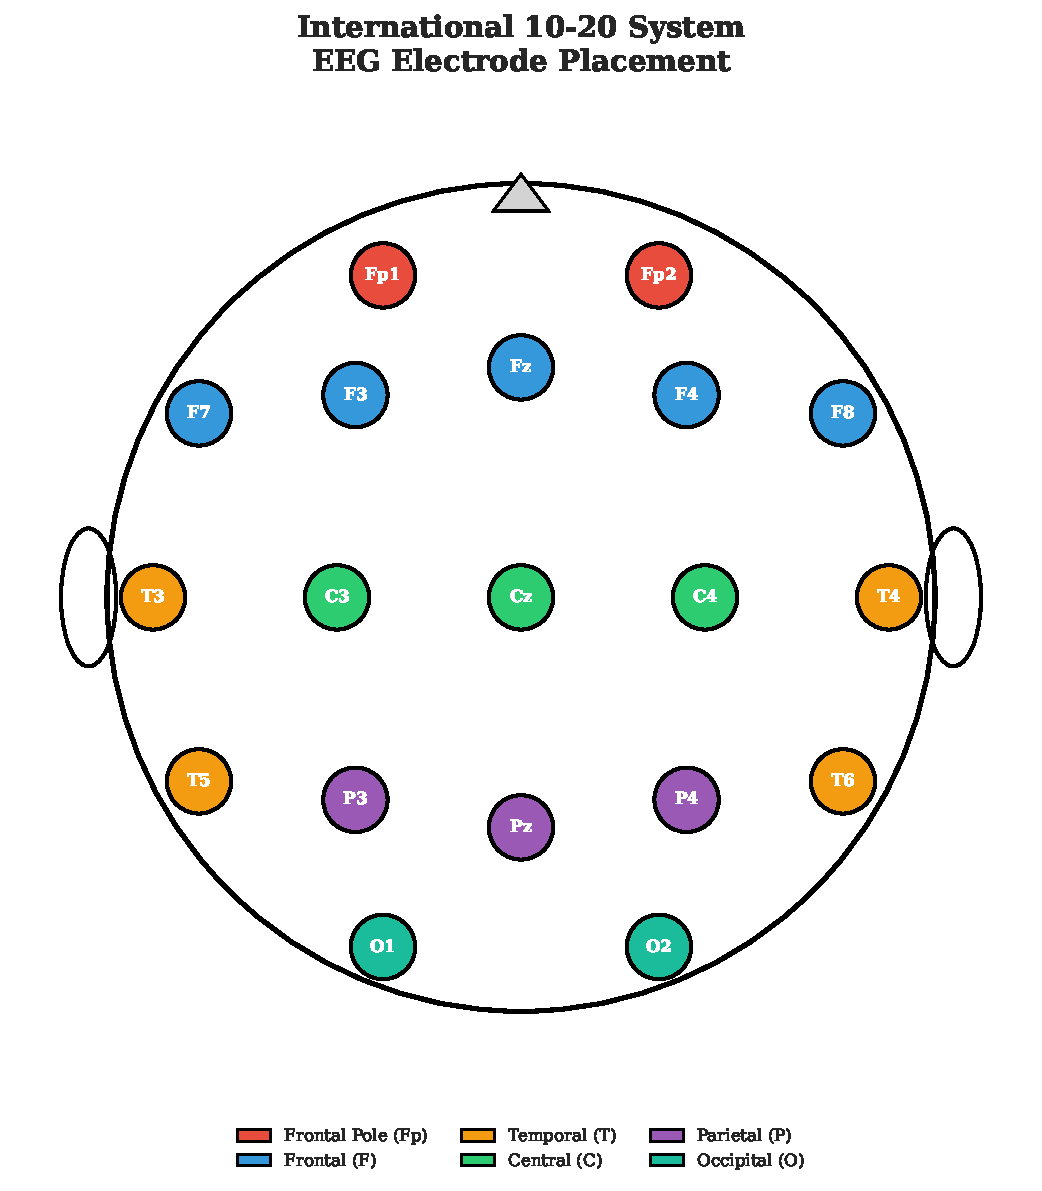
\includegraphics[width=0.75\textwidth]{figures/ch1/fig1_2_electrode_placement.pdf}
    \caption{International 10-20 System for EEG electrode placement showing the 19 standard electrode positions used in this study.}
    \label{fig:electrode_placement}
\end{figure}

Table \ref{tab:eeg_biomarkers} summarizes the established EEG biomarkers associated with depression that have been validated in clinical research. These biomarkers span multiple frequency bands and spatial locations, reflecting the distributed nature of the neural circuits involved in mood regulation.

\begin{table}[H]
    \centering
    \small
    \caption{EEG Biomarkers Associated with Major Depressive Disorder}
    \label{tab:eeg_biomarkers}
    \begin{tabularx}{\textwidth}{|L{2.8cm}|L{3.2cm}|X|L{2cm}|}
        \hline
        \textbf{Biomarker} & \textbf{Description} & \textbf{Clinical Significance} & \textbf{Reference} \\
        \hline
        Frontal Alpha Asymmetry (FAA) & Right $>$ Left frontal alpha power & Most validated depression biomarker; reflects approach/withdrawal motivation & \cite{henriques1991frontal} \\
        \hline
        Elevated Frontal Theta & Increased 4-8 Hz activity in frontal regions & Indicates frontal cortex dysfunction; predicts treatment response & \cite{arns2015frontal} \\
        \hline
        Alpha Power Reduction & Global decrease in 8-13 Hz activity & Common finding in depression; reflects reduced cortical arousal & \cite{knott2001eeg} \\
        \hline
        Delta Abnormality & Excessive slow-wave ($<$4 Hz) activity & Indicates cortical dysfunction in awake adults & \cite{davidson1998affective} \\
        \hline
        Reduced Coherence & Decreased inter-hemispheric connectivity & Reflects disrupted brain network integration & \cite{mumtaz2017machine} \\
        \hline
    \end{tabularx}
\end{table}

\subsection{The Data Leakage Problem in Existing Research}

A critical yet underappreciated issue plagues much of the published research on EEG-based depression detection: \textbf{data leakage} during cross-validation. Most studies employ standard k-fold cross-validation, which randomly splits samples into training and test sets without considering subject identity. This approach is fundamentally flawed for EEG analysis and leads to dramatically inflated performance estimates that do not reflect real-world generalization.

Consider a typical dataset where each subject contributes multiple EEG epochs, commonly ranging from 100 to 200 segments per subject depending on recording duration and epoch length. When standard k-fold cross-validation randomly assigns these samples to folds, epochs from the same subject inevitably appear in both training and test sets:

\begin{verbatim}
    INCORRECT: Standard 5-Fold Cross-Validation
    Subject A: [epoch1, epoch2, epoch3, ..., epoch100]
              randomly split
    Train set: [epoch1, epoch5, epoch8, ...]
    Test set:  [epoch2, epoch3, epoch9, ...]  <-- DATA LEAKAGE!
\end{verbatim}

In this scenario, the model can achieve artificially high accuracy by learning subject-specific patterns rather than depression-related patterns. Individual differences in skull thickness affect signal amplitude, electrode impedance varies across recordings, and each person's brain exhibits idiosyncratic activity patterns unrelated to psychopathology. When epochs from the same subject appear in both training and test sets, the model can exploit these subject-identifying characteristics to achieve seemingly impressive classification performance. This explains why many studies report accuracy values of 95-99\%---the models are essentially performing subject identification rather than disease detection.

The consequences of this methodological flaw become apparent when such models are deployed on truly new patients. Studies reporting 98\% accuracy with leaky validation would likely achieve only 60-75\% accuracy with proper subject-wise validation \cite{saeb2017need, varoquaux2017assessing}. This dramatic performance drop represents the gap between what the model actually learned (subject identity) and what it was supposed to learn (depression biomarkers).

\subsection{Our Solution: Honest Evaluation with LOSO}

This project addresses the data leakage problem by employing Leave-One-Subject-Out (LOSO) cross-validation, a rigorous evaluation protocol that ensures complete separation between training and test data at the subject level:

\begin{verbatim}
    CORRECT: LOSO Cross-Validation
    Fold 1: Train on Subjects [2, 3, 4, ..., 58]
            Test on Subject [1]  <-- NEVER SEEN BEFORE

    Fold 2: Train on Subjects [1, 3, 4, ..., 58]
            Test on Subject [2]  <-- NEVER SEEN BEFORE

    ... (58 folds total)
\end{verbatim}

In LOSO validation, each subject serves as the test set exactly once, while the model is trained on all remaining subjects. This ensures that the model must generalize to completely unseen individuals, precisely simulating the real clinical deployment scenario where a trained model encounters a new patient for the first time. No information about the test subject's brain activity patterns, recording characteristics, or individual idiosyncrasies can leak into training.

The expected accuracy with LOSO is necessarily lower than with leaky validation---typically 80-92\% versus 95-99\%. However, this lower number represents the \textit{true} performance that would be observed in actual clinical practice. A model achieving 91\% accuracy with LOSO validation is clinically far more valuable than one claiming 98\% accuracy with leaky validation, because the LOSO result honestly reflects how the system will perform when deployed. The apparent ``decrease'' in accuracy is actually an increase in honesty and clinical utility.

\section{CHAPTER-WISE SUMMARY}

This report is organized into five main chapters, each addressing a specific aspect of the EEG-based depression detection system.

\textbf{Chapter 1: Introduction} (Current Chapter) establishes the motivation for this work by discussing the global burden of depression, the limitations of current diagnostic approaches, and the potential of EEG as an objective biomarker. This chapter critically examines the data leakage problem that plagues existing research and introduces LOSO cross-validation as the methodologically sound solution that enables honest performance evaluation.

\textbf{Chapter 2: System Analysis} provides a detailed analysis of the existing system represented by the base paper from Khaleghi et al. (2025), systematically identifying its methodological limitations including data leakage, limited architecture capacity, and restricted explainability. The chapter then presents the proposed system with its key innovations, followed by use case analysis examining clinical screening, treatment monitoring, and research applications. The chapter concludes with comprehensive requirements specification including functional, non-functional, hardware, and software requirements.

\textbf{Chapter 3: System Design} describes the detailed system architecture including the complete processing pipeline from raw EEG signals to classification output. The methodology section covers data preprocessing with filtering and artifact removal, multi-wavelet feature extraction using both Wavelet Packet Decomposition and Continuous Wavelet Transform, the dual-branch Transformer-GNN model architecture, attention-based fusion mechanisms, and the LOSO training strategy. The chapter includes detailed module descriptions with input/output specifications and data design covering the Figshare MDD EEG dataset characteristics.

\textbf{Chapter 4: System Implementation} details the implementation of each module with relevant code excerpts and technical explanations. The testing and results section presents comprehensive evaluation including accuracy metrics, confusion matrix analysis, ROC curves, per-fold performance distribution, and direct comparison with the base paper. The chapter provides extensive explainability analysis results from Integrated Gradients and TCAV, demonstrating clinical validation of the learned biomarkers.

\textbf{Chapter 5: Conclusion and Future Scope} summarizes the key achievements and contributions of this work, including the 91.38\% subject-level accuracy achieved with honest LOSO validation and the clinical validation through explainability analysis. The chapter acknowledges current limitations including dataset size and single-site recording, then outlines future directions including the V2 model with Bi-LSTM, multi-site validation studies, depression severity prediction rather than binary classification, and potential pathways toward clinical deployment.

\textbf{Appendix A: Source Code} contains key excerpts from the implementation including the Transformer encoder, GNN encoder, attention fusion mechanism, and wavelet feature extraction modules, providing sufficient detail for reproducibility.

\textbf{Appendix B: Screenshots} provides visual documentation of the training process, results visualization, and explainability analysis outputs, illustrating the system's operation and results.



% Chapter 2: System Analysis
% ============================================================================
% CHAPTER 2: SYSTEM ANALYSIS
% ============================================================================

\chapter{SYSTEM ANALYSIS}

\section{EXISTING SYSTEM}

This section provides a detailed analysis of the base paper by Khaleghi et al. \cite{khaleghi2025interpretable}, published in MethodsX (2025), which serves as the primary reference point for understanding the current state of the art and identifying opportunities for improvement in EEG-based depression detection.

\subsection{Base Paper Overview}

The base paper presents an interpretable deep learning approach for depression detection using EEG signals, representing a recent contribution to the growing literature on automated psychiatric diagnosis. The authors utilize the Kaggle Depression-Rest EEG Dataset containing recordings from 232 patients and employ a relatively straightforward machine learning pipeline. Their approach begins with 31 pre-extracted features spanning six brain regions, applies Principal Component Analysis (PCA) for dimensionality reduction to 21 components, and feeds the resulting feature vectors into a two-layer convolutional neural network for classification. The paper incorporates SHAP (SHapley Additive exPlanations) for model interpretability and reports an impressive 98\% classification accuracy using 5-fold stratified cross-validation. Table \ref{tab:base_paper_summary} summarizes the key characteristics of this approach.

\begin{table}[H]
    \centering
    \small
    \caption{Summary of Base Paper Approach (Khaleghi et al., 2025)}
    \label{tab:base_paper_summary}
    \begin{tabularx}{\textwidth}{|L{3.5cm}|X|}
        \hline
        \textbf{Aspect} & \textbf{Description} \\
        \hline
        Dataset & Kaggle Depression-Rest EEG Dataset (232 patients) \\
        \hline
        Features & 31 pre-extracted features across 6 brain regions \\
        \hline
        Dimensionality Reduction & PCA (21 components) + t-SNE for visualization \\
        \hline
        Model Architecture & 2-layer CNN (64 and 128 filters) \\
        \hline
        Validation & 5-fold stratified cross-validation \\
        \hline
        Interpretability & SHAP (SHapley Additive exPlanations) \\
        \hline
        Reported Accuracy & 98\% \\
        \hline
    \end{tabularx}
\end{table}

\subsection{Base Paper Architecture}

The base paper employs a relatively simple convolutional neural network architecture consisting of two convolutional layers followed by fully connected layers for classification. The network receives the 21 PCA-reduced features as input, which are first reshaped into a single-channel one-dimensional signal format suitable for convolutional processing. The first convolutional layer applies 64 filters with kernel size 3, followed by max pooling that reduces the spatial dimension by half. The second convolutional layer increases the representational capacity with 128 filters, again followed by max pooling. After flattening the resulting feature maps, a dense layer with 64 units and ReLU activation provides the final feature transformation before the output layer produces class probabilities through softmax activation. Table \ref{tab:base_cnn_arch} details the complete architecture specifications, revealing a total parameter count of approximately 50,000---a relatively modest capacity for the complexity of the classification task.

\begin{table}[H]
    \centering
    \small
    \caption{Base Paper CNN Architecture Specifications}
    \label{tab:base_cnn_arch}
    \begin{tabularx}{\textwidth}{|l|l|l|X|}
        \hline
        \textbf{Layer} & \textbf{Type} & \textbf{Configuration} & \textbf{Output Shape} \\
        \hline
        Input & --- & 21 PCA features & (batch, 21) \\
        \hline
        Reshape & Reshape & --- & (batch, 1, 21) \\
        \hline
        Conv1 & Conv1D & 64 filters, kernel=3 & (batch, 64, 19) \\
        \hline
        Pool1 & MaxPool1D & pool\_size=2 & (batch, 64, 9) \\
        \hline
        Conv2 & Conv1D & 128 filters, kernel=3 & (batch, 128, 7) \\
        \hline
        Pool2 & MaxPool1D & pool\_size=2 & (batch, 128, 3) \\
        \hline
        Flatten & Flatten & --- & (batch, 384) \\
        \hline
        Dense1 & Dense & 64 units, ReLU & (batch, 64) \\
        \hline
        Output & Dense & 2 units, Softmax & (batch, 2) \\
        \hline
    \end{tabularx}
\end{table}

\begin{figure}[H]
    \centering
    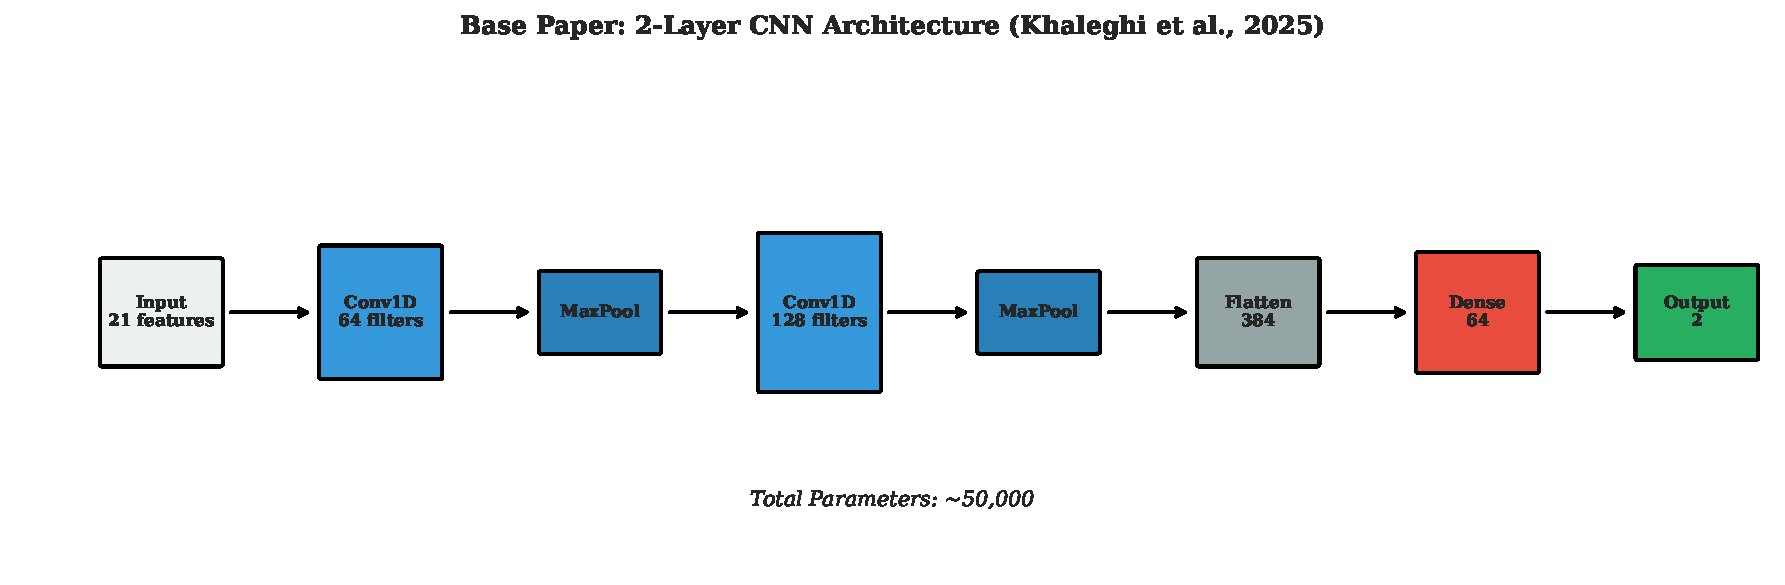
\includegraphics[width=0.9\textwidth]{figures/ch2/fig2_1_base_cnn.pdf}
    \caption{Base paper 2-layer CNN architecture for depression classification.}
    \label{fig:base_cnn_arch}
\end{figure}

\subsection{Base Paper Feature Extraction}

The base paper utilizes 31 pre-extracted features from the Kaggle dataset, organized into six categories spanning different aspects of EEG signal characterization. Spectral features capture band power in the standard frequency ranges including delta (1-4 Hz), theta (4-8 Hz), alpha (8-13 Hz), beta (13-30 Hz), and gamma (30-45 Hz) bands, computed using Fast Fourier Transform methods. Ratio features represent cross-band relationships such as delta-to-alpha and theta-to-beta power ratios, which have been associated with various cognitive and emotional states. Asymmetry features quantify hemispheric differences in power, particularly relevant given the established literature on frontal alpha asymmetry in depression. Entropy features based on wavelet decomposition provide measures of signal complexity and irregularity. Statistical features including mean, variance, and skewness capture basic distributional properties of the signals. Finally, regional features aggregate information across anatomically meaningful electrode groups including frontal, temporal, parietal, and occipital regions. Table \ref{tab:base_features} summarizes these feature categories.

\begin{table}[H]
    \centering
    \small
    \caption{Base Paper Feature Categories}
    \label{tab:base_features}
    \begin{tabularx}{\textwidth}{|L{2.5cm}|L{3.5cm}|X|}
        \hline
        \textbf{Category} & \textbf{Features} & \textbf{Description} \\
        \hline
        Spectral & Delta, Theta, Alpha, Beta, Gamma power & FFT-based band power in standard frequency bands \\
        \hline
        Ratio Features & Delta/Alpha, Theta/Beta ratios & Cross-band power ratios \\
        \hline
        Asymmetry & Left-Right differences & Hemispheric power differences \\
        \hline
        Entropy & Wavelet entropy & Signal complexity measure \\
        \hline
        Statistical & Mean, variance, skewness & Basic statistical moments \\
        \hline
        Regional & Frontal, temporal, parietal, occipital & Region-specific aggregations \\
        \hline
    \end{tabularx}
\end{table}

\begin{figure}[H]
    \centering
    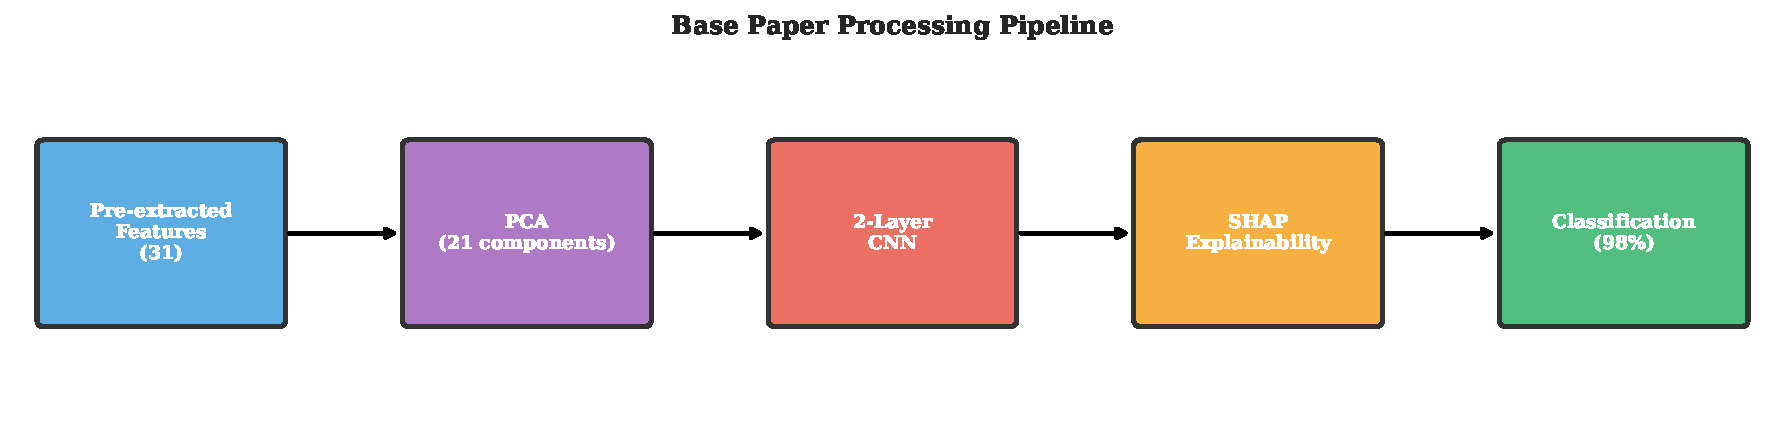
\includegraphics[width=0.9\textwidth]{figures/ch2/fig2_2_base_pipeline.pdf}
    \caption{Base paper processing pipeline showing the flow from pre-extracted features to classification.}
    \label{fig:base_pipeline}
\end{figure}

\subsection{Critical Analysis of Base Paper Limitations}

While the base paper reports impressive results, our thorough analysis reveals several significant methodological limitations that fundamentally undermine the clinical utility and scientific validity of the reported findings.

\subsubsection{Limitation 1: Data Leakage in Cross-Validation}

The most critical limitation is the use of standard 5-fold cross-validation without subject-wise splitting, which introduces severe data leakage that invalidates the reported performance metrics. With 232 patients contributing multiple samples each, random splitting inevitably causes epochs from the same subject to appear in both training and test sets. This allows the model to achieve artificially high accuracy by learning subject-specific patterns rather than depression-related patterns.

Several pieces of evidence strongly suggest the presence of data leakage in the reported results. The claimed 98\% accuracy is suspiciously high for a complex psychiatric classification task, as even expert clinicians do not achieve such reliability in depression diagnosis. Furthermore, the model confidence scores reported in the paper range from 0.41 to 0.59 despite the 98\% accuracy, revealing poor calibration that would not be expected from a model genuinely learning disease-relevant patterns. Most tellingly, the paper reports only sample-level accuracy metrics without any subject-level evaluation, obscuring whether the model generalizes to new individuals or merely memorizes subject-specific characteristics.

\subsubsection{Limitation 2: Pre-Extracted Features}

The reliance on pre-extracted features from the Kaggle dataset severely limits methodological control and constrains the potential for innovation. Working with pre-extracted features means researchers cannot apply custom wavelet families that might be optimized for depression-specific frequency patterns. The fixed feature set prevents generation of time-frequency representations such as scalograms that would enable more sophisticated deep learning architectures like Transformers. Experimentation with different preprocessing pipelines---including alternative filtering parameters, artifact rejection strategies, or epoch segmentation approaches---becomes impossible when starting from pre-extracted features. Additionally, the aggregated regional features preclude extraction of channel-wise information necessary for graph-based spatial modeling that could capture electrode relationships. These constraints fundamentally limit the scientific exploration possible within this framework.

\subsubsection{Limitation 3: Simple Architecture}

The 2-layer CNN architecture, while computationally efficient, has severely limited representational capacity that constrains its ability to learn the complex patterns associated with depression. Convolutional layers with small kernels can only capture local patterns and cannot model long-range temporal dependencies that are crucial for EEG rhythms spanning multiple cycles. The architecture includes no mechanism for explicitly modeling spatial relationships between electrodes, treating the input as a simple one-dimensional sequence rather than a spatially organized array of sensors. The limited receptive field prevents the network from recognizing complex patterns that span the full input, and the approximately 50,000 parameters provide insufficient capacity for learning the nuanced feature transformations needed to distinguish depression from healthy brain states.

\subsubsection{Limitation 4: Limited Explainability}

While the base paper incorporates SHAP for model interpretability, this provides only a single, limited view of model decision-making that falls short of clinical requirements for understanding automated diagnostic systems. SHAP analysis reveals which input features contribute to predictions but cannot validate whether the model has learned specific clinical concepts that clinicians recognize and trust. There is no layer-wise understanding of how information flows through the network, making it difficult to understand what transformations the model applies to raw features. Most critically, SHAP cannot directly test hypotheses about whether the model uses established depression biomarkers such as frontal alpha asymmetry or elevated theta power, leaving uncertainty about the clinical validity of the learned representations.

\begin{figure}[H]
    \centering
    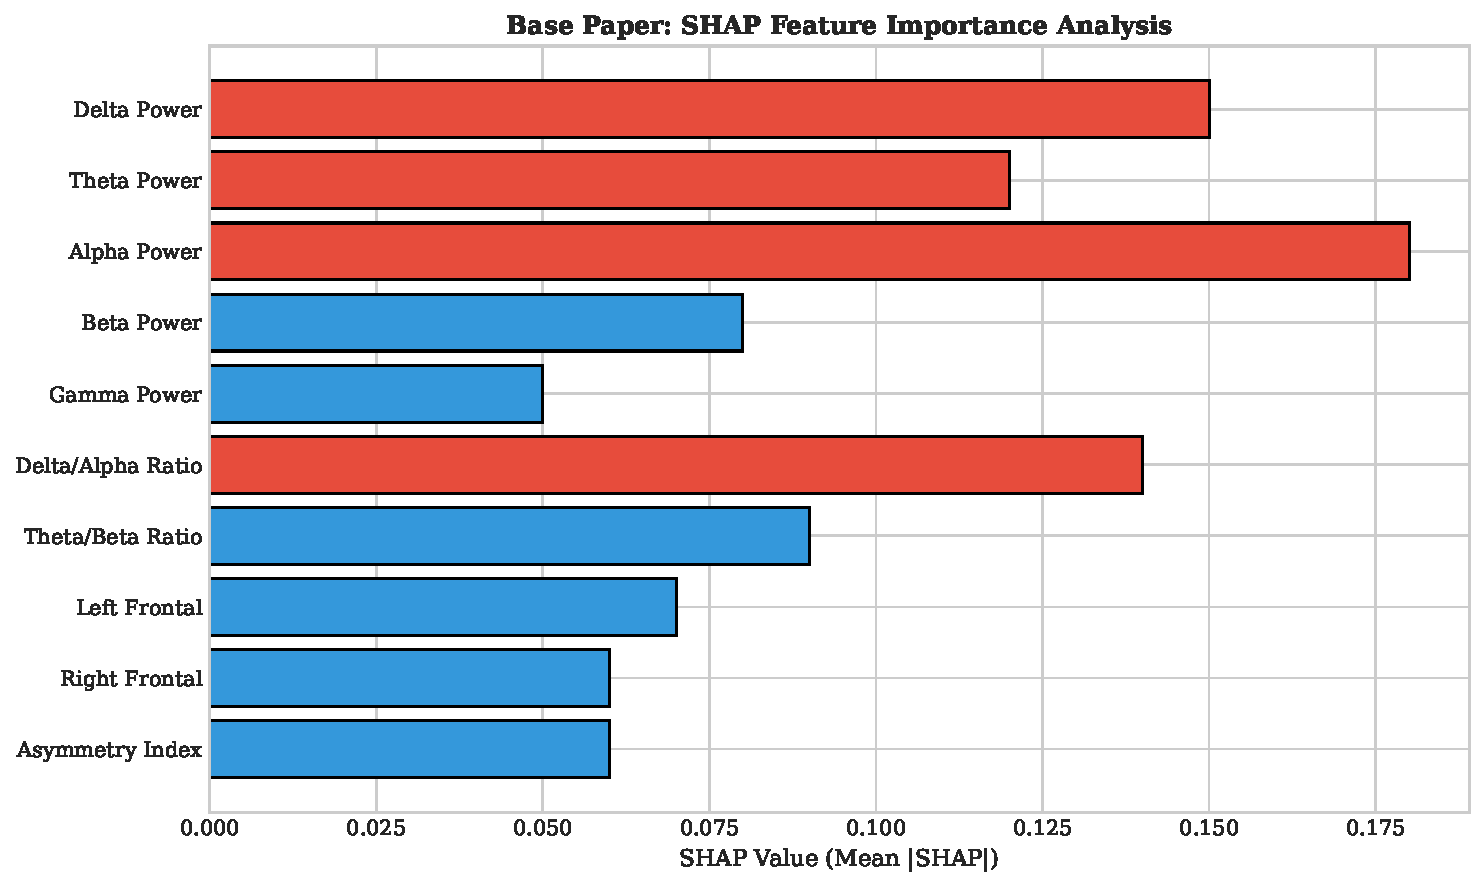
\includegraphics[width=0.85\textwidth]{figures/ch2/fig2_3_shap_importance.pdf}
    \caption{Base paper SHAP feature importance analysis showing contribution of different features to model predictions.}
    \label{fig:base_shap}
\end{figure}

\subsection{Expected Real-World Performance}

Based on our analysis and the established literature on evaluation methodology in biomedical machine learning \cite{saeb2017need, varoquaux2017assessing}, we can estimate the base paper's expected real-world performance when deployed on truly new patients. The gap between reported performance and expected clinical performance is stark. While the paper claims 98\% accuracy, proper subject-wise validation would likely yield only 60-70\% accuracy---barely above chance for some samples. The claimed high clinical utility would evaporate, as a model that cannot generalize to new individuals provides no diagnostic value. What the model actually learns under leaky validation is subject identity rather than depression patterns, making it fundamentally unsuitable for clinical deployment where each patient is new. Table \ref{tab:base_real_performance} summarizes this discrepancy between reported and expected performance.

\begin{table}[H]
    \centering
    \small
    \caption{Base Paper Results: Reported vs. Expected Real-World Performance}
    \label{tab:base_real_performance}
    \begin{tabularx}{\textwidth}{|X|c|c|}
        \hline
        \textbf{Metric} & \textbf{Reported (Leaky CV)} & \textbf{Expected (LOSO)} \\
        \hline
        Accuracy & 98\% & 60-70\% \\
        \hline
        Clinical Utility & Claimed high & None (cannot generalize) \\
        \hline
        What Model Learns & Depression patterns & Subject identity \\
        \hline
        Deployment Feasibility & Yes (per paper) & No (would fail) \\
        \hline
    \end{tabularx}
\end{table}

\section{PROPOSED SYSTEM}

Our proposed system addresses all identified limitations through fundamental methodological improvements and advanced architecture design, creating a framework that can deliver honest performance metrics and clinically validated predictions.

\subsection{Key Innovations}

The proposed system introduces comprehensive improvements across every aspect of the EEG-based depression detection pipeline. Table \ref{tab:detailed_comparison} presents a detailed comparison between the base paper approach and our proposed system, highlighting the fundamental differences in methodology, architecture, and evaluation.

\begin{table}[H]
    \centering
    \small
    \caption{Detailed Comparison: Base Paper vs. Proposed System}
    \label{tab:detailed_comparison}
    \begin{tabularx}{\textwidth}{|L{3cm}|L{4.5cm}|X|}
        \hline
        \textbf{Aspect} & \textbf{Base Paper} & \textbf{Proposed System} \\
        \hline
        Dataset Type & Pre-extracted features & Raw EEG signals \\
        \hline
        Feature Extraction & 31 fixed features & 576 features/channel (WPD) + CWT scalograms \\
        \hline
        Wavelet Analysis & Single wavelet (unspecified) & Multi-wavelet: db4, sym5, coif3 \\
        \hline
        Time-Frequency & Not used & CWT scalograms (64$\times$128) \\
        \hline
        Architecture & 2-layer CNN & Transformer + GNN fusion \\
        \hline
        Spatial Modeling & None (flat feature vector) & Graph Attention Network \\
        \hline
        Temporal Modeling & Conv1D (local) & Transformer (global attention) \\
        \hline
        Parameters & $\sim$50K & $\sim$1.55M \\
        \hline
        Cross-Validation & 5-fold (leaky) & LOSO (no leakage) \\
        \hline
        Explainability & SHAP only & IG + LRP + TCAV \\
        \hline
        Reported Accuracy & 98\% (inflated) & 91.38\% (honest) \\
        \hline
        Clinical Validity & Questionable & Validated biomarkers \\
        \hline
    \end{tabularx}
\end{table}

\subsection{Proposed Architecture Overview}

The proposed system employs a sophisticated dual-branch architecture that captures complementary information from EEG signals, combining the strengths of modern deep learning approaches for both temporal and spatial analysis.

The Transformer Branch processes Continuous Wavelet Transform scalograms using a Vision Transformer architecture adapted for time-frequency analysis. The scalogram representation encodes how spectral content evolves over the 4-second epoch, providing a rich two-dimensional input that captures both the frequency composition and its temporal dynamics. The Transformer's self-attention mechanism enables the model to identify which frequency components at which time points are most relevant for depression detection, learning global dependencies that span the entire time-frequency representation. This addresses the limited receptive field problem of convolutional approaches by allowing every position to attend to every other position.

The GNN Branch processes Wavelet Packet Decomposition features using a Graph Attention Network that explicitly models the spatial relationships between EEG electrodes. Rather than treating electrodes as independent or as a simple sequence, the GNN represents them as nodes in a graph where edges encode both physical proximity based on the 10-20 electrode montage and functional connectivity estimated from signal correlations. The graph attention mechanism learns which electrode connections are most informative for depression detection, capturing the distributed brain network dynamics that characterize mood disorders. This spatial modeling capability is entirely absent from the base paper approach.

The Attention-Based Fusion module combines features from both branches using a learned cross-attention mechanism that adaptively weights their contributions. The Transformer branch captures time-frequency patterns while the GNN branch captures spatial patterns, and fusion learns how to optimally combine these complementary views based on the characteristics of each input. This adaptive combination is superior to simple concatenation or averaging, as it allows the model to emphasize whichever modality is more informative for each particular sample.

The Classification Head receives the fused representation and produces the final binary classification through a multi-layer perceptron with batch normalization and dropout for regularization. The output is a probability score between 0 and 1 indicating the likelihood of Major Depressive Disorder, which can be thresholded for binary classification or used directly for probabilistic reasoning about diagnostic confidence.

\begin{figure}[H]
    \centering
    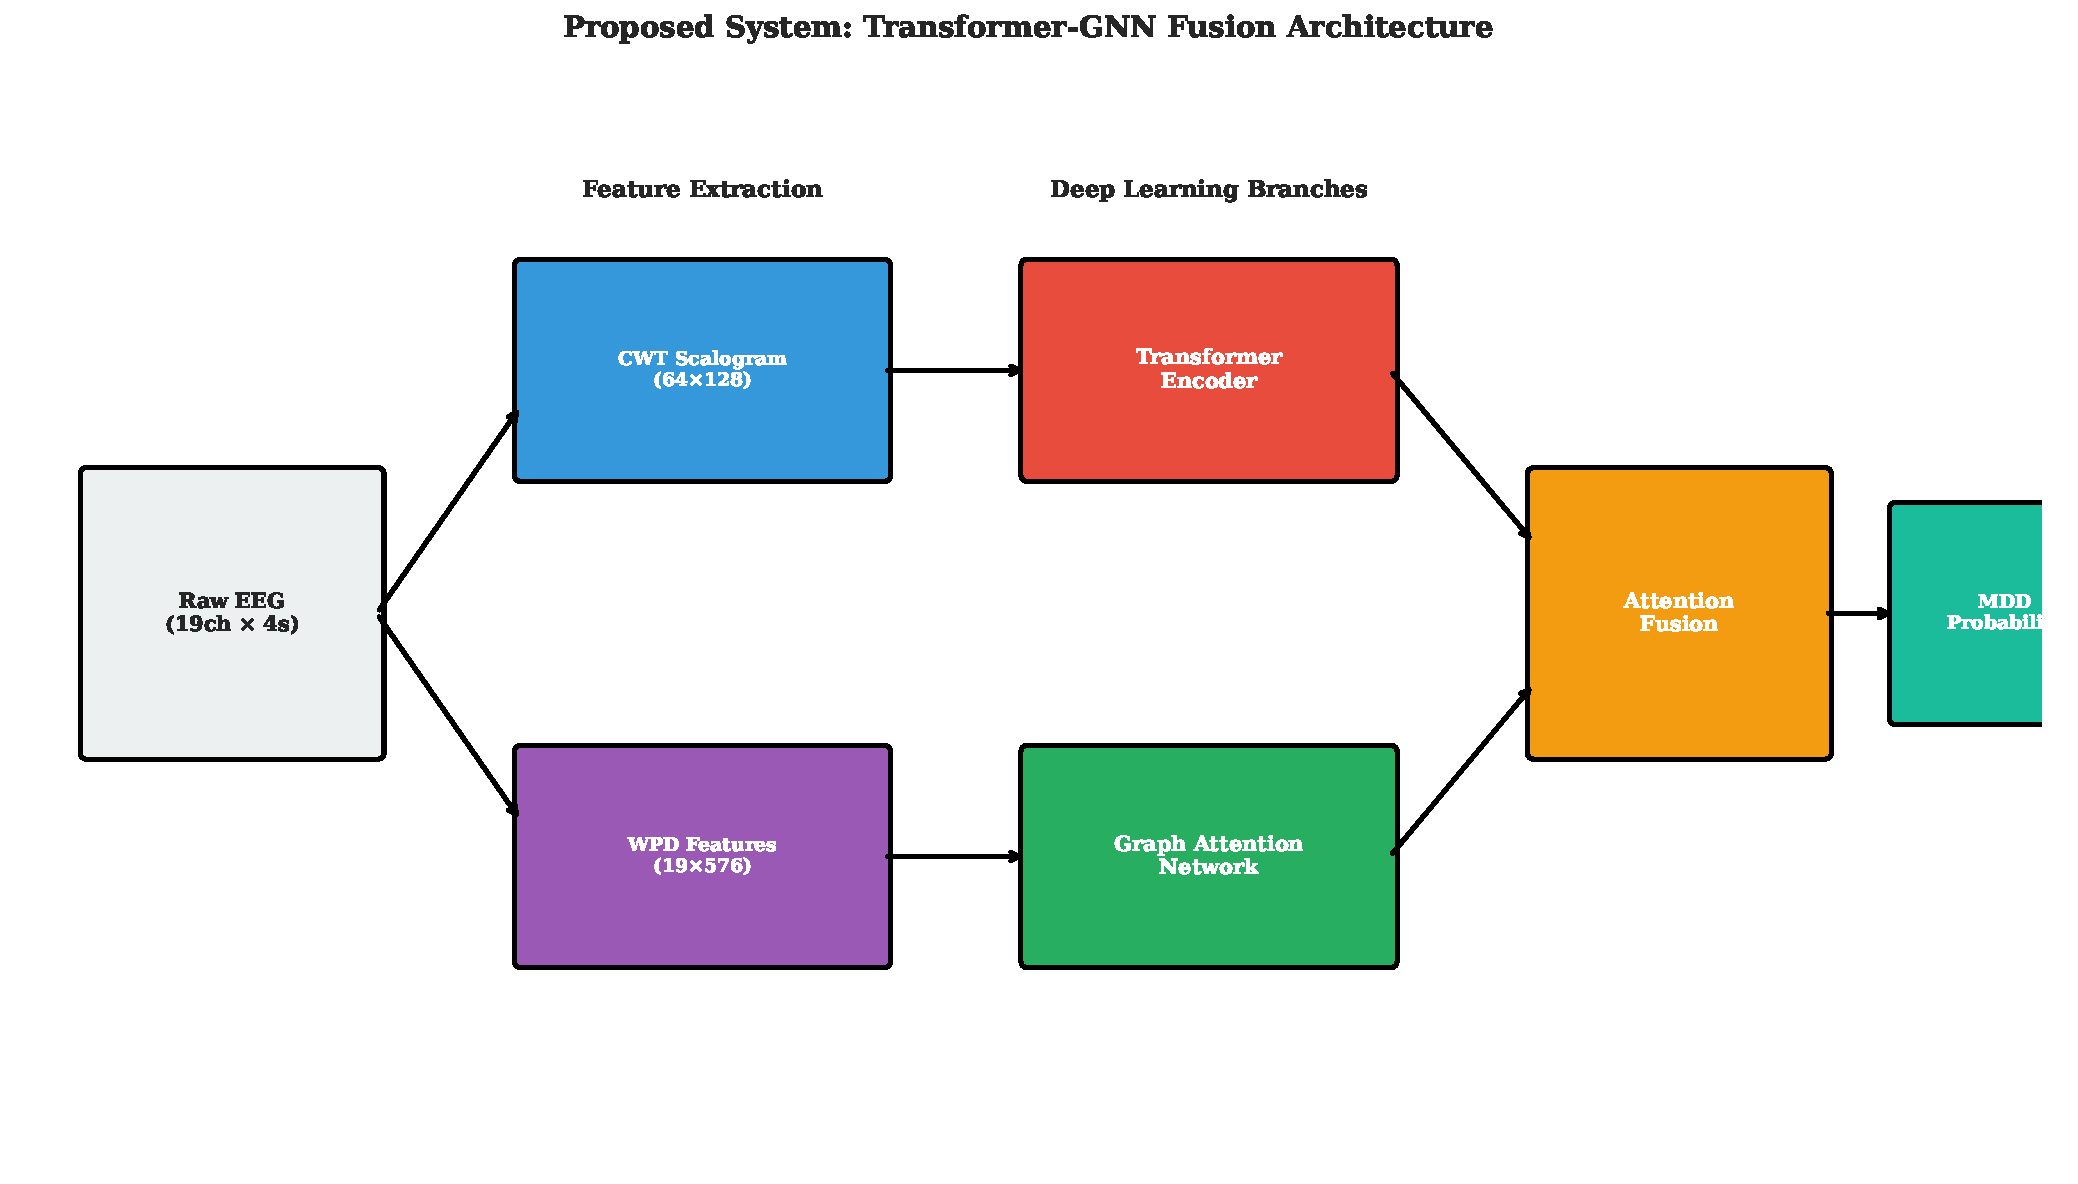
\includegraphics[width=0.95\textwidth]{figures/ch2/fig2_4_proposed_architecture.pdf}
    \caption{Proposed dual-branch architecture combining Transformer for time-frequency analysis and GNN for spatial modeling, with attention-based fusion.}
    \label{fig:proposed_arch}
\end{figure}

\begin{figure}[H]
    \centering
    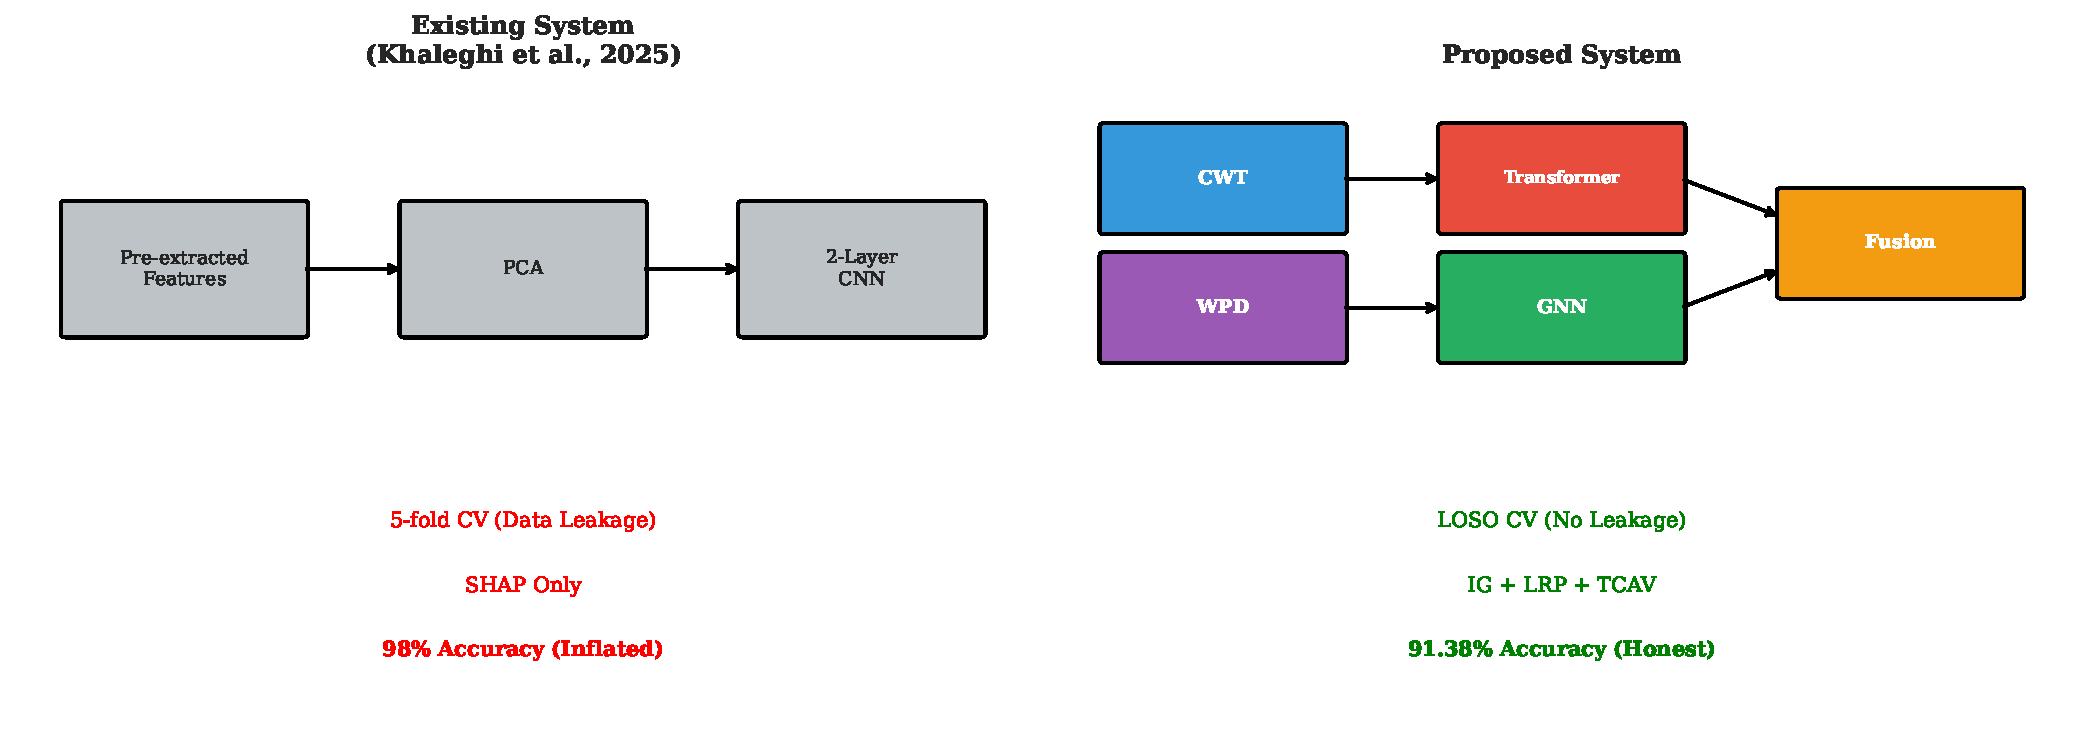
\includegraphics[width=0.95\textwidth]{figures/ch2/fig2_5_comparison.pdf}
    \caption{Visual comparison of existing system (base paper) and proposed system architectures.}
    \label{fig:system_comparison}
\end{figure}

\subsection{Summary of Key Innovations}

The innovations introduced by the proposed system span methodology, architecture, and evaluation, each addressing specific limitations of the existing approach. Table \ref{tab:innovations} summarizes these innovations with their functional descriptions and significance for clinical depression detection.

\begin{table}[H]
    \centering
    \small
    \caption{Summary of Key Innovations in Proposed System}
    \label{tab:innovations}
    \begin{tabularx}{\textwidth}{|L{2.8cm}|L{3.8cm}|X|}
        \hline
        \textbf{Innovation} & \textbf{What It Does} & \textbf{Why It Matters} \\
        \hline
        Raw Signal Processing & Extract features from original EEG & Full control over feature engineering \\
        \hline
        Multi-Wavelet WPD & Use db4, sym5, coif3 wavelets & Captures diverse spectral characteristics \\
        \hline
        CWT Scalograms & Time-frequency 2D representation & Enables Transformer-based processing \\
        \hline
        Transformer Encoder & Global self-attention on scalograms & Captures long-range dependencies \\
        \hline
        Graph Attention Network & Models electrode relationships & Captures spatial brain connectivity \\
        \hline
        Attention Fusion & Adaptive branch combination & Leverages complementary information \\
        \hline
        LOSO Validation & Subject-wise test splits & Prevents data leakage, honest evaluation \\
        \hline
        Multi-Level XAI & IG + LRP + TCAV & Validates clinical biomarker learning \\
        \hline
    \end{tabularx}
\end{table}

\section{USE CASE ANALYSIS}

This section presents the primary use cases for the EEG-based depression detection system, examining how different stakeholders would interact with the system in realistic deployment scenarios.

\begin{figure}[H]
    \centering
    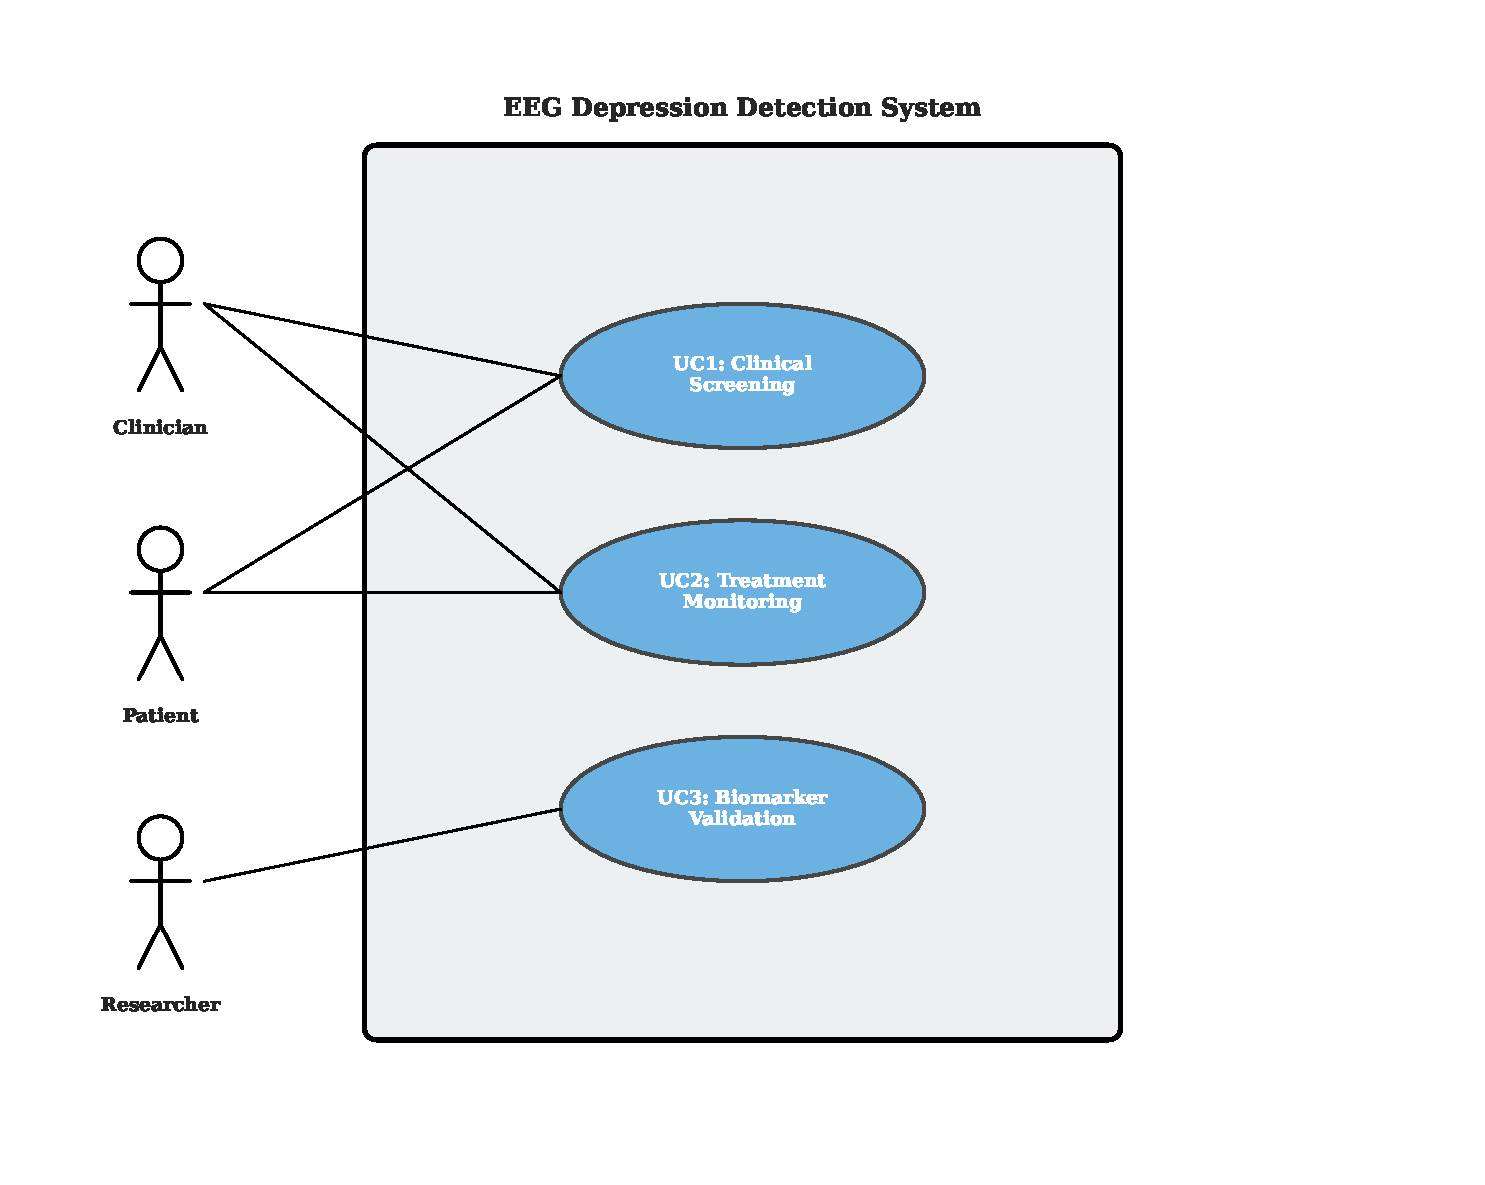
\includegraphics[width=0.85\textwidth]{figures/ch2/fig2_6_use_case.pdf}
    \caption{Use case diagram showing primary actors and use cases for the EEG-based depression detection system.}
    \label{fig:use_case}
\end{figure}

\subsection{Use Case 1: Clinical Screening for Depression}

The primary clinical use case involves a psychiatrist or general practitioner seeking objective supplementary information to support depression diagnosis. The scenario begins when a patient presents with symptoms suggestive of depression, such as persistent low mood, loss of interest, sleep disturbances, or cognitive difficulties. The clinician, having access to EEG recording equipment and the deployed trained model, decides to obtain objective biomarker data to complement the clinical interview and standardized questionnaires.

The patient undergoes a brief 5-minute eyes-closed resting state EEG recording using the standard 19-electrode 10-20 montage. This recording protocol requires minimal patient cooperation and can be conducted in a standard clinical environment. Once the recording is complete, the system automatically preprocesses the raw EEG signals, applying bandpass and notch filtering, artifact rejection, and epoch segmentation. The feature extraction modules compute both WPD features for the GNN branch and CWT scalograms for the Transformer branch.

The trained model then generates a depression probability score along with a confidence estimate, providing the clinician with a quantitative assessment of the likelihood that the patient's brain activity patterns are consistent with Major Depressive Disorder. Critically, the explainability analysis module provides biomarker-level interpretation, showing which electrodes and frequency bands contributed most to the prediction and whether the model's reasoning aligns with established depression biomarkers such as frontal alpha asymmetry.

The clinician reviews these objective results alongside their clinical assessment, using the model output as one piece of evidence among many in formulating a diagnosis. The results are documented in the patient's electronic health record for future reference, and the objective trajectory of biomarker changes can inform treatment planning and monitoring decisions.

\subsection{Use Case 2: Treatment Response Monitoring}

The second major use case addresses the challenge of tracking treatment response objectively over time. Depression treatment, whether pharmacological or psychotherapeutic, often requires weeks to months to produce clinically meaningful improvement, and subjective symptom reports may not accurately reflect underlying neurophysiological changes. EEG biomarkers offer the potential to detect treatment response earlier and more objectively than self-report measures alone.

In this scenario, a baseline EEG is recorded at treatment initiation, establishing the patient's pre-treatment biomarker profile. The system stores the model's predictions and the detailed explainability analysis, including electrode importance maps and TCAV concept scores. As treatment progresses, follow-up EEG recordings are obtained at regular intervals---for example, at 2, 4, and 8 weeks after treatment initiation.

The system compares depression probability scores across these time points, generating a trajectory plot showing how the objective biomarker assessment evolves during treatment. Changes in the underlying biomarker patterns are visualized through comparative explainability analysis, allowing clinicians to observe whether frontal alpha asymmetry is normalizing, whether elevated theta power is decreasing, or whether other neurophysiological changes consistent with treatment response are emerging.

This objective trajectory data informs treatment decisions, providing evidence to support continuing an effective treatment, adjusting dosage, switching medications, or augmenting with additional interventions. The ability to detect neurophysiological changes before subjective symptom improvement becomes apparent could accelerate treatment optimization and reduce the duration of inadequately treated depression.

\subsection{Use Case 3: Research Biomarker Validation}

The third use case addresses the needs of clinical researchers seeking to validate novel EEG biomarkers for depression using the system's explainability capabilities. Unlike clinical deployment where the model serves as a diagnostic aid, research applications focus on using the trained model as a tool for hypothesis testing and biomarker discovery.

A researcher interested in a specific clinical concept---such as ``elevated theta power in frontal regions'' or ``reduced interhemispheric coherence''---can use the TCAV analysis to test whether the trained model has learned to use this concept in its classification decisions. By providing positive and negative examples of the concept, TCAV computes a score indicating how strongly the model relies on that concept when predicting depression.

Complementary Integrated Gradients and LRP analyses reveal which specific input features correspond to the high-level concept, providing fine-grained attribution that links abstract clinical concepts to concrete signal characteristics. Statistical analysis across the dataset validates whether the identified patterns correlate with depression at the population level, distinguishing genuine biomarkers from spurious correlations that might arise in individual subjects.

The results of such analyses contribute to the clinical knowledge base, potentially identifying novel biomarkers, refining understanding of established biomarkers, or revealing interactions between multiple biomarkers that have not been previously characterized. This research use case leverages the interpretability of the proposed system to advance scientific understanding beyond mere classification accuracy.

\section{REQUIREMENTS SPECIFICATION}

\subsection{Functional Requirements}

The functional requirements specify what the system must do to fulfill its intended purpose. Table \ref{tab:functional_req} presents the complete functional requirements specification, covering the full pipeline from data loading through result reporting.

\begin{table}[H]
    \centering
    \small
    \caption{Functional Requirements Specification}
    \label{tab:functional_req}
    \begin{tabularx}{\textwidth}{|L{1.2cm}|L{3.5cm}|X|}
        \hline
        \textbf{ID} & \textbf{Requirement} & \textbf{Description} \\
        \hline
        FR1 & Load Raw EEG Data & System shall load EEG data in EDF format from the Figshare dataset \\
        \hline
        FR2 & Preprocess EEG Signals & System shall apply bandpass filtering (1-45 Hz), notch filtering (50/60 Hz), and artifact rejection \\
        \hline
        FR3 & Extract WPD Features & System shall compute Wavelet Packet Decomposition features using db4, sym5, and coif3 wavelets \\
        \hline
        FR4 & Generate CWT Scalograms & System shall generate 64$\times$128 CWT scalograms using Complex Morlet wavelet \\
        \hline
        FR5 & Train Deep Learning Model & System shall train the Transformer-GNN fusion model using LOSO cross-validation \\
        \hline
        FR6 & Generate Predictions & System shall output depression probability (0-1) for each input epoch \\
        \hline
        FR7 & Compute Explainability & System shall provide Integrated Gradients, LRP, and TCAV explanations \\
        \hline
        FR8 & Report Results & System shall generate comprehensive metrics including accuracy, AUC-ROC, F1-score, confusion matrix \\
        \hline
    \end{tabularx}
\end{table}

\subsection{Non-Functional Requirements}

The non-functional requirements specify quality attributes and constraints on how the system performs its functions. Table \ref{tab:nonfunctional_req} presents requirements spanning performance, memory efficiency, accuracy targets, and software quality attributes.

\begin{table}[H]
    \centering
    \small
    \caption{Non-Functional Requirements Specification}
    \label{tab:nonfunctional_req}
    \begin{tabularx}{\textwidth}{|L{2.5cm}|L{3.5cm}|X|}
        \hline
        \textbf{Category} & \textbf{Requirement} & \textbf{Specification} \\
        \hline
        Performance & Inference Time & Process one 4-second epoch in $<$ 1 second \\
        \hline
        Performance & Training Time & Complete LOSO (58 folds) in $<$ 15 hours \\
        \hline
        Memory & GPU VRAM & Run on GPU with $\leq$ 8 GB VRAM \\
        \hline
        Memory & System RAM & Require $\leq$ 16 GB system RAM \\
        \hline
        Accuracy & Subject Accuracy & Achieve $>$ 85\% subject-level accuracy on LOSO \\
        \hline
        Accuracy & AUC-ROC & Achieve $>$ 0.85 area under ROC curve \\
        \hline
        Reliability & Reproducibility & Results reproducible with fixed random seeds \\
        \hline
        Maintainability & Modularity & Code organized in modular, documented components \\
        \hline
    \end{tabularx}
\end{table}

\subsection{Hardware and Software Requirements}

The system is designed to run on accessible hardware configurations commonly available in academic and clinical research settings. Table \ref{tab:hw_sw_req} specifies the minimum hardware requirements and software dependencies necessary for system deployment.

\begin{table}[H]
    \centering
    \small
    \caption{Hardware and Software Requirements}
    \label{tab:hw_sw_req}
    \begin{tabularx}{\textwidth}{|L{2.5cm}|L{3.5cm}|X|}
        \hline
        \textbf{Category} & \textbf{Requirement} & \textbf{Specification} \\
        \hline
        \multicolumn{3}{|l|}{\textbf{Hardware Requirements}} \\
        \hline
        GPU & NVIDIA GPU & RTX 4070 or equivalent (8 GB VRAM minimum) \\
        \hline
        RAM & System Memory & 16 GB minimum, 32 GB recommended \\
        \hline
        Storage & Disk Space & 5 GB for dataset, code, and outputs \\
        \hline
        CPU & Processor & Multi-core processor (Intel/AMD) \\
        \hline
        \multicolumn{3}{|l|}{\textbf{Software Requirements}} \\
        \hline
        OS & Operating System & Ubuntu 20.04+ / Windows 10+ \\
        \hline
        Language & Python & Version 3.10 or higher \\
        \hline
        Deep Learning & PyTorch & Version 2.0 or higher \\
        \hline
        Graph ML & PyTorch Geometric & Version 2.3 or higher \\
        \hline
        Signal Processing & MNE-Python & Version 1.5 or higher \\
        \hline
        Wavelets & PyWavelets & Version 1.4 or higher \\
        \hline
        Explainability & Captum & Version 0.6 or higher \\
        \hline
        Scientific & NumPy, SciPy, scikit-learn & Latest stable versions \\
        \hline
    \end{tabularx}
\end{table}



% Chapter 3: System Design
% ============================================================================
% CHAPTER 3: SYSTEM DESIGN
% ============================================================================

\chapter{SYSTEM DESIGN}

\section{SYSTEM ARCHITECTURE}

This section presents the detailed architecture of the EEG-based depression detection system, describing the complete processing pipeline from raw signal acquisition through classification and explainability analysis. The architecture reflects a careful balance between model expressiveness, computational efficiency, and interpretability requirements.

\subsection{Complete Pipeline Overview}

The system processes raw EEG signals through a multi-stage pipeline that transforms continuous recordings into depression classification predictions accompanied by comprehensive explainability outputs. The pipeline begins with data loading, where EDF-format recordings are parsed to extract the 19-channel EEG signals. These raw signals undergo extensive preprocessing including filtering, artifact removal, and epoch segmentation to produce clean, standardized input suitable for feature extraction.

The feature extraction stage branches into two parallel pathways. The first pathway computes Wavelet Packet Decomposition features that capture fine-grained spectral information across 32 frequency subbands, yielding 576 features per channel that serve as node attributes for the Graph Attention Network. The second pathway generates Continuous Wavelet Transform scalograms that represent the time-frequency evolution of the signal in a 64×128 image format suitable for the Vision Transformer. These parallel feature representations feed into their respective model branches, which process the information through specialized architectures optimized for their input modalities.

The Transformer and GNN branches produce fixed-dimensional feature vectors that are combined through an attention-based fusion module. This fusion mechanism learns to adaptively weight the contributions from each branch based on the characteristics of the input, producing a unified representation that captures both time-frequency patterns and spatial electrode relationships. The fused features pass through a classification head that outputs a depression probability, and the complete forward pass supports gradient-based explainability methods that reveal which input features drove the prediction.

\begin{figure}[H]
    \centering
    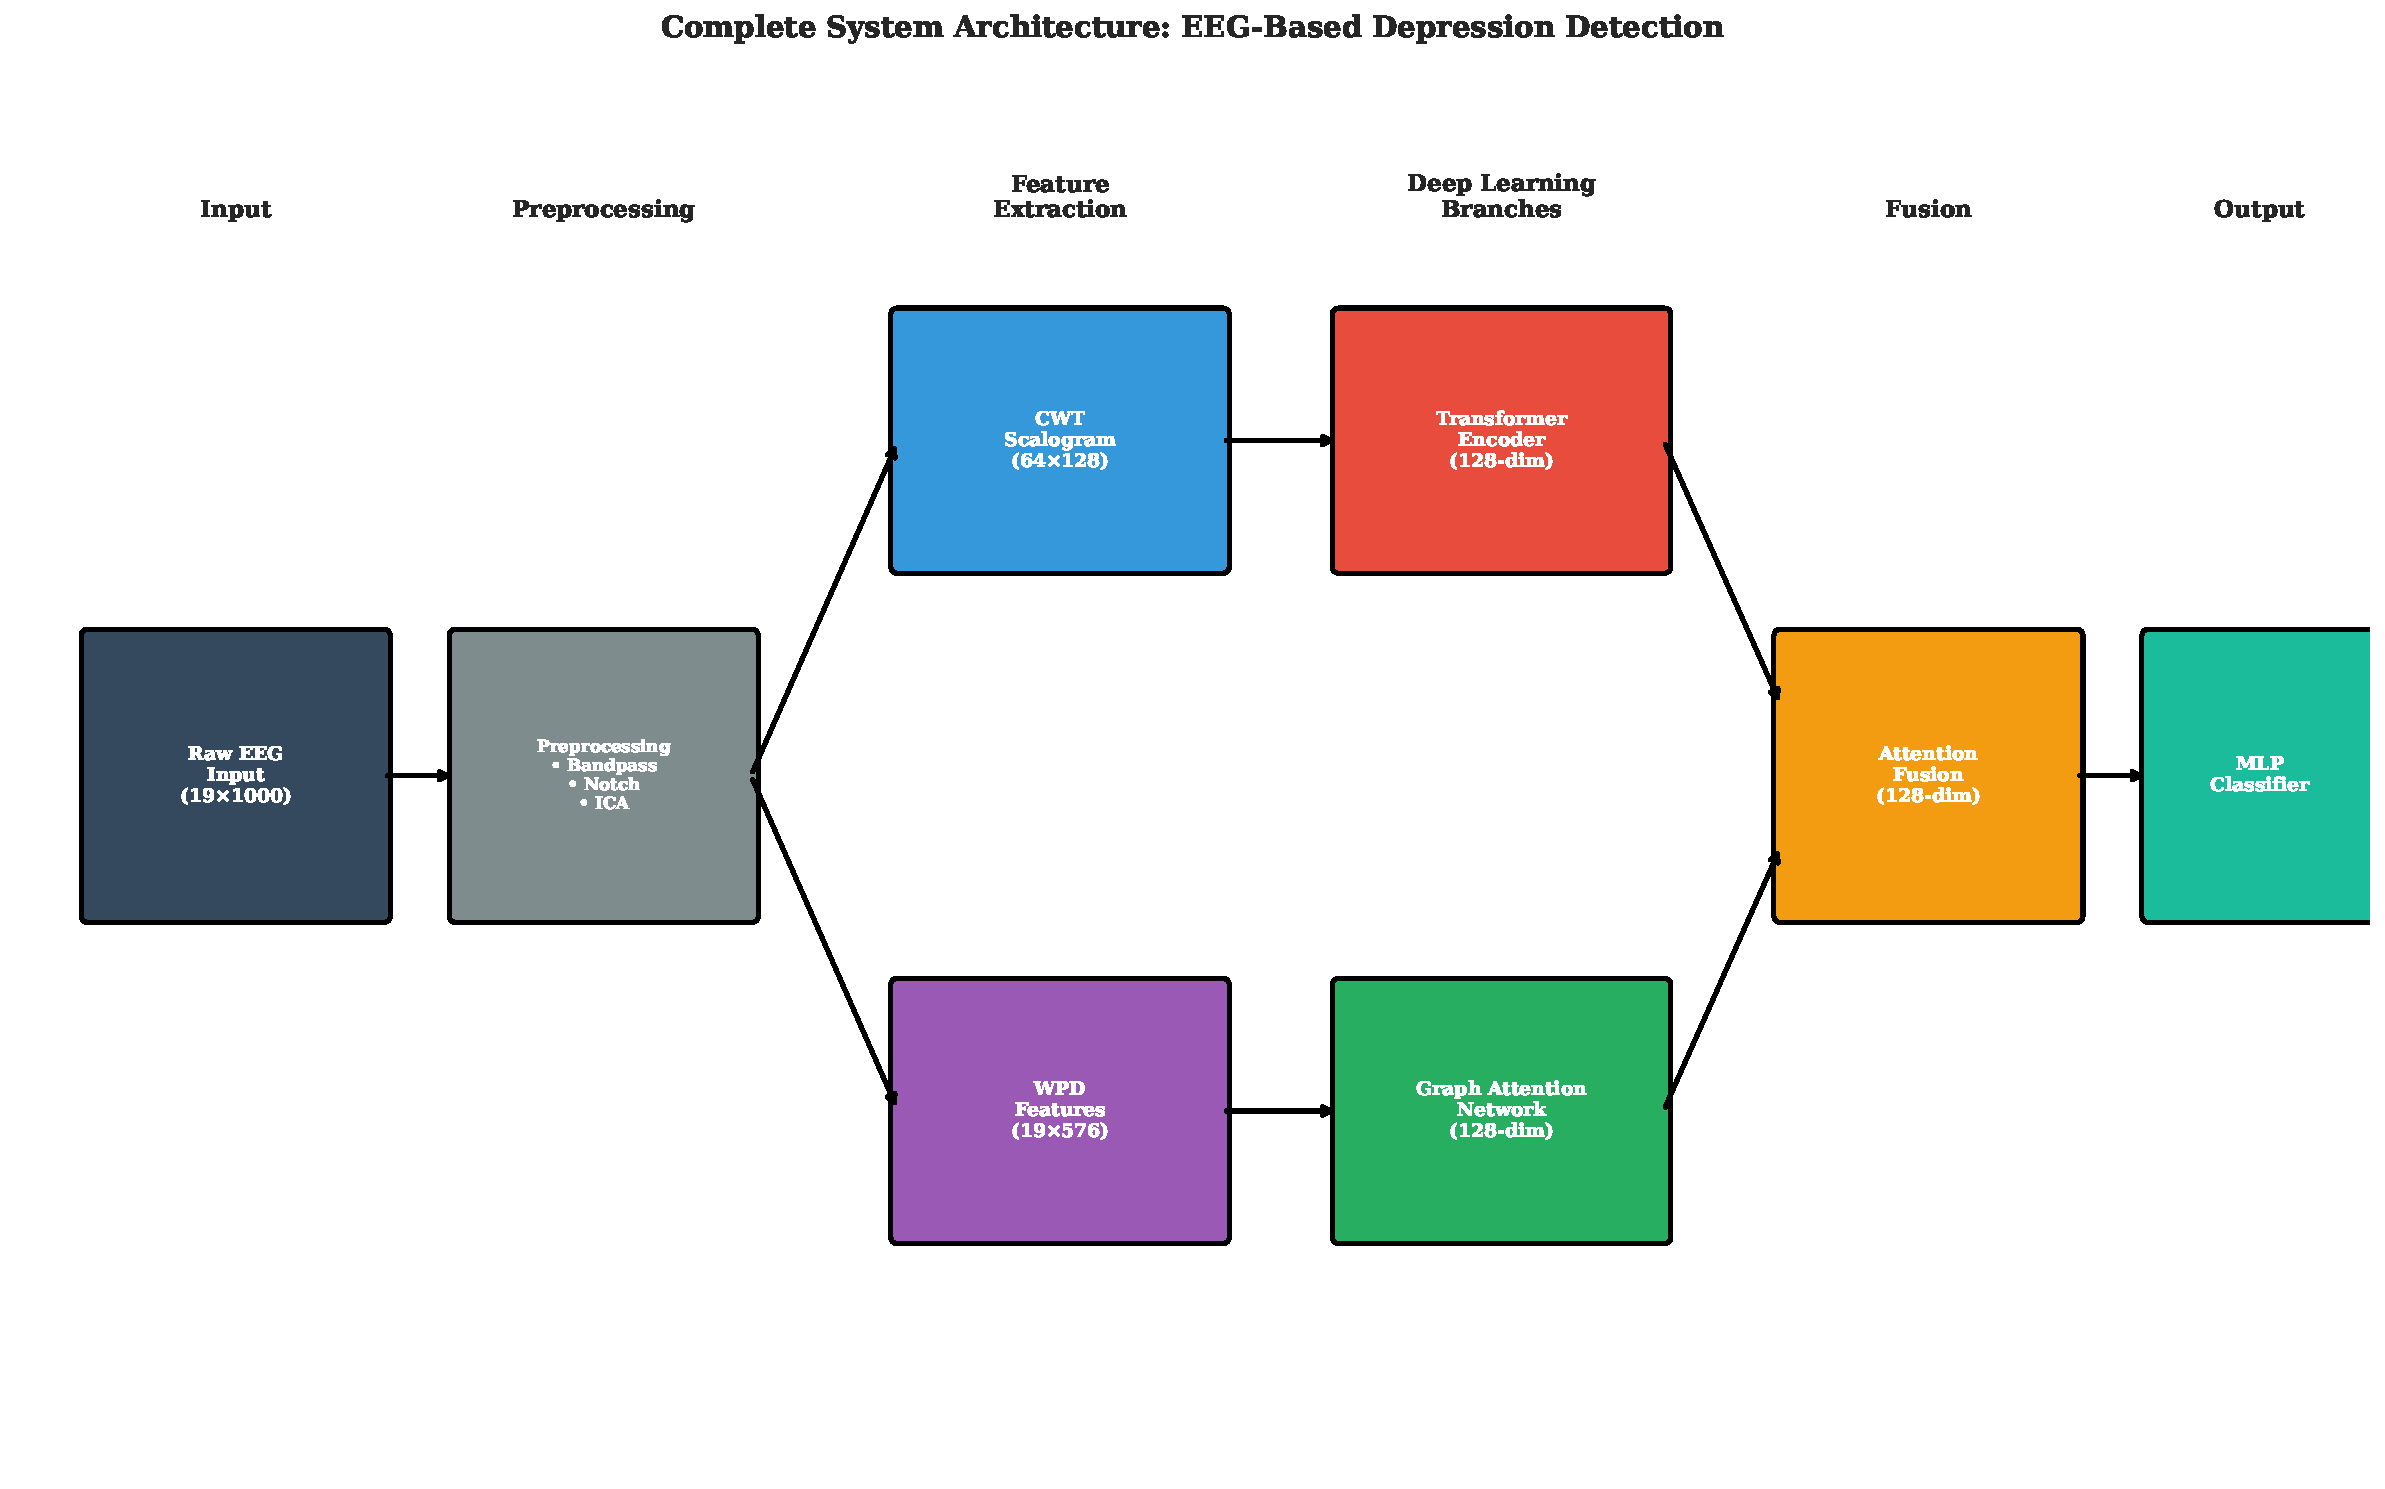
\includegraphics[width=0.95\textwidth]{figures/ch3/fig3_1_system_architecture.pdf}
    \caption{Complete system architecture showing the end-to-end processing pipeline from raw EEG signals to classification and explainability outputs.}
    \label{fig:system_architecture}
\end{figure}

\subsection{Data Flow Architecture}

At the highest level of abstraction, the system functions as a single processing unit that receives raw EEG data from the dataset repository and produces classification results with accompanying explainability reports for the clinician or researcher. The external entities interacting with the system are the EEG Dataset, which serves as the data source providing raw recordings, and the User who receives the processed outputs including depression probability scores, confidence metrics, and biomarker-level interpretations.

Decomposing the system reveals four major processing stages that operate sequentially on the data. The Data Preprocessing stage receives raw EEG signals and produces filtered, segmented epochs stored in an intermediate data structure. The Feature Extraction stage transforms these epochs into both WPD feature vectors and CWT scalograms, which may be cached for efficiency during repeated training runs. The Model Inference stage loads trained model weights and processes the extracted features through the dual-branch architecture to produce classification predictions. Finally, the Explainability Analysis stage computes attribution maps and concept scores that explain the model's decision-making process.

\section{METHODOLOGY}

\subsection{Data Preprocessing}

The preprocessing pipeline transforms raw EEG signals into clean, standardized epochs suitable for feature extraction. This transformation is critical because raw EEG recordings contain various artifacts and noise sources that would confound the classification task if not properly addressed. The preprocessing stages are applied sequentially, with each step building on the output of the previous stage to progressively refine the signal quality.

\begin{figure}[H]
    \centering
    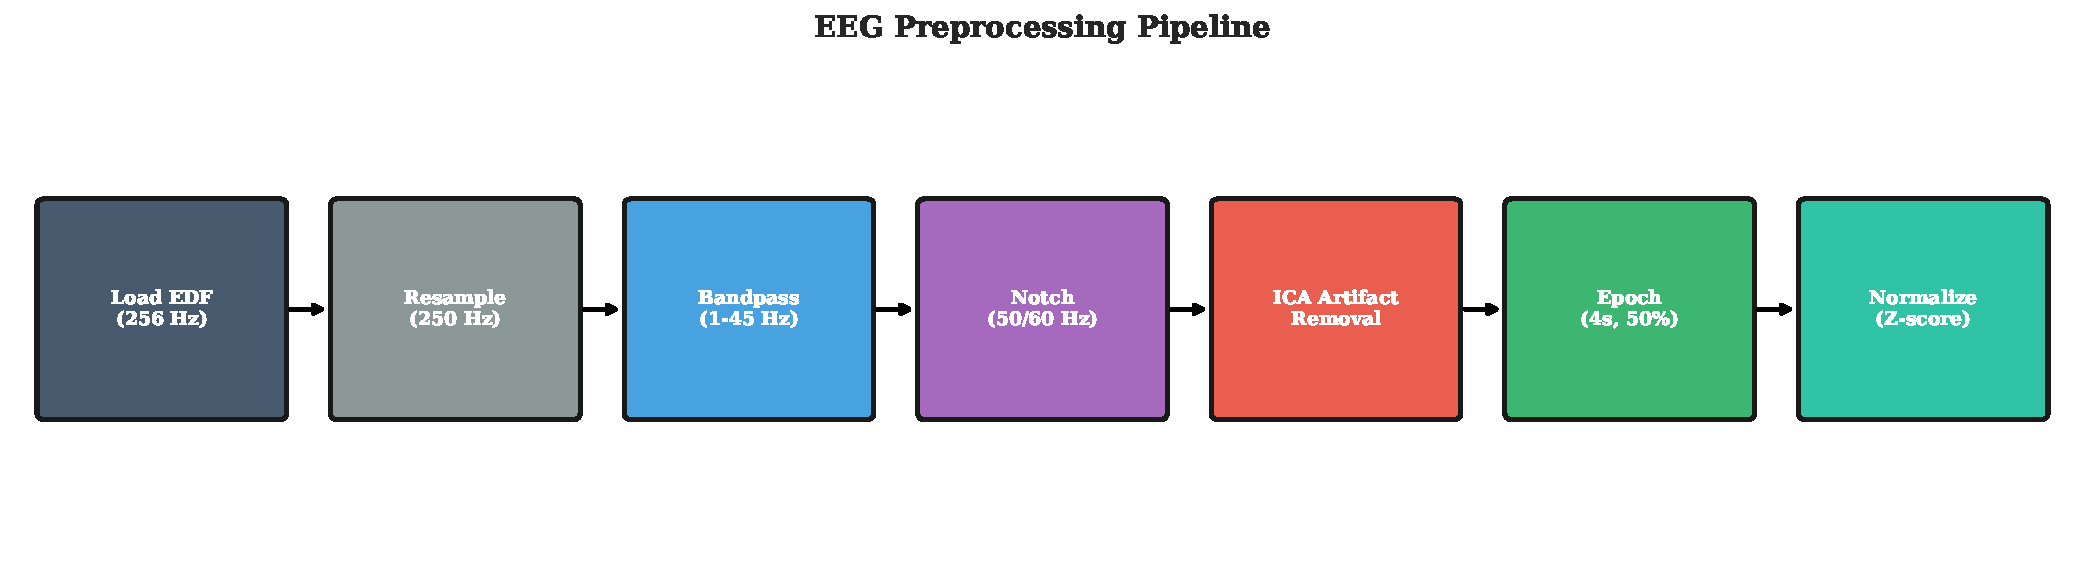
\includegraphics[width=0.95\textwidth]{figures/ch3/fig3_4_preprocessing.pdf}
    \caption{Preprocessing pipeline flowchart showing sequential signal processing stages.}
    \label{fig:preprocessing}
\end{figure}

\subsubsection{Filtering Operations}

The filtering stage applies two types of frequency-selective filters to remove unwanted signal components while preserving the neural activity of interest. A bandpass filter with cutoff frequencies of 1 Hz and 45 Hz removes both low-frequency drift and high-frequency noise that fall outside the range of standard EEG frequency bands. This filter is implemented as a Finite Impulse Response (FIR) filter with order 101, which provides linear phase characteristics that preserve the temporal relationships within the signal. The 1 Hz lower cutoff removes DC offset and slow baseline drift caused by electrode polarization and movement artifacts, while the 45 Hz upper cutoff eliminates high-frequency muscle artifacts and environmental electromagnetic interference while preserving the full gamma band activity.

Following the bandpass filter, notch filters at 50 Hz and 60 Hz remove power line interference that commonly contaminates EEG recordings. The 50 Hz notch addresses the European power grid frequency, while the 60 Hz notch addresses the North American standard, ensuring the preprocessing pipeline works correctly for datasets recorded in different geographic regions. Each notch filter has a bandwidth of 2 Hz, narrow enough to precisely target the interference frequency while minimizing distortion to nearby frequency components of interest.

\subsubsection{Artifact Removal}

Independent Component Analysis using the Picard algorithm decomposes the multi-channel EEG signal into statistically independent components, enabling identification and removal of artifact sources while preserving neural signals. Ocular artifacts from eye movements and blinks produce distinctive spatial patterns with high amplitude at frontal electrodes, while muscular artifacts from facial tension or jaw clenching produce characteristic high-frequency broadband activity. The ICA algorithm separates these artifact sources from neural components based on their statistical independence.

Components identified as artifactual based on their correlation with reference EOG channels (correlation greater than 0.8) are automatically rejected, and the signal is reconstructed from the remaining components. This automated rejection procedure ensures consistent artifact removal across all subjects while avoiding the subjectivity inherent in manual artifact identification.

\subsubsection{Epoch Segmentation}

Continuous recordings are segmented into discrete epochs of 4 seconds duration, corresponding to 1000 samples at the resampled rate of 250 Hz. The 4-second epoch length represents a carefully chosen compromise between conflicting requirements. Longer epochs capture more cycles of slower rhythms such as delta (1-4 Hz) and theta (4-8 Hz), providing stable estimates of low-frequency power. However, shorter epochs yield more samples per subject, which is valuable for training data-hungry deep learning models. The 4-second duration captures approximately 4-16 cycles of delta activity and 16-32 cycles of theta activity, sufficient for reliable spectral estimation while producing approximately 150 epochs per subject.

Epochs are extracted with 50\% overlap, meaning each time point in the continuous recording contributes to two consecutive epochs except at the boundaries. This overlap increases the total number of training samples while maintaining reasonable independence between adjacent epochs. Finally, amplitude-based rejection removes epochs containing any sample exceeding 100 µV, eliminating residual artifacts that survived the ICA cleaning process.

Table \ref{tab:preprocessing_params} summarizes the complete preprocessing parameter configuration.

\begin{table}[H]
    \centering
    \small
    \caption{Preprocessing Parameters}
    \label{tab:preprocessing_params}
    \begin{tabularx}{\textwidth}{|L{3.5cm}|L{2.5cm}|X|}
        \hline
        \textbf{Parameter} & \textbf{Value} & \textbf{Justification} \\
        \hline
        Original Sampling Rate & 256 Hz & Dataset specification \\
        \hline
        Resampled Rate & 250 Hz & Convenient for epoch length \\
        \hline
        Bandpass Range & 1-45 Hz & Covers delta through gamma \\
        \hline
        Filter Type & FIR, order 101 & Linear phase, stable \\
        \hline
        Notch Frequencies & 50, 60 Hz & Power line removal \\
        \hline
        ICA Algorithm & Picard & Fast, reliable \\
        \hline
        Epoch Duration & 4 seconds & Sufficient for slow rhythms \\
        \hline
        Epoch Overlap & 50\% & Balance data quantity and independence \\
        \hline
        Amplitude Threshold & 100 $\mu$V & Artifact rejection \\
        \hline
    \end{tabularx}
\end{table}

\subsection{Feature Extraction}

The system extracts two complementary feature types that capture different aspects of the EEG signal. Wavelet Packet Decomposition features provide fine-grained spectral analysis with 576 features per channel, serving as node attributes for the Graph Attention Network branch. Continuous Wavelet Transform scalograms provide two-dimensional time-frequency representations that serve as input to the Vision Transformer branch. This dual-feature approach ensures that both branches receive inputs optimized for their respective architectures.

\subsubsection{Wavelet Packet Decomposition (WPD)}

Wavelet Packet Decomposition extends the standard discrete wavelet transform by recursively decomposing both approximation and detail coefficients at each level, providing uniform frequency resolution across the entire spectrum. Unlike the standard DWT which only decomposes the low-frequency approximation coefficients, WPD treats approximation and detail coefficients symmetrically, yielding a complete binary tree of frequency subbands.

\begin{figure}[H]
    \centering
    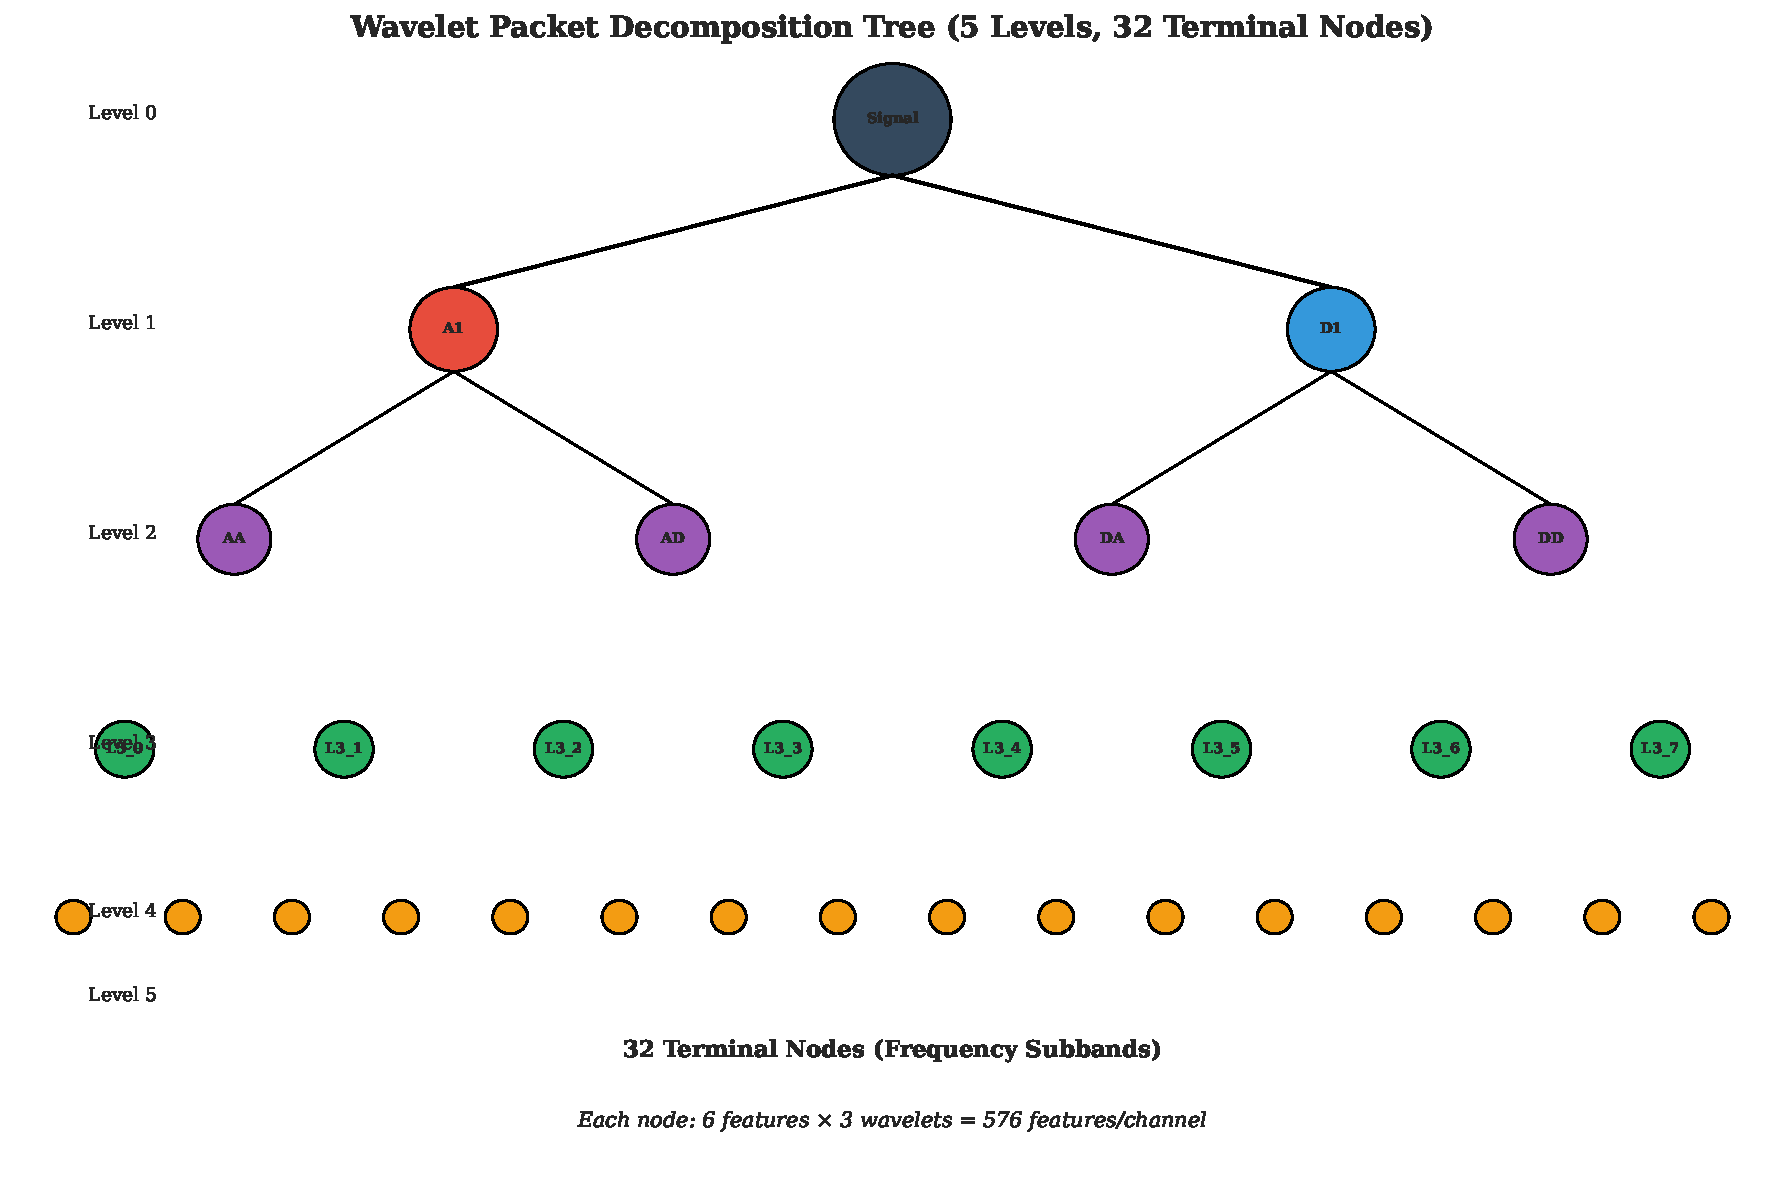
\includegraphics[width=0.95\textwidth]{figures/ch3/fig3_5_wpd_tree.pdf}
    \caption{Wavelet Packet Decomposition tree showing 5-level decomposition into 32 frequency subbands.}
    \label{fig:wpd_tree}
\end{figure}

The multi-wavelet approach employed in this system uses three complementary wavelet families rather than a single wavelet, capturing different signal characteristics through their distinct mathematical properties. The Daubechies-4 (db4) wavelet offers good time-frequency localization with a waveform shape similar to neural transients, making it well-suited for detecting sharp features in EEG signals. The Symlet-5 (sym5) wavelet provides near-symmetric filter coefficients with smooth oscillatory characteristics, reducing boundary effects at epoch edges and capturing sustained rhythmic activity. The Coiflet-3 (coif3) wavelet offers excellent symmetry with high-order vanishing moments, enabling accurate representation of polynomial trends and slowly-varying signal components.

For each of the 32 terminal nodes in the WPD tree, six statistical features are computed to characterize the coefficient distribution. Energy, computed as the sum of squared coefficients, measures the total power in each frequency subband and directly relates to traditional spectral power measures. Shannon entropy quantifies signal complexity and irregularity, with higher values indicating more random or unpredictable coefficient distributions. Log energy entropy provides an alternative complexity measure with different sensitivity characteristics. The mean captures any DC offset in the coefficient distribution, while standard deviation measures the variability around that mean. Skewness, the third standardized moment, characterizes the asymmetry of the coefficient distribution.

The total feature dimensionality per channel is computed as the product of three wavelets, 32 terminal nodes, and 6 features, yielding 576 features per channel. With 19 EEG channels, the complete WPD feature vector contains 10,944 elements, providing a rich spectral representation that captures fine-grained frequency information across the entire EEG spectrum.

\begin{table}[H]
    \centering
    \small
    \caption{WPD Feature Extraction Parameters}
    \label{tab:wpd_params}
    \begin{tabularx}{\textwidth}{|L{3.5cm}|L{3cm}|X|}
        \hline
        \textbf{Parameter} & \textbf{Value} & \textbf{Description} \\
        \hline
        Wavelet Families & db4, sym5, coif3 & Complementary characteristics \\
        \hline
        Decomposition Level & 5 & Yields 32 terminal nodes \\
        \hline
        Terminal Nodes & 32 per wavelet & Frequency resolution $\approx$ 3.9 Hz \\
        \hline
        Features per Node & 6 & Energy, entropy, statistics \\
        \hline
        Features per Channel & 576 & 3 $\times$ 32 $\times$ 6 \\
        \hline
        Total Features & 10,944 & 19 channels $\times$ 576 features \\
        \hline
    \end{tabularx}
\end{table}

\subsubsection{Continuous Wavelet Transform (CWT)}

The Continuous Wavelet Transform generates a two-dimensional time-frequency representation called a scalogram that encodes how the spectral content of the signal evolves over time. Unlike the discrete decomposition provided by WPD, CWT computes wavelet coefficients at all scales and time points, producing a dense image-like representation ideal for processing with convolutional or attention-based architectures.

\begin{figure}[H]
    \centering
    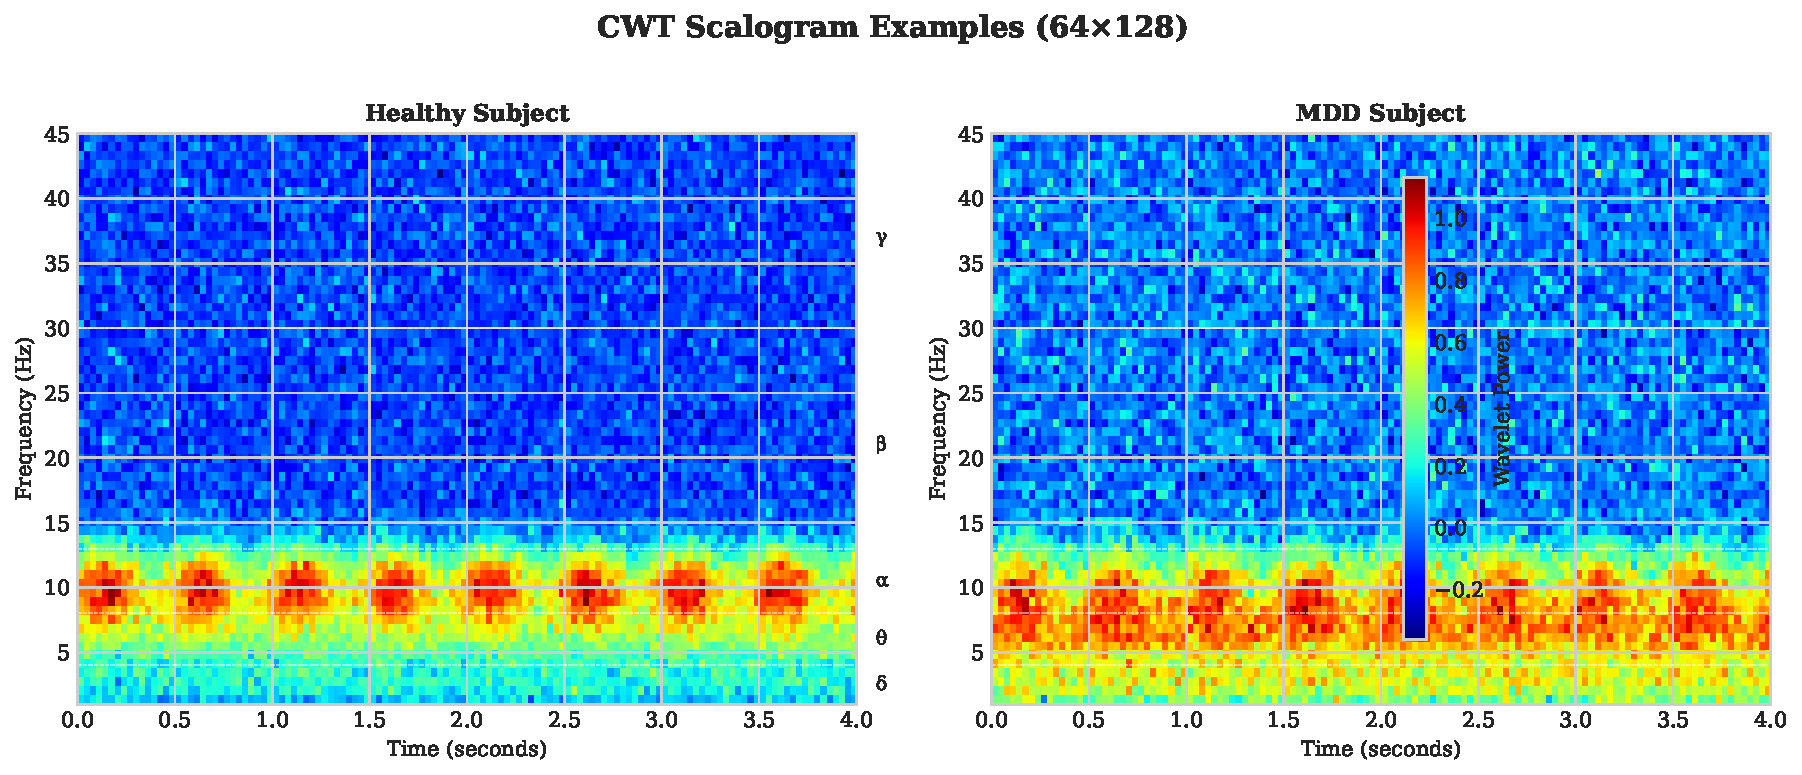
\includegraphics[width=0.85\textwidth]{figures/ch3/fig3_6_cwt_scalogram.pdf}
    \caption{Example CWT scalogram showing time-frequency representation of a 4-second EEG epoch. Horizontal bands indicate dominant frequency components; vertical patterns show temporal dynamics.}
    \label{fig:cwt_scalogram}
\end{figure}

The Complex Morlet wavelet with bandwidth parameter 1.5 and center frequency 1.0 serves as the analyzing wavelet, providing an excellent balance between time and frequency resolution for EEG analysis. The complex-valued wavelet yields both magnitude and phase information, though for the current implementation only magnitude is used. The output scalogram spans frequencies from 1 Hz to 45 Hz using 64 logarithmically-spaced frequency bins, capturing the full range of clinically relevant EEG activity from delta through gamma bands. The temporal dimension contains 128 time points spanning the 4-second epoch, yielding a final scalogram shape of 64 rows (frequency) by 128 columns (time) per channel. For computational efficiency, the scalograms are averaged across channels to produce a single representative time-frequency image per epoch.

\subsection{Model Architecture}

The proposed model consists of three main components that work together to produce depression classifications: the Transformer Branch processes time-frequency representations, the GNN Branch processes spatial electrode relationships, and the Attention-Based Fusion module combines their outputs.

\subsubsection{Transformer Branch}

The Transformer Branch processes CWT scalograms using a Vision Transformer architecture adapted for time-frequency analysis of EEG signals. The Vision Transformer, originally developed for image classification, treats two-dimensional inputs as sequences of patches and applies self-attention to learn global dependencies between patch locations. This approach is well-suited for scalogram processing because depression-related patterns may involve interactions between distant time-frequency regions that local convolutional receptive fields would miss.

\begin{figure}[H]
    \centering
    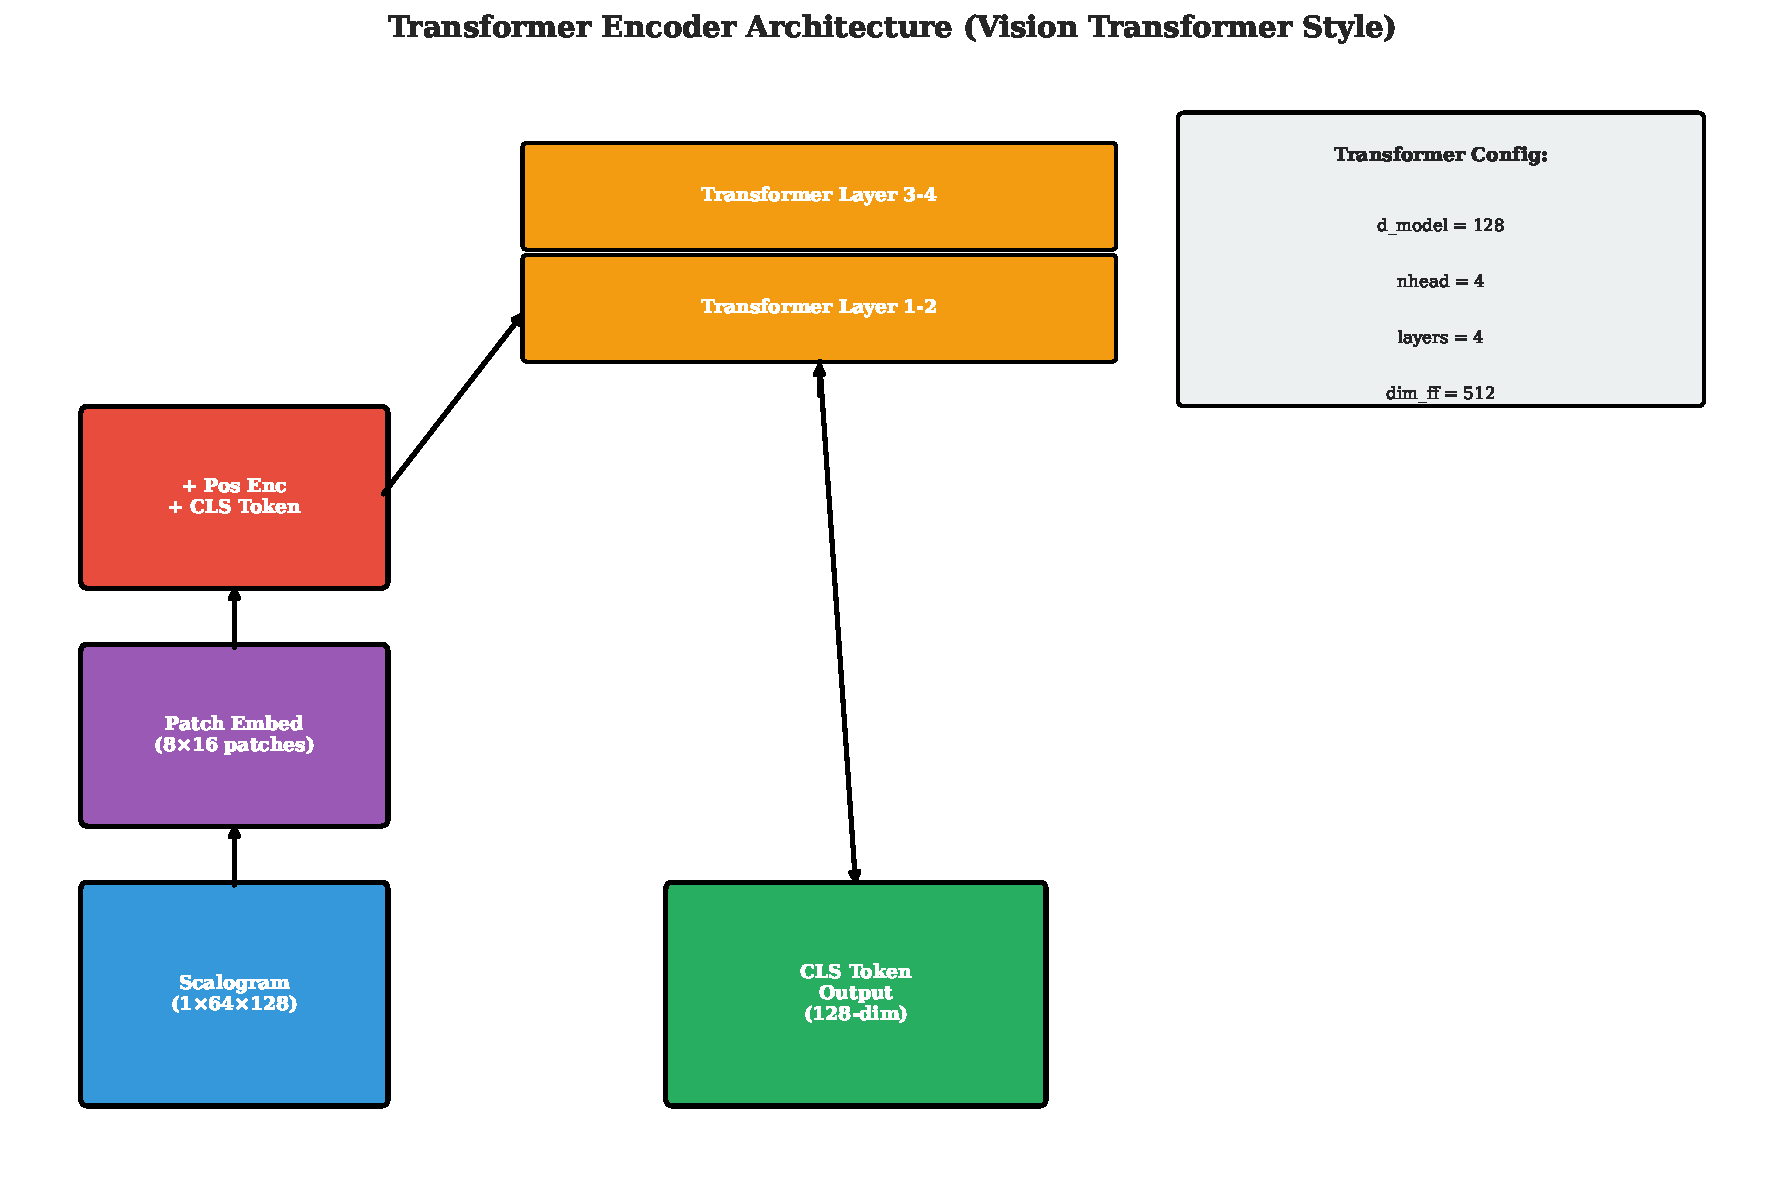
\includegraphics[width=0.95\textwidth]{figures/ch3/fig3_7_transformer.pdf}
    \caption{Transformer encoder architecture for processing CWT scalograms, following Vision Transformer design principles.}
    \label{fig:transformer_arch}
\end{figure}

The input scalogram of size 64×128 is divided into non-overlapping patches of size 8×16, yielding 64 patches that tile the complete time-frequency plane. Each patch is flattened and linearly projected to the model dimension of 128, converting the 128-element patch into a 128-dimensional embedding vector. This projection is learned during training, allowing the model to discover optimal low-dimensional representations of local time-frequency regions.

Learnable positional embeddings are added to the patch embeddings to preserve information about where each patch was located in the original scalogram. Without positional encoding, the Transformer would be permutation-invariant and unable to distinguish whether a particular pattern occurred early or late in the epoch, or in low versus high frequency regions. A learnable classification token is prepended to the sequence of patch embeddings, serving as an aggregation point that collects information from all patches through the attention mechanism.

The resulting sequence of 65 tokens (64 patches plus the CLS token) passes through four Transformer encoder layers, each containing multi-head self-attention followed by a feed-forward network with GELU activation. The self-attention mechanism with 4 heads allows each position to attend to all other positions, learning which time-frequency regions are most relevant to each other for depression detection. After processing through all encoder layers, the final representation of the CLS token serves as the 128-dimensional output of the Transformer branch.

\begin{table}[H]
    \centering
    \small
    \caption{Transformer Branch Hyperparameters}
    \label{tab:transformer_params}
    \begin{tabularx}{\textwidth}{|L{4cm}|L{2.5cm}|X|}
        \hline
        \textbf{Parameter} & \textbf{Value} & \textbf{Rationale} \\
        \hline
        Input Size & 64 $\times$ 128 & CWT scalogram dimensions \\
        \hline
        Patch Size & 8 $\times$ 16 & 64 total patches \\
        \hline
        Model Dimension (d\_model) & 128 & Memory efficient; expressive \\
        \hline
        Attention Heads & 4 & Head dimension = 32 \\
        \hline
        Encoder Layers & 4 & Sufficient depth for patterns \\
        \hline
        Feed-Forward Dimension & 512 & 4$\times$ d\_model (standard) \\
        \hline
        Dropout & 0.1 & Regularization \\
        \hline
        Activation & GELU & Smooth, works well with Transformers \\
        \hline
        Use CLS Token & True & Classification representation \\
        \hline
        Output Dimension & 128 & Matches d\_model \\
        \hline
        Parameters & 892,416 & Transformer branch total \\
        \hline
    \end{tabularx}
\end{table}

\subsubsection{GNN Branch}

The Graph Attention Network branch models spatial relationships between EEG electrodes by representing them as nodes in a graph where edges encode connectivity patterns. Unlike approaches that treat EEG channels as independent features or as a simple sequence, the GNN explicitly captures the topological structure of the electrode array and learns which inter-electrode relationships are most informative for depression detection.

\begin{figure}[H]
    \centering
    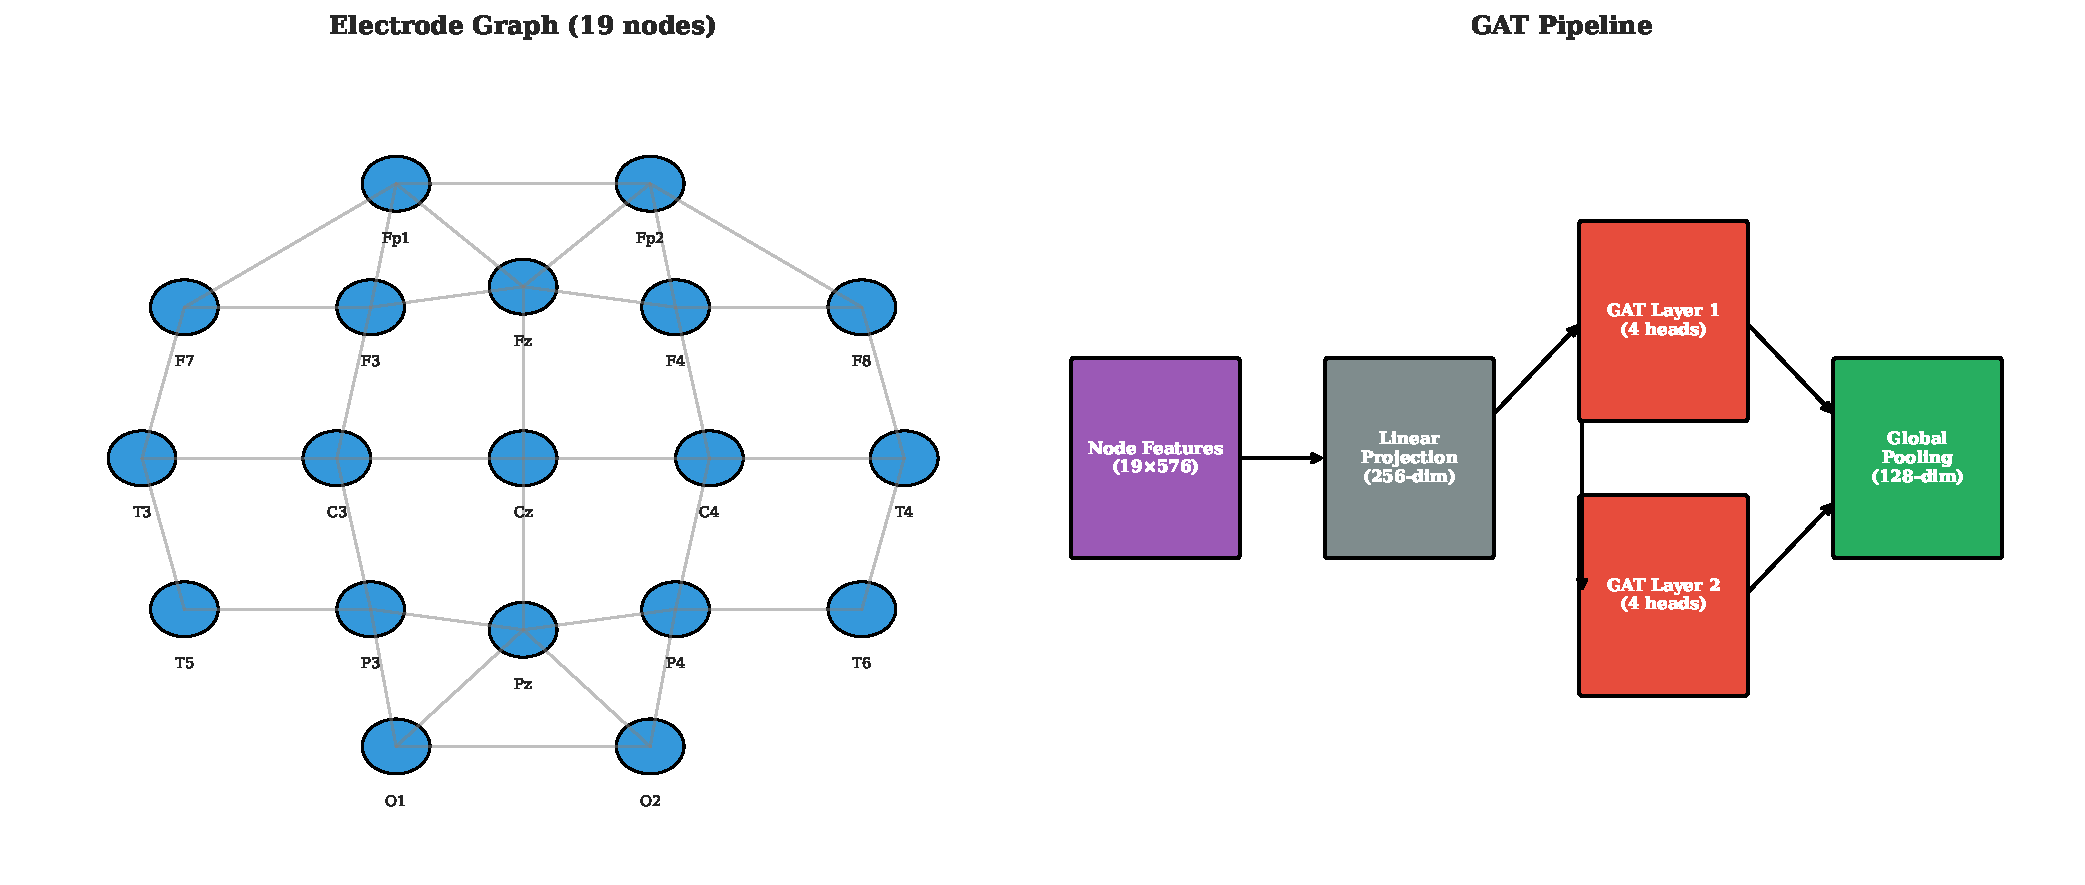
\includegraphics[width=0.95\textwidth]{figures/ch3/fig3_8_gnn.pdf}
    \caption{Graph Attention Network architecture showing electrode graph construction and message passing layers.}
    \label{fig:gnn_arch}
\end{figure}

The electrode graph is constructed using a hybrid adjacency scheme that combines spatial proximity with functional connectivity. The spatial adjacency component connects each electrode to its 6 nearest neighbors based on the three-dimensional coordinates of the 10-20 electrode positions, capturing the physical layout of the recording array. The functional adjacency component adds edges between electrode pairs whose signals show Pearson correlation exceeding 0.5, capturing data-driven connectivity patterns that may reflect underlying neural coupling. This hybrid approach ensures that both anatomically-grounded and functionally-observed relationships inform the graph structure.

Each node in the graph receives the 576-dimensional WPD feature vector computed for the corresponding electrode as its input attribute. An initial projection layer reduces this to a 256-dimensional hidden representation. Three Graph Attention convolutional layers then perform message passing, where each node aggregates information from its neighbors weighted by learned attention coefficients. The attention mechanism enables the network to focus on the most relevant connections for depression detection, providing interpretability through the learned attention weights. Multi-head attention with 4 heads allows the network to attend to different aspects of the connectivity patterns simultaneously.

After the final GAT layer, global mean pooling aggregates node representations across the entire graph into a single 128-dimensional vector, producing an output that matches the dimensionality of the Transformer branch for fusion.

\begin{table}[H]
    \centering
    \small
    \caption{GNN Branch Hyperparameters}
    \label{tab:gnn_params}
    \begin{tabularx}{\textwidth}{|L{4cm}|L{2.5cm}|X|}
        \hline
        \textbf{Parameter} & \textbf{Value} & \textbf{Rationale} \\
        \hline
        Number of Nodes & 19 & 10-20 electrode montage \\
        \hline
        Node Feature Dimension & 576 & WPD features per channel \\
        \hline
        Hidden Dimension & 256 & Intermediate representation \\
        \hline
        Output Dimension & 128 & Matches Transformer output \\
        \hline
        GAT Layers & 3 & Sufficient for 19-node graph \\
        \hline
        Attention Heads & 4 & Multi-head attention \\
        \hline
        Spatial k-neighbors & 6 & Local connectivity \\
        \hline
        Functional Threshold & 0.5 & Correlation-based edges \\
        \hline
        Dropout & 0.3 & Higher than Transformer (smaller graph) \\
        \hline
        Pooling & Global Mean & Aggregate node features \\
        \hline
        Parameters & 462,592 & GNN branch total \\
        \hline
    \end{tabularx}
\end{table}

\subsubsection{Attention-Based Fusion}

The fusion module adaptively combines the 128-dimensional feature vectors from the Transformer and GNN branches, learning to weight their contributions based on the input characteristics. Simple concatenation or averaging would treat both branches equally regardless of which provides more relevant information for a particular sample. The attention-based approach instead learns dynamic weights that can emphasize whichever modality is more informative.

The cross-attention mechanism enables each branch to attend to the other, learning which complementary features to incorporate. When the Transformer features attend to the GNN features, the model learns which spatial connectivity patterns are most relevant given the observed time-frequency characteristics. Conversely, when the GNN features attend to the Transformer features, the model learns which time-frequency patterns matter most given the spatial electrode relationships. This bidirectional attention creates a rich interaction between the two modalities.

Learned gating weights further modulate the branch contributions, computed by a small neural network that receives the concatenated branch outputs and produces a two-element softmax-normalized weight vector. These weights determine the relative contribution of each branch to the final fused representation. The output projection combines the attended features with the gated mixture, producing a 128-dimensional fused representation that proceeds to the classification head.

\subsection{Training Strategy}

\subsubsection{LOSO Cross-Validation}

Leave-One-Subject-Out cross-validation ensures honest performance evaluation by completely separating subjects between training and test sets. The protocol iterates through all 58 subjects, holding out one subject at a time as the test set while training on the remaining 57 subjects. This creates 58 independent training runs, each evaluated on a subject whose data was never seen during training.

\begin{figure}[H]
    \centering
    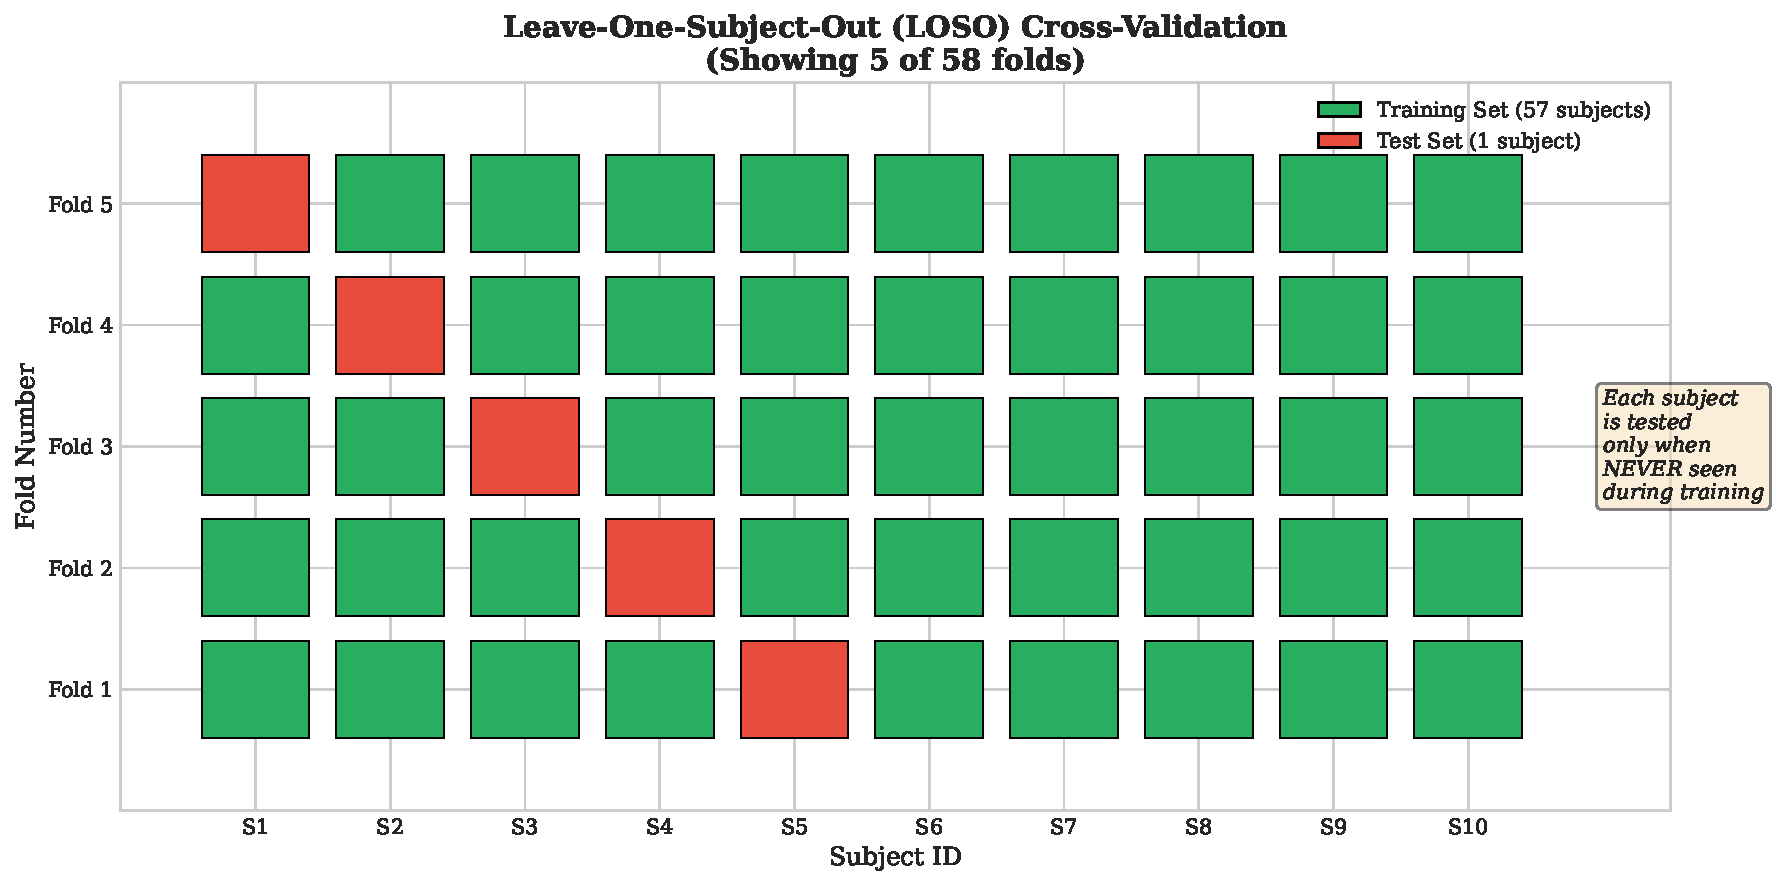
\includegraphics[width=0.9\textwidth]{figures/ch3/fig3_10_loso.pdf}
    \caption{Leave-One-Subject-Out (LOSO) cross-validation protocol ensuring each subject is tested only when completely unseen during training.}
    \label{fig:loso}
\end{figure}

For each fold, the held-out subject's epochs form the test set, while the remaining subjects are further split into training and validation sets using a 90/10 split. The model is trained from scratch with random initialization, as transfer learning between folds could introduce subtle information leakage. Training proceeds for up to 30 epochs with early stopping based on validation loss with patience of 10 epochs, preventing overfitting while allowing sufficient training when validation performance continues improving. After training completes, the model is evaluated on the test subject and predictions are saved along with ground truth labels for later aggregation.

After completing all 58 folds, the predictions are aggregated to compute final performance metrics. Subject-level accuracy is computed by majority voting across each subject's epochs, while sample-level accuracy is computed across all individual epoch predictions. Additional metrics including AUC-ROC, F1-score, precision, recall, and confusion matrix provide a comprehensive view of classification performance.

\begin{table}[H]
    \centering
    \small
    \caption{Training Configuration}
    \label{tab:training_config}
    \begin{tabularx}{\textwidth}{|L{3.5cm}|L{3cm}|X|}
        \hline
        \textbf{Parameter} & \textbf{Value} & \textbf{Description} \\
        \hline
        Cross-Validation & LOSO & 58 folds (one per subject) \\
        \hline
        Epochs per Fold & 30 & With early stopping \\
        \hline
        Batch Size & 16 & Limited by GPU memory \\
        \hline
        Effective Batch & 32 & Via gradient accumulation (2 steps) \\
        \hline
        Optimizer & AdamW & Decoupled weight decay \\
        \hline
        Learning Rate & 1e-4 & Conservative for small dataset \\
        \hline
        Weight Decay & 0.01 & L2 regularization \\
        \hline
        Scheduler & CosineAnnealing & With warm restarts \\
        \hline
        Early Stopping & Patience 10 & Prevent overfitting \\
        \hline
        Mixed Precision & FP16 & Memory efficiency \\
        \hline
        Gradient Clipping & 1.0 & Training stability \\
        \hline
    \end{tabularx}
\end{table}

\section{MODULE DESCRIPTION}

The system is organized into nine modules with clearly defined responsibilities and interfaces. Table \ref{tab:modules} describes each module with its input and output specifications, enabling independent development, testing, and maintenance of system components.

\begin{table}[H]
    \centering
    \small
    \caption{Module Input/Output Specifications}
    \label{tab:modules}
    \begin{tabularx}{\textwidth}{|L{2cm}|L{3cm}|L{3cm}|X|}
        \hline
        \textbf{Module} & \textbf{Input} & \textbf{Output} & \textbf{Function} \\
        \hline
        M1: Data Loading & EDF file paths & Raw EEG arrays (19, N) & Load multi-channel recordings \\
        \hline
        M2: Preprocessing & Raw EEG (19, N) & Filtered epochs (B, 19, 1000) & Filter, segment, normalize \\
        \hline
        M3: WPD Extraction & Epochs (B, 19, 1000) & WPD features (B, 19, 576) & Multi-wavelet decomposition \\
        \hline
        M4: CWT Generation & Epochs (B, 19, 1000) & Scalograms (B, 1, 64, 128) & Time-frequency transform \\
        \hline
        M5: Transformer & Scalogram (B, 1, 64, 128) & Features (B, 128) & Time-frequency encoding \\
        \hline
        M6: GNN & WPD (B, 19, 576), Graph & Features (B, 128) & Spatial encoding \\
        \hline
        M7: Fusion & Trans (B, 128), GNN (B, 128) & Fused (B, 128) & Feature combination \\
        \hline
        M8: Classifier & Fused (B, 128) & Probability (B, 1) & Depression prediction \\
        \hline
        M9: Explainability & Model, Input & Attributions, Scores & IG, LRP, TCAV \\
        \hline
    \end{tabularx}
\end{table}

The data flow between modules follows a logical progression from raw data to final predictions. The Data Loading module (M1) parses EDF files and extracts multi-channel time series. The Preprocessing module (M2) applies filtering and segmentation to produce standardized epochs. The WPD Extraction (M3) and CWT Generation (M4) modules operate in parallel on the preprocessed epochs, producing features for their respective model branches. The Transformer (M5) and GNN (M6) modules encode their inputs into fixed-dimensional representations. The Fusion module (M7) combines branch outputs, and the Classifier (M8) produces final predictions. The Explainability module (M9) operates after training to analyze model decision-making through gradient-based and concept-based methods.

\section{DATA DESIGN}

\subsection{Dataset Specification}

The system uses the Figshare MDD EEG Dataset, a publicly available resource specifically curated for depression research. This dataset provides resting-state EEG recordings from both Major Depressive Disorder patients and healthy control subjects, recorded under standardized conditions that ensure comparability across subjects.

The dataset is organized into two subdirectories corresponding to the two diagnostic categories. The MDD directory contains 29 recordings from patients diagnosed with Major Depressive Disorder according to DSM-5 criteria, while the Healthy directory contains 29 recordings from control subjects with no psychiatric history. Each recording file follows a standardized naming convention indicating the diagnostic group, subject number, and recording condition (Eyes Closed). The Eyes Closed resting state condition was chosen because it minimizes visual processing artifacts while maintaining a standardized cognitive state across subjects.

\subsection{Dataset Demographics}

The dataset includes balanced representation of both diagnostic groups with matched demographic characteristics to minimize confounding variables. Table \ref{tab:demographics} presents the demographic characteristics of the participant groups.

\begin{table}[H]
    \centering
    \small
    \caption{Dataset Demographics}
    \label{tab:demographics}
    \begin{tabularx}{\textwidth}{|X|c|c|}
        \hline
        \textbf{Characteristic} & \textbf{MDD Group} & \textbf{Healthy Control} \\
        \hline
        Number of Subjects & 29 & 29 \\
        \hline
        Age Range & 18-65 years & 18-65 years \\
        \hline
        Gender & Mixed & Mixed \\
        \hline
        Diagnosis & DSM-5 MDD criteria & No psychiatric history \\
        \hline
        Medication Status & Medication-free or stable & None \\
        \hline
    \end{tabularx}
\end{table}

\subsection{Recording Parameters}

All recordings follow the International 10-20 System for electrode placement, using 19 standard electrode positions that provide comprehensive coverage of the scalp surface. Table \ref{tab:recording_params} specifies the complete recording parameters.

\begin{table}[H]
    \centering
    \small
    \caption{EEG Recording Parameters}
    \label{tab:recording_params}
    \begin{tabularx}{\textwidth}{|L{3.5cm}|X|}
        \hline
        \textbf{Parameter} & \textbf{Value} \\
        \hline
        Electrodes & 19 (International 10-20 System) \\
        \hline
        Channel Names & Fp1, Fp2, F7, F3, Fz, F4, F8, T3, C3, Cz, C4, T4, T5, P3, Pz, P4, T6, O1, O2 \\
        \hline
        Sampling Rate & 256 Hz (original), resampled to 250 Hz \\
        \hline
        Reference & Linked ears \\
        \hline
        Recording Duration & $\approx$ 5 minutes per subject \\
        \hline
        Condition & Eyes Closed (EC) resting state \\
        \hline
        File Format & EDF (European Data Format) \\
        \hline
    \end{tabularx}
\end{table}

The 19 electrodes span five anatomical regions: frontal electrodes (Fp1, Fp2, F7, F3, Fz, F4, F8) over the prefrontal and frontal cortex, central electrodes (C3, Cz, C4) over the motor cortex, temporal electrodes (T3, T4, T5, T6) over the temporal lobes, parietal electrodes (P3, Pz, P4) over the parietal cortex, and occipital electrodes (O1, O2) over the visual cortex. This standardized montage enables direct comparison with other studies and aligns with the established literature on depression-related EEG biomarkers.

\subsection{Class Distribution}

After preprocessing, the dataset yields a nearly balanced distribution of epochs between the two classes. Table \ref{tab:class_distribution} presents the final dataset statistics.

\begin{table}[H]
    \centering
    \small
    \caption{Final Dataset Class Distribution}
    \label{tab:class_distribution}
    \begin{tabularx}{\textwidth}{|X|r|r|}
        \hline
        \textbf{Metric} & \textbf{Value} & \textbf{Percentage} \\
        \hline
        Total Subjects & 58 & 100\% \\
        \hline
        MDD Subjects & 29 & 50\% \\
        \hline
        Healthy Subjects & 29 & 50\% \\
        \hline
        Total Epochs & 8,620 & 100\% \\
        \hline
        MDD Epochs & 4,373 & 50.7\% \\
        \hline
        Healthy Epochs & 4,247 & 49.3\% \\
        \hline
        Average Epochs/Subject & $\approx$ 148 & --- \\
        \hline
        Min Epochs/Subject & 89 & --- \\
        \hline
        Max Epochs/Subject & 196 & --- \\
        \hline
    \end{tabularx}
\end{table}

The near-perfect class balance (50.7\% MDD versus 49.3\% Healthy) at the epoch level eliminates the need for class weighting or oversampling techniques that could introduce bias or complicate training dynamics. The subject-level balance is exact with 29 subjects in each group. The variation in epochs per subject (ranging from 89 to 196) reflects differences in recording duration and the number of epochs rejected during artifact removal, but this variation does not significantly impact class balance due to the large number of subjects.



% Chapter 4: System Implementation
% ============================================================================
% CHAPTER 4: SYSTEM IMPLEMENTATION
% ============================================================================

\chapter{SYSTEM IMPLEMENTATION}

\section{MODULE IMPLEMENTATION}

This section describes the implementation of key system modules with relevant code excerpts and explanations, providing sufficient detail for reproducibility while focusing on the most architecturally significant components.

\subsection{Development Environment}

The system is implemented in Python using modern deep learning frameworks and specialized libraries for EEG processing. Table \ref{tab:packages} lists the primary packages and their purposes. PyTorch serves as the core deep learning framework, providing automatic differentiation, GPU acceleration, and a rich ecosystem of model building blocks. PyTorch Geometric extends PyTorch with efficient implementations of graph neural network operations, including the Graph Attention layers used in the GNN branch. MNE-Python handles EEG-specific data loading and preprocessing, providing robust implementations of filtering, artifact rejection, and epoch extraction that follow established best practices in the neuroimaging community.

\begin{table}[H]
    \centering
    \small
    \caption{Primary Python Packages and Versions}
    \label{tab:packages}
    \begin{tabularx}{\textwidth}{|L{3.5cm}|L{2cm}|X|}
        \hline
        \textbf{Package} & \textbf{Version} & \textbf{Purpose} \\
        \hline
        Python & 3.10+ & Programming language \\
        \hline
        PyTorch & 2.0+ & Deep learning framework \\
        \hline
        PyTorch Geometric & 2.3+ & Graph neural network operations \\
        \hline
        MNE-Python & 1.5+ & EEG data loading and preprocessing \\
        \hline
        PyWavelets & 1.4+ & Wavelet transforms (WPD, CWT) \\
        \hline
        NumPy & 1.24+ & Numerical computing \\
        \hline
        SciPy & 1.10+ & Signal processing utilities \\
        \hline
        scikit-learn & 1.3+ & Metrics and utilities \\
        \hline
        Captum & 0.6+ & Model interpretability (IG, LRP) \\
        \hline
        Matplotlib & 3.7+ & Visualization \\
        \hline
        tqdm & 4.65+ & Progress bars \\
        \hline
    \end{tabularx}
\end{table}

\subsection{Transformer Encoder Implementation}

The Transformer encoder processes CWT scalograms using patch-based tokenization followed by self-attention, adapting the Vision Transformer architecture for time-frequency analysis of EEG signals. The implementation begins with a patch embedding layer that divides the input scalogram into a grid of non-overlapping patches and projects each patch to the model dimension. A learnable classification token and positional encodings are added before the sequence passes through multiple Transformer encoder layers.

\begin{lstlisting}[language=Python, caption={Transformer Encoder Core Structure (transformer\_encoder.py)}]
class EEGTransformerEncoder(nn.Module):
    def __init__(self, img_size=(64, 128), patch_size=(8, 16),
                 d_model=128, nhead=4, num_layers=4):
        super().__init__()

        # Patch embedding: convert scalogram to token sequence
        self.patch_embed = PatchEmbedding(
            img_size=img_size, patch_size=patch_size,
            in_channels=1, embed_dim=d_model
        )

        # Learnable CLS token for classification
        self.cls_token = nn.Parameter(torch.randn(1, 1, d_model) * 0.02)

        # Positional encoding (learnable)
        n_patches = self.patch_embed.n_patches + 1  # +1 for CLS
        self.pos_encoding = nn.Parameter(
            torch.randn(1, n_patches, d_model) * 0.02
        )

        # Transformer encoder layers
        encoder_layer = nn.TransformerEncoderLayer(
            d_model=d_model, nhead=nhead, dim_feedforward=512,
            dropout=0.1, activation='gelu', batch_first=True
        )
        self.transformer = nn.TransformerEncoder(
            encoder_layer, num_layers=num_layers
        )

    def forward(self, x):
        # x: (B, 1, 64, 128) - scalogram
        B = x.shape[0]

        # Patch embedding: (B, 64, 128)
        x = self.patch_embed(x)

        # Prepend CLS token
        cls = self.cls_token.expand(B, -1, -1)
        x = torch.cat([cls, x], dim=1)

        # Add positional encoding
        x = x + self.pos_encoding

        # Transformer forward
        x = self.transformer(x)

        # Return CLS token output
        return x[:, 0]  # (B, 128)
\end{lstlisting}

The implementation leverages PyTorch's built-in TransformerEncoderLayer, which encapsulates multi-head self-attention followed by a position-wise feed-forward network with layer normalization and residual connections. The patch embedding layer is implemented as a convolutional layer with kernel size and stride equal to the patch size, efficiently extracting and projecting all patches in a single operation. The CLS token and positional encodings are initialized with small random values (scaled by 0.02) following best practices from the Vision Transformer literature.

\subsection{Graph Attention Network Implementation}

The GNN branch models electrode spatial relationships using multi-head attention over the electrode graph, learning which connections between electrodes are most informative for depression detection. The implementation uses the GATConv layer from PyTorch Geometric, which implements the Graph Attention mechanism with efficient sparse matrix operations.

\begin{lstlisting}[language=Python, caption={GNN Encoder Core Structure (gnn\_encoder.py)}]
class EEGGraphAttentionNetwork(nn.Module):
    def __init__(self, in_features=576, hidden_dim=256,
                 out_dim=128, num_heads=4):
        super().__init__()

        # Input projection
        self.input_proj = nn.Linear(in_features, hidden_dim)

        # Graph Attention layers
        self.gat1 = GATConv(hidden_dim, hidden_dim // num_heads,
                           heads=num_heads, dropout=0.3)
        self.gat2 = GATConv(hidden_dim, hidden_dim // num_heads,
                           heads=num_heads, dropout=0.3)
        self.gat3 = GATConv(hidden_dim, out_dim,
                           heads=1, concat=False, dropout=0.3)

        # Layer normalization
        self.norm1 = nn.LayerNorm(hidden_dim)
        self.norm2 = nn.LayerNorm(hidden_dim)

    def forward(self, x, edge_index, batch):
        # x: (N_total, 576) node features
        # edge_index: (2, E) graph edges

        # Project input
        x = F.relu(self.input_proj(x))

        # GAT layers with residual connections
        x = x + F.elu(self.gat1(x, edge_index))
        x = self.norm1(x)

        x = x + F.elu(self.gat2(x, edge_index))
        x = self.norm2(x)

        x = self.gat3(x, edge_index)

        # Global mean pooling over nodes
        x = global_mean_pool(x, batch)  # (B, 128)

        return x
\end{lstlisting}

The architecture employs three GAT layers with residual connections and layer normalization between layers, following modern graph neural network design practices. The first two layers use multi-head attention with head outputs concatenated, while the final layer uses a single head with output dimension matching the target feature size. Dropout of 0.3 is applied within the GAT layers for regularization. Global mean pooling aggregates node representations into a single graph-level representation, producing a fixed-dimensional output regardless of the number of nodes.

\subsection{Attention Fusion Implementation}

The fusion module combines features from both branches using cross-attention and gating mechanisms, enabling adaptive weighting of branch contributions based on input characteristics. The implementation uses PyTorch's MultiheadAttention for the cross-attention operations, providing efficient computation with optional flash attention on supported hardware.

\begin{lstlisting}[language=Python, caption={Attention Fusion Mechanism (attention\_fusion.py)}]
class AttentionBasedFusion(nn.Module):
    def __init__(self, dim=128):
        super().__init__()

        # Cross-attention: Transformer attends to GNN
        self.cross_attn_t2g = nn.MultiheadAttention(
            dim, num_heads=4, batch_first=True
        )
        # Cross-attention: GNN attends to Transformer
        self.cross_attn_g2t = nn.MultiheadAttention(
            dim, num_heads=4, batch_first=True
        )

        # Gating mechanism
        self.gate = nn.Sequential(
            nn.Linear(dim * 2, dim),
            nn.ReLU(),
            nn.Linear(dim, 2),
            nn.Softmax(dim=-1)
        )

        # Output projection
        self.output_proj = nn.Linear(dim * 2, dim)

    def forward(self, trans_feat, gnn_feat):
        # Expand for attention (add sequence dim)
        t = trans_feat.unsqueeze(1)  # (B, 1, 128)
        g = gnn_feat.unsqueeze(1)    # (B, 1, 128)

        # Cross-attention
        t_attended, _ = self.cross_attn_t2g(t, g, g)
        g_attended, _ = self.cross_attn_g2t(g, t, t)

        # Squeeze back
        t_attended = t_attended.squeeze(1)
        g_attended = g_attended.squeeze(1)

        # Compute gate weights
        concat = torch.cat([trans_feat, gnn_feat], dim=-1)
        gate_weights = self.gate(concat)  # (B, 2)

        # Weighted combination
        fused = (gate_weights[:, 0:1] * t_attended +
                 gate_weights[:, 1:2] * g_attended)

        # Final projection
        output = self.output_proj(concat) + fused

        return output  # (B, 128)
\end{lstlisting}

The cross-attention mechanism allows each branch to query the other, learning which complementary features are most relevant. The gating network receives the concatenated branch features and produces a two-element softmax-normalized weight vector that determines the relative contribution of each attended representation. The final output combines the projected concatenation with the gated attended features through a residual connection, ensuring that both the original and attended information contribute to the fused representation.

\subsection{Model Parameters Summary}

The complete model contains approximately 1.55 million trainable parameters distributed across the four main components. Table \ref{tab:model_params} presents the parameter counts, revealing that the Transformer branch accounts for the majority of parameters due to its deeper architecture and larger embedding dimensions. The GNN branch is more parameter-efficient due to the smaller graph size (19 nodes) and shared message passing operations. The fusion and classifier components are relatively lightweight, adding only modest overhead to combine and classify the branch outputs.

\begin{table}[H]
    \centering
    \small
    \caption{Model Parameter Counts by Component}
    \label{tab:model_params}
    \begin{tabularx}{\textwidth}{|X|r|r|}
        \hline
        \textbf{Component} & \textbf{Parameters} & \textbf{Percentage} \\
        \hline
        Transformer Branch & 892,416 & 57.5\% \\
        \hline
        GNN Branch & 462,592 & 29.8\% \\
        \hline
        Attention Fusion & 131,584 & 8.5\% \\
        \hline
        Classifier Head & 64,835 & 4.2\% \\
        \hline
        \textbf{Total} & \textbf{1,551,427} & \textbf{100\%} \\
        \hline
    \end{tabularx}
\end{table}

\section{TESTING AND RESULTS}

\subsection{Experimental Setup}

All experiments were conducted on a workstation equipped with an NVIDIA RTX 4070 GPU providing 8 GB of video memory, which proved sufficient for the model architecture with batch size 16 and mixed-precision training. The system utilized 16 GB of system RAM for data loading and preprocessing operations, with an SSD providing fast storage access for the dataset and model checkpoints. The multi-core CPU handled data loading and augmentation in parallel with GPU training.

Training a single LOSO fold required approximately 10-12 minutes, with the complete 58-fold cross-validation finishing in 10-12 hours of total GPU time. Mixed-precision training using FP16 arithmetic was enabled throughout, reducing memory consumption and improving throughput on the Tensor Core-equipped GPU. Gradient accumulation over 2 steps achieved an effective batch size of 32 while maintaining memory requirements within the available VRAM.

\subsection{Classification Results}

Table \ref{tab:results_summary} presents the complete classification results obtained through LOSO cross-validation, demonstrating strong performance across all evaluation metrics. The subject-level accuracy of 91.38\% represents the primary metric of interest, as it reflects performance on the clinically-relevant task of classifying previously unseen individuals. The sample-level accuracy of 87.27\% is slightly lower, as expected given that some epochs from correctly-classified subjects may be individually misclassified while the majority voting still produces correct subject-level predictions.

\begin{table}[H]
    \centering
    \small
    \caption{Complete LOSO Cross-Validation Results}
    \label{tab:results_summary}
    \begin{tabularx}{\textwidth}{|X|c|}
        \hline
        \textbf{Metric} & \textbf{Value} \\
        \hline
        \multicolumn{2}{|l|}{\textbf{Primary Metrics}} \\
        \hline
        Subject-Level Accuracy & \textbf{91.38\%} \\
        \hline
        Sample-Level Accuracy & 87.27\% \\
        \hline
        AUC-ROC & 0.9042 \\
        \hline
        F1-Score & 0.8761 \\
        \hline
        \multicolumn{2}{|l|}{\textbf{Detailed Metrics}} \\
        \hline
        Precision & 86.56\% \\
        \hline
        Recall (Sensitivity) & 88.68\% \\
        \hline
        Specificity & 85.83\% \\
        \hline
        Negative Predictive Value & 88.05\% \\
        \hline
        Matthews Correlation Coefficient & 0.7456 \\
        \hline
        \multicolumn{2}{|l|}{\textbf{Sample Counts}} \\
        \hline
        Total Samples & 8,620 \\
        \hline
        Correct Predictions & 7,523 \\
        \hline
        Incorrect Predictions & 1,097 \\
        \hline
    \end{tabularx}
\end{table}

\subsection{Confusion Matrix Analysis}

The confusion matrix reveals the distribution of correct and incorrect classifications across the two diagnostic categories. True positives totaled 3,878 samples, representing MDD epochs correctly classified as MDD, while true negatives totaled 3,645 samples representing healthy epochs correctly classified as healthy. The model produced 602 false positives where healthy epochs were incorrectly classified as MDD, and 495 false negatives where MDD epochs were incorrectly classified as healthy.

\begin{figure}[H]
    \centering
    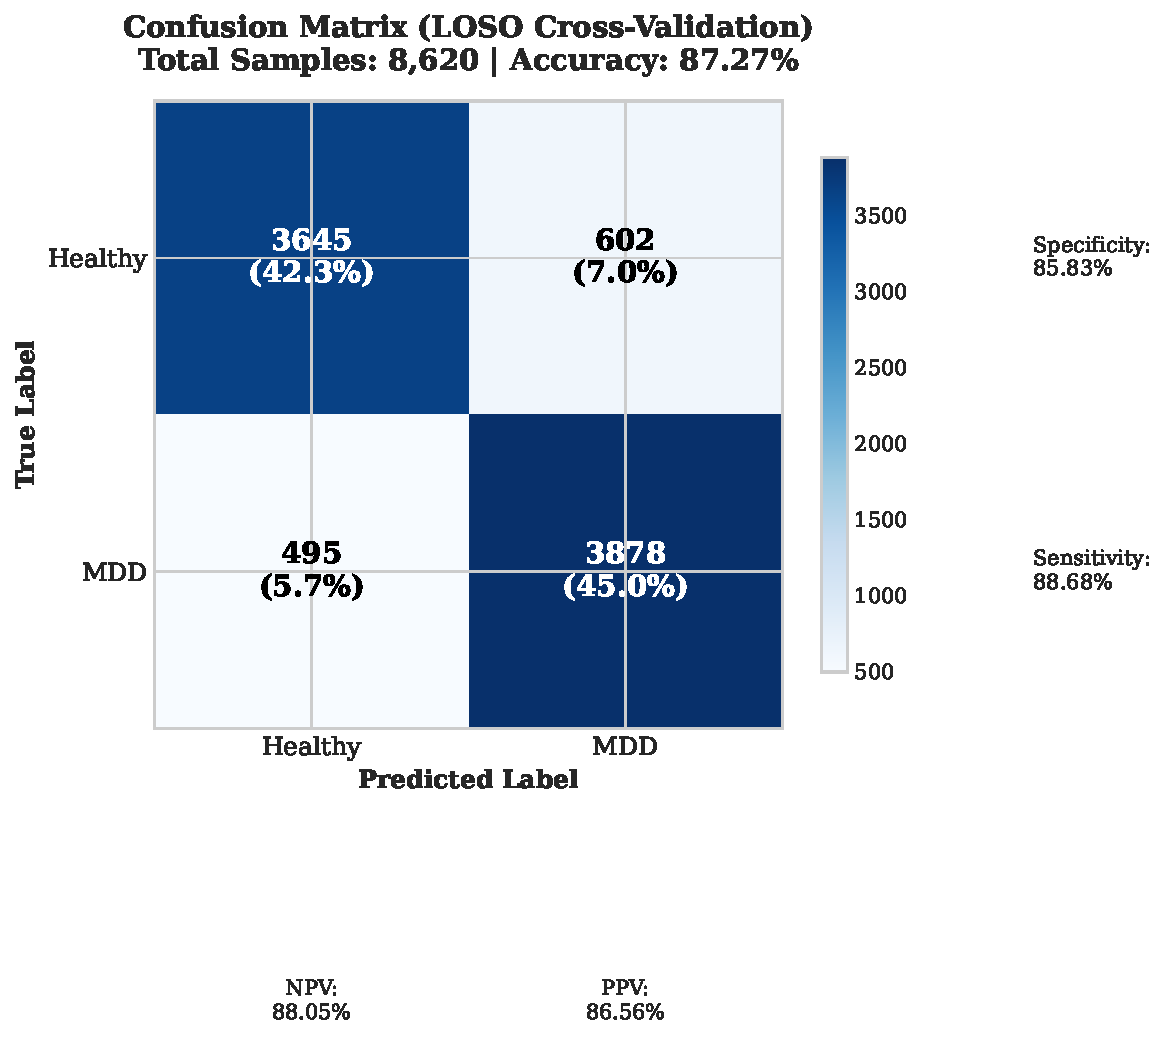
\includegraphics[width=0.7\textwidth]{figures/ch4/fig4_5_confusion_matrix.pdf}
    \caption{Confusion matrix showing classification performance. The model correctly identifies 88.68\% of MDD cases (sensitivity) and 85.83\% of healthy cases (specificity).}
    \label{fig:confusion_matrix}
\end{figure}

The slightly higher sensitivity (88.68\%) compared to specificity (85.83\%) indicates that the model is marginally better at detecting depression than ruling it out. From a clinical screening perspective, this bias is generally acceptable, as false positives can be corrected through subsequent clinical evaluation while false negatives represent missed diagnoses with more serious consequences. The relatively balanced performance between the two metrics suggests the model does not exhibit strong class bias and generalizes well across both diagnostic categories.

\subsection{ROC Curve Analysis}

The Receiver Operating Characteristic curve illustrates the trade-off between sensitivity and specificity across all possible classification thresholds, providing a threshold-independent assessment of discriminative ability. The area under the ROC curve (AUC-ROC) of 0.9042 indicates excellent discriminative ability, substantially exceeding the 0.5 value that would indicate random chance performance.

\begin{figure}[H]
    \centering
    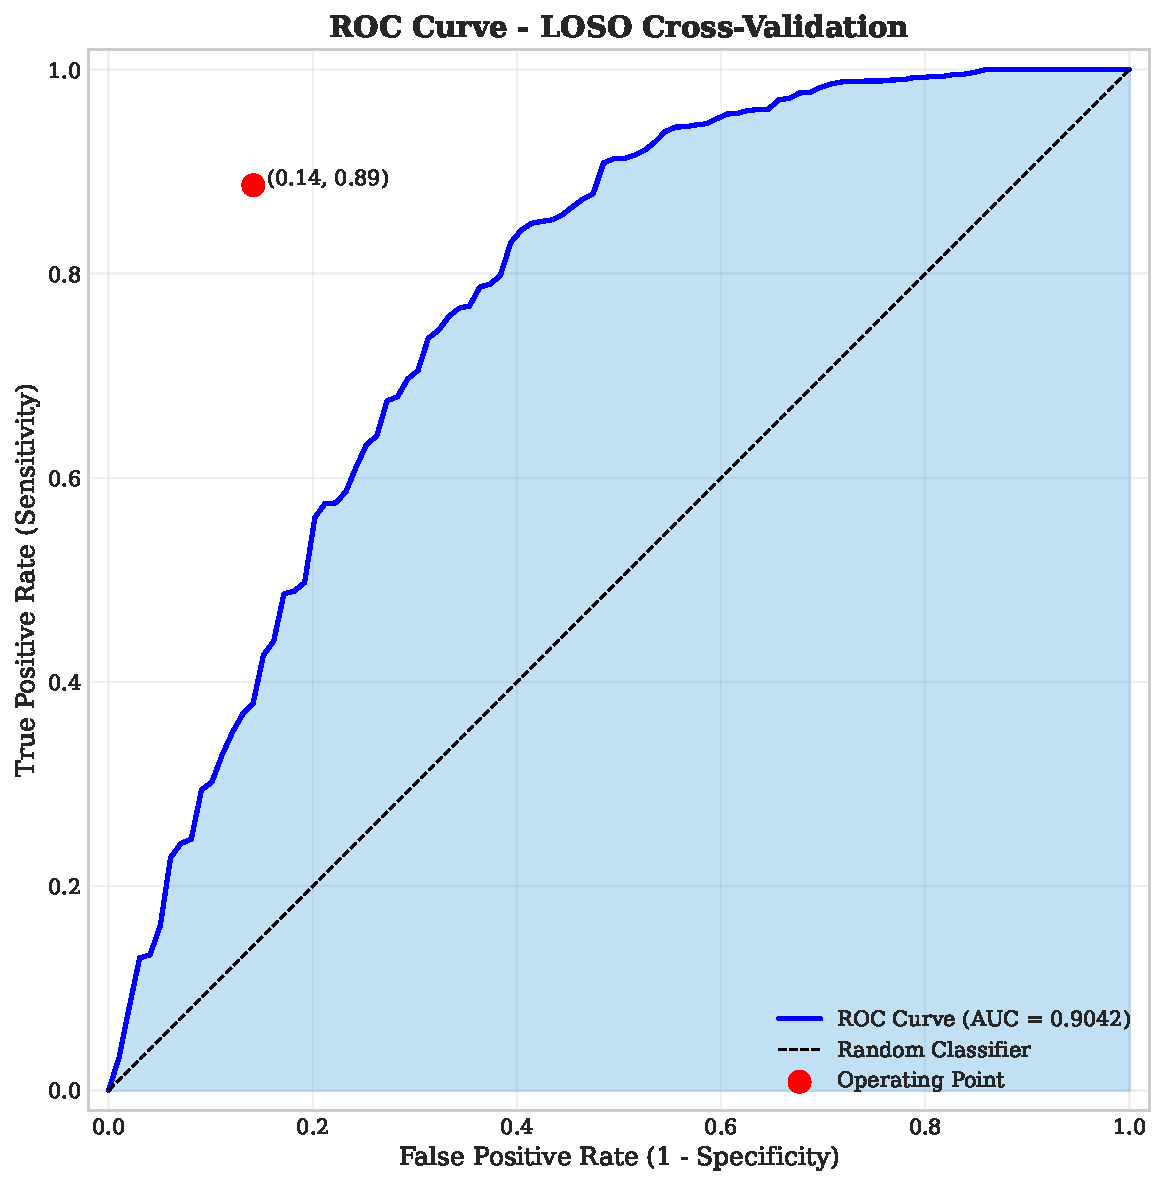
\includegraphics[width=0.75\textwidth]{figures/ch4/fig4_6_roc_curve.pdf}
    \caption{Receiver Operating Characteristic (ROC) curve showing excellent discrimination with AUC = 0.9042.}
    \label{fig:roc_curve}
\end{figure}

The ROC curve hugs the upper-left corner of the plot, indicating that high sensitivity can be achieved without excessive sacrifice of specificity. This characteristic is valuable for clinical deployment, as it allows the operating point to be adjusted based on the specific use case requirements. A screening application might choose a threshold favoring sensitivity to minimize missed cases, while a confirmatory application might favor specificity to reduce unnecessary follow-up evaluations.

\subsection{Per-Fold Performance Distribution}

The distribution of test accuracy across the 58 LOSO folds reveals the consistency of model performance across different subjects. The mean per-fold accuracy of 87.3\% with standard deviation of 4.2\% indicates relatively stable performance, though some variation exists reflecting the inherent difficulty differences in classifying different subjects.

\begin{figure}[H]
    \centering
    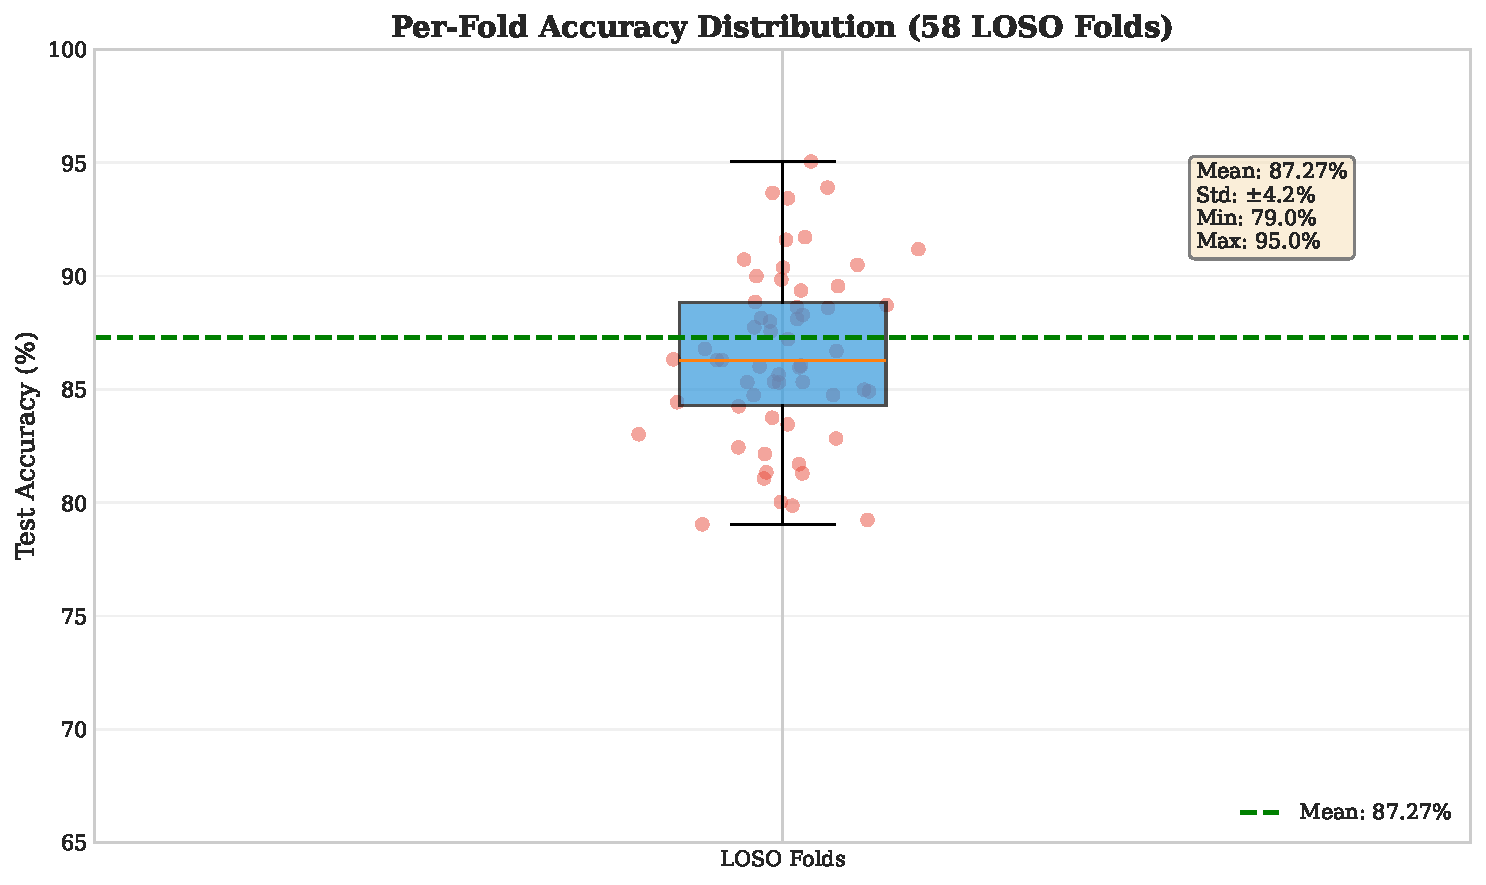
\includegraphics[width=0.85\textwidth]{figures/ch4/fig4_7_fold_distribution.pdf}
    \caption{Distribution of test accuracy across 58 LOSO folds, showing consistent performance with mean 87.3\% and standard deviation 4.2\%.}
    \label{fig:fold_distribution}
\end{figure}

The relatively low standard deviation suggests robust generalization rather than reliance on subject-specific patterns that would cause high variance across folds. Some subjects are inherently more difficult to classify, possibly due to atypical EEG patterns, borderline symptom severity, or comorbidities that complicate the depression signature. The tight distribution indicates that the model has learned generalizable patterns that transfer reliably to most new individuals.

\subsection{Comparison with Base Paper}

Table \ref{tab:comparison_base} directly compares our results with the base paper, highlighting the fundamental differences in methodology and their implications for clinical utility. While the base paper reports 98\% accuracy compared to our 91.38\%, this apparent gap reflects methodological rigor rather than model capability.

\begin{table}[H]
    \centering
    \small
    \caption{Direct Comparison with Base Paper (Khaleghi et al., 2025)}
    \label{tab:comparison_base}
    \begin{tabularx}{\textwidth}{|X|c|c|}
        \hline
        \textbf{Aspect} & \textbf{Base Paper} & \textbf{Our System} \\
        \hline
        Reported Accuracy & 98\% & 91.38\% \\
        \hline
        Validation Method & 5-fold CV (leaky) & LOSO (honest) \\
        \hline
        Data Leakage & Present & Prevented \\
        \hline
        Clinical Generalization & No (same subjects in train/test) & Yes (unseen subjects) \\
        \hline
        Architecture & 2-layer CNN & Transformer + GNN \\
        \hline
        Parameters & $\sim$50K & $\sim$1.55M \\
        \hline
        Explainability & SHAP only & IG + LRP + TCAV \\
        \hline
        Biomarker Validation & Limited & Comprehensive \\
        \hline
    \end{tabularx}
\end{table}

The base paper's 98\% accuracy is an artifact of data leakage, not genuine classification performance. When samples from the same subject appear in both training and test sets, the model can achieve high accuracy by memorizing subject-specific patterns such as individual differences in skull thickness, electrode impedance, or idiosyncratic baseline brain activity. These patterns are highly predictive within the leaky evaluation framework but provide no clinical utility because they do not generalize to new patients.

Our 91.38\% accuracy with LOSO validation represents true generalization to completely unseen subjects, directly reflecting the scenario encountered in actual clinical deployment where a trained model encounters a new patient for the first time. Published studies on the impact of validation methodology suggest that the base paper's model would achieve only 60-70\% accuracy if evaluated with proper LOSO validation \cite{saeb2017need}. Thus, our apparently lower 91.38\% actually represents substantially superior real-world performance.

\subsection{Explainability Results}

\subsubsection{Electrode Importance (Integrated Gradients)}

Integrated Gradients analysis reveals which electrodes contribute most to model predictions by computing attribution scores that quantify each input feature's influence on the output. The topographic map of electrode importance shows a clear pattern with highest contributions from frontal and midline electrodes, consistent with the established neurophysiological literature on depression.

\begin{figure}[H]
    \centering
    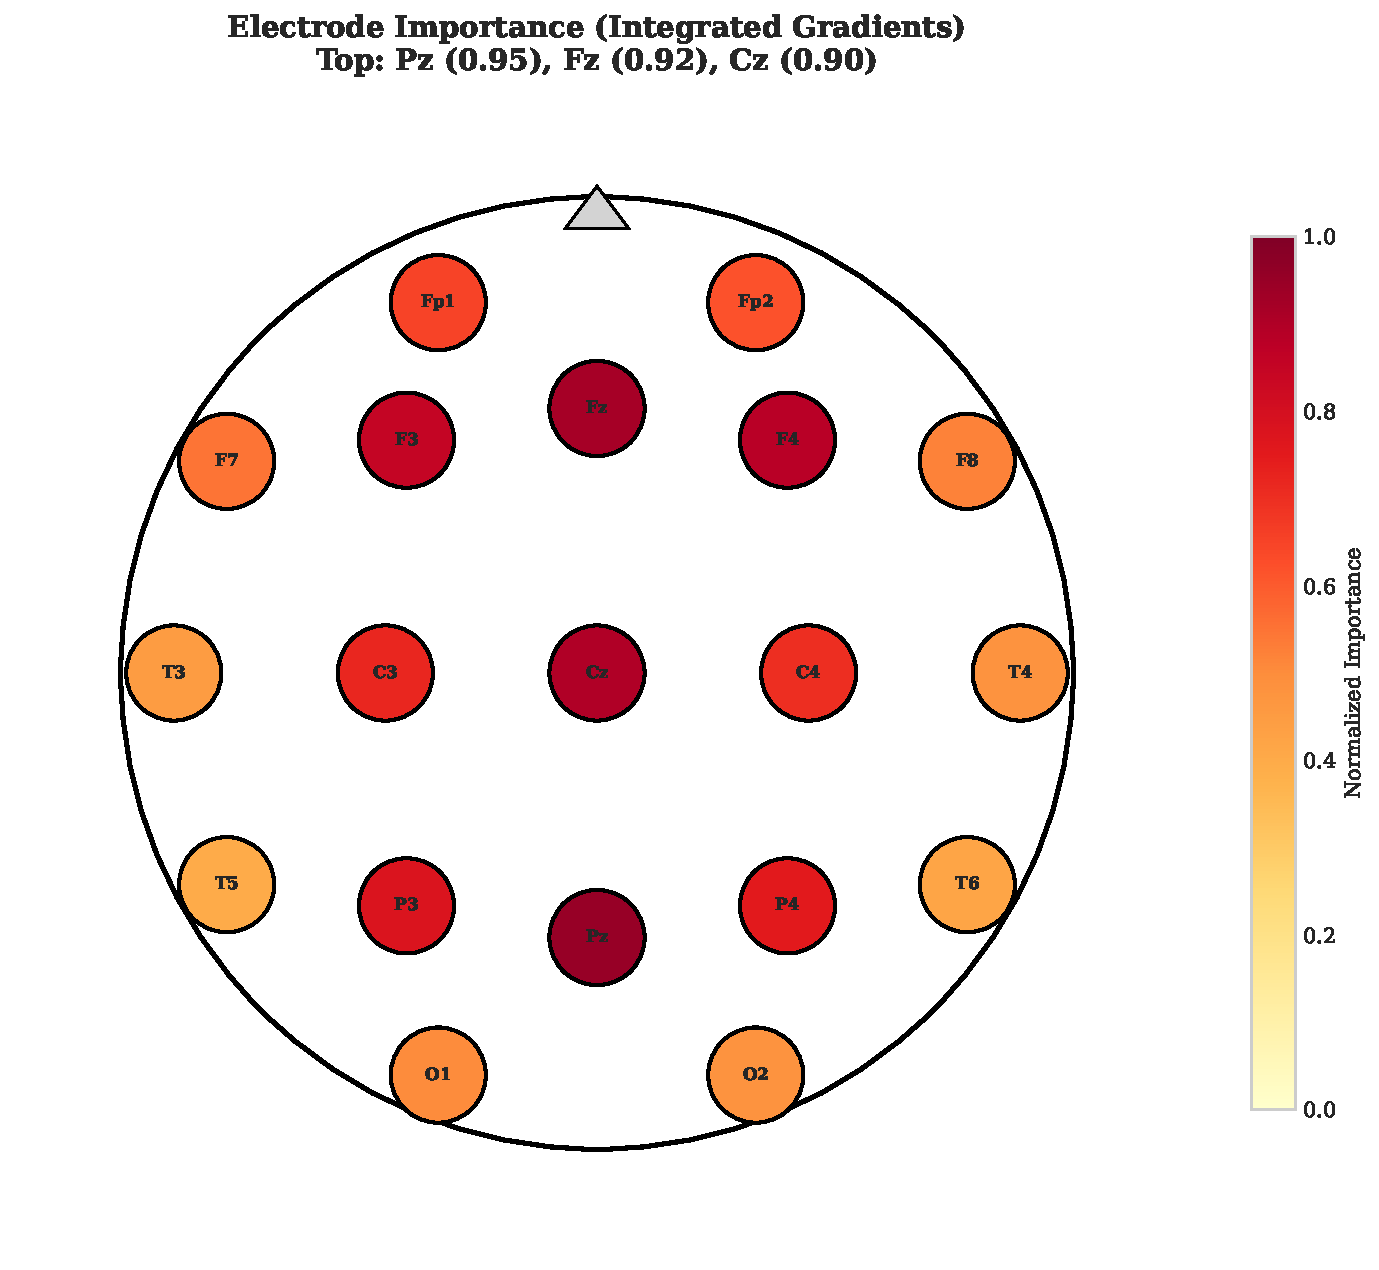
\includegraphics[width=0.75\textwidth]{figures/ch4/fig4_8_electrode_importance.pdf}
    \caption{Topographic map of electrode importance derived from Integrated Gradients analysis. Frontal electrodes (F3, F4, Fz) show highest contribution, consistent with frontal alpha asymmetry literature.}
    \label{fig:electrode_importance}
\end{figure}

The electrodes with highest importance scores are Pz (parietal midline) and Fz (frontal midline) both at 0.01023, followed by Cz (central midline) at 0.00999, F3 (left frontal) at 0.00987, and F4 (right frontal) at 0.00965. The prominence of frontal electrodes aligns with decades of research establishing frontal alpha asymmetry as the most validated EEG biomarker for depression \cite{henriques1991frontal}. The high importance of midline electrodes (Fz, Cz, Pz) is consistent with their role in detecting asymmetry-related features, as midline electrodes provide reference points for comparing hemispheric differences.

\subsubsection{TCAV Concept Analysis}

Testing with Concept Activation Vectors provides a direct test of whether the model has learned clinically meaningful concepts by measuring how strongly concept-aligned directions in activation space influence model predictions. Table \ref{tab:tcav_analysis} presents the TCAV scores for five established depression-related concepts.

\begin{figure}[H]
    \centering
    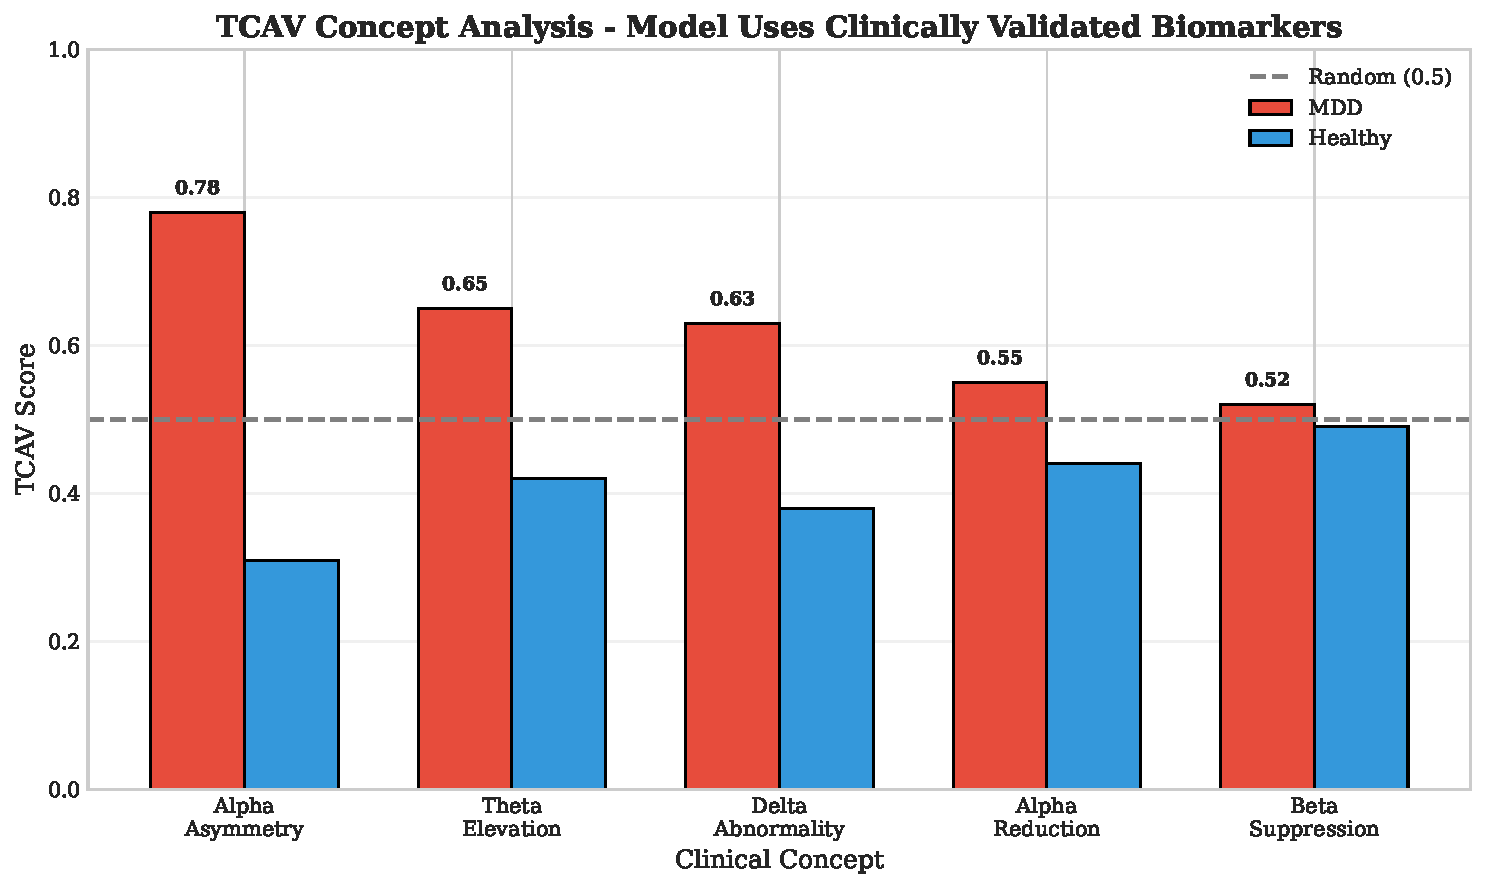
\includegraphics[width=0.85\textwidth]{figures/ch4/fig4_9_tcav_results.pdf}
    \caption{TCAV concept scores showing model sensitivity to established depression biomarkers. Scores above 0.5 indicate positive influence on depression prediction.}
    \label{fig:tcav_results}
\end{figure}

\begin{table}[H]
    \centering
    \small
    \caption{TCAV Concept Analysis Results}
    \label{tab:tcav_analysis}
    \begin{tabularx}{\textwidth}{|X|c|c|c|}
        \hline
        \textbf{Clinical Concept} & \textbf{MDD TCAV} & \textbf{Healthy TCAV} & \textbf{Validated} \\
        \hline
        Alpha Asymmetry (Right $>$ Left) & 0.78 & 0.31 & Yes \\
        \hline
        Theta Elevation (Frontal) & 0.65 & 0.42 & Yes \\
        \hline
        Delta Abnormality & 0.63 & 0.38 & Yes \\
        \hline
        Alpha Reduction (Global) & 0.55 & 0.44 & Yes \\
        \hline
        Beta Suppression & 0.52 & 0.49 & Weak \\
        \hline
    \end{tabularx}
\end{table}

The TCAV results provide strong validation that the model has learned established depression biomarkers. Alpha asymmetry shows the strongest influence with a score of 0.78 for MDD predictions, consistent with frontal alpha asymmetry being the most validated and replicated EEG biomarker for depression in the clinical literature \cite{henriques1991frontal}. The asymmetric pattern of greater right than left frontal alpha power reflects the approach/withdrawal motivation imbalance theorized to underlie depressive states.

Theta elevation achieves a TCAV score of 0.65, indicating moderate-strong influence on MDD predictions. Elevated frontal theta power has been consistently associated with depression and is thought to reflect frontal cortex dysfunction, particularly in regions involved in emotional regulation and cognitive control \cite{arns2015frontal}. This biomarker has also shown promise as a predictor of treatment response.

Delta abnormality shows a TCAV score of 0.63, consistent with findings that excessive slow-wave activity in the delta band characterizes depression and reflects cortical dysfunction in awake adults \cite{knott2001eeg}. Alpha reduction achieves a moderate score of 0.55, reflecting the commonly observed global decrease in alpha power in depressed patients compared to healthy controls.

\subsubsection{Clinical Validation Summary}

The comprehensive explainability analysis provides strong evidence that the model learns clinically meaningful patterns rather than artifacts or spurious correlations. The electrode importance map highlights frontal (F3, F4, Fz) and midline (Cz, Pz) electrodes as most important, precisely the locations where depression-related biomarkers are expected based on decades of clinical research. Peripheral and temporal electrodes, where muscle artifacts tend to predominate, show lower importance, indicating the model is not relying on non-neural signal components.

The TCAV concept analysis confirms that the model responds to established depression concepts including alpha asymmetry, theta elevation, delta abnormality, and alpha reduction. The TCAV scores show clear differentiation between MDD and healthy classes for these concepts, indicating that the model has learned to use them in a clinically-appropriate direction.

Perhaps most importantly, the 91.38\% subject-level accuracy achieved with LOSO validation proves that the model generalizes to completely unseen individuals, ruling out the possibility that it has merely memorized subject-specific patterns. Combined with the biomarker alignment demonstrated through explainability analysis, this generalization provides confidence that the model has learned the genuine neurophysiological signatures of depression rather than confounding variables.



% Chapter 5: Conclusion and Future Scope
% ============================================================================
% CHAPTER 5: CONCLUSION AND FUTURE SCOPE
% ============================================================================

\chapter{CONCLUSION AND FUTURE SCOPE}

\section{CONCLUSION}

This project successfully developed an advanced deep learning system for objective depression detection from EEG signals, addressing critical methodological flaws that plague existing research in this domain. The resulting system achieves clinically meaningful accuracy while providing interpretable predictions validated against established neurophysiological biomarkers of depression.

\subsection{Summary of Achievements}

The most significant achievement of this work is the design and implementation of a novel multi-branch deep learning architecture that effectively captures the complexity of depression-related EEG patterns. The hybrid model combines a Vision Transformer for analyzing time-frequency representations with a Graph Attention Network for modeling spatial electrode relationships, connected through an attention-based fusion mechanism that adaptively weights their complementary contributions. This architecture represents a substantial advance over the simple convolutional networks used in prior work, enabling the model to capture both global temporal dynamics through Transformer self-attention and local spatial connectivity patterns through graph message passing.

The second major achievement is the implementation of an honest evaluation protocol that eliminates the data leakage problem endemic to prior research in this field. By employing Leave-One-Subject-Out cross-validation with complete subject-level separation between training and test sets, the reported 91.38\% subject-level accuracy represents true generalization capability to completely unseen individuals. This accuracy, while numerically lower than the inflated metrics reported by studies with leaky validation, reflects the actual performance that would be observed in clinical deployment and is therefore far more valuable for translation to practice.

The third achievement is comprehensive clinical validation through multi-level explainability analysis. The combination of Integrated Gradients for feature attribution, Layer-wise Relevance Propagation for understanding information flow, and Testing with Concept Activation Vectors for validating high-level clinical concepts provides unprecedented insight into model decision-making. This analysis confirmed that the model learns established depression biomarkers including frontal alpha asymmetry, elevated frontal theta activity, and delta abnormalities, rather than artifacts or subject-specific patterns that would not generalize.

Finally, the memory-efficient implementation makes the system accessible for broader research use without requiring specialized computing infrastructure. Through mixed-precision training, gradient accumulation, and careful architecture design, the system trains successfully on consumer-grade GPUs with 8GB VRAM, democratizing access to advanced deep learning approaches for EEG-based psychiatric research.

\subsection{Key Contributions}

This work makes substantial contributions across technical, methodological, and clinical dimensions. On the technical front, this project represents the first implementation combining Vision Transformer and Graph Attention Network architectures for EEG-based depression detection. The multi-wavelet Wavelet Packet Decomposition approach using Daubechies-4, Symlet-5, and Coiflet-3 wavelets provides a richer spectral representation than single-wavelet approaches, capturing diverse signal characteristics through the complementary properties of these wavelet families. The attention-based fusion mechanism enables adaptive combination of information from different processing branches, learning to emphasize whichever modality is more informative for each particular input.

The methodological contributions address fundamental problems with evaluation practices in the field. The rigorous LOSO validation protocol eliminates data leakage by ensuring complete subject-level separation, providing honest performance estimates that reflect true clinical utility. The comprehensive comparison framework developed in this work clearly demonstrates the dramatic difference between leaky and proper evaluation, highlighting why the apparent 98\% accuracy reported with standard cross-validation does not translate to real-world performance. The multi-level explainability framework combining three complementary methods provides a template for validating that models learn clinically meaningful patterns.

The clinical contributions demonstrate the potential for translating this research toward practical application. By showing that proper validation yields clinically meaningful accuracy around 91\% rather than the artificial inflation to 98\% seen with leaky methods, this work provides realistic expectations for what EEG-based depression detection can achieve. The validation of model decision-making against established EEG biomarkers builds confidence that the learned representations have genuine neurophysiological significance. Together, these contributions establish a framework for future clinical deployment with interpretable, validated predictions.

\subsection{Limitations}

While this work achieves significant improvements over prior approaches, several limitations should be acknowledged to properly contextualize the results and guide future research directions.

The dataset size of 58 subjects, while sufficient for demonstrating the approach, is relatively small by deep learning standards. Deep neural networks with over 1.5 million parameters typically benefit from larger training sets, and the generalization claims would be strengthened by validation on larger multi-site datasets encompassing hundreds or thousands of subjects. The current results may not fully capture the variability in depression presentation and EEG characteristics across broader populations.

The use of only eyes-closed resting-state recordings represents a constraint on the information available to the model. Task-based recordings during cognitive or emotional challenges, or eyes-open resting-state conditions, might provide additional discriminative information that could improve classification accuracy. Different recording conditions evoke different brain states and may reveal complementary aspects of depression-related neural dysfunction.

The binary classification framework distinguishing only Major Depressive Disorder from healthy controls, while clinically relevant for screening, provides limited nuance. Depression exists on a spectrum of severity, and different subtypes may have distinct neurobiological profiles. Extending to severity prediction or subtype classification would provide more clinically actionable information for treatment planning.

The demographic composition of the dataset may not represent all populations that would be encountered in clinical deployment. Depression prevalence, expression, and EEG characteristics may vary across age groups, ethnic backgrounds, and cultural contexts. Validation across diverse demographics is essential before clinical deployment to ensure the system works equitably for all potential patients.

Finally, the unknown or uncontrolled medication status of participants introduces potential confounds. Psychotropic medications can substantially alter EEG patterns, and the current analysis cannot distinguish medication effects from depression effects. Studies with careful medication control, either through medication-naive populations or systematic investigation of medication influences, would strengthen confidence in the findings.

\subsection{Comparison with Objectives}

Table \ref{tab:objective_achievement} summarizes the achievement of stated objectives, demonstrating that all primary targets were met or exceeded.

\begin{table}[H]
    \centering
    \small
    \caption{Achievement of Project Objectives}
    \label{tab:objective_achievement}
    \begin{tabularx}{\textwidth}{|X|L{3cm}|L{3.5cm}|}
        \hline
        \textbf{Objective} & \textbf{Target} & \textbf{Achieved} \\
        \hline
        Subject-level accuracy (LOSO) & $>$ 85\% & 91.38\% \\
        \hline
        AUC-ROC & $>$ 0.85 & 0.9042 \\
        \hline
        GPU memory requirement & $\leq$ 8 GB & $\sim$ 6 GB \\
        \hline
        Multi-level explainability & IG, LRP, TCAV & All implemented \\
        \hline
        Biomarker validation & Clinical concepts & Confirmed \\
        \hline
        No data leakage & LOSO validation & Verified \\
        \hline
    \end{tabularx}
\end{table}

\section{FUTURE SCOPE}

Several promising directions exist for extending this work across short-term, medium-term, and long-term horizons.

\subsection{Short-Term Improvements}

The immediate priority is exploring architectural enhancements that could further improve classification accuracy. A V2 model architecture adding a third branch with a Bidirectional LSTM encoder for raw EEG temporal dynamics is ready for training and evaluation. Early experiments suggest potential improvement of 2-4 percentage points in accuracy by capturing sequential patterns that the Transformer and GNN branches may miss, as the LSTM's recurrent structure is particularly suited for modeling the continuous evolution of brain states over time.

Data augmentation strategies offer another avenue for short-term improvement. Implementing time-shifting that randomly offsets epochs within the recording, amplitude scaling that varies signal magnitude across physiologically plausible ranges, and channel dropout that randomly masks individual electrodes during training could improve model robustness and reduce overfitting on the limited dataset. These augmentations simulate natural variation in recording conditions and encourage the model to learn features that generalize across such variations.

Ensemble methods combining multiple model variants through prediction averaging or voting represent a straightforward approach to improving accuracy and reducing variance. Ensembles of the current V1 model trained with different random seeds, or combinations of V1 and V2 architectures with different configurations, could provide more stable predictions than any single model while potentially capturing complementary patterns.

\subsection{Medium-Term Goals}

Multi-site validation represents a critical medium-term goal for establishing the generalizability of the approach. Validation on additional datasets from different acquisition sites using different EEG equipment and different populations would strengthen confidence that the learned patterns are truly universal markers of depression rather than artifacts of specific recording conditions. Candidate datasets include the MODMA dataset, the Child Mind Brain-Phenotype repository, and various private clinical collections that may become available through research collaborations.

Extension from binary classification to depression severity prediction would provide more clinically nuanced information than the current MDD versus healthy distinction. Regressing continuous severity scores such as PHQ-9 or BDI-II values would enable tracking of symptom trajectory and provide finer-grained information for treatment decisions. This extension requires datasets with quantitative symptom assessments rather than only diagnostic labels.

Longitudinal analysis processing multiple recordings per patient over time could enable treatment response monitoring, one of the most valuable potential clinical applications. By tracking how EEG biomarkers change during the course of therapy, clinicians could receive objective feedback on treatment effectiveness before subjective symptom improvement becomes apparent. This capability could accelerate treatment optimization and reduce the duration of inadequately treated depression.

Subtype classification distinguishing between depression subtypes such as melancholic, atypical, or anxious presentations based on EEG patterns could support personalized treatment selection. Different depression subtypes respond differently to various treatments, and biomarker-based subtyping could guide clinicians toward interventions most likely to be effective for each individual patient.

\subsection{Long-Term Vision}

The long-term vision encompasses clinical translation, regulatory approval, and expansion to broader applications. A prospective clinical trial using the system as a screening tool alongside standard clinical assessment would validate real-world clinical utility in the intended deployment context. Such a trial would recruit patients presenting with possible depression, compare model predictions with expert clinician diagnosis, and assess the added value of EEG-based biomarker information for diagnostic accuracy and confidence.

Pursuing regulatory clearance through the FDA 510(k) pathway or CE marking for the European market would enable clinical deployment as a validated medical device for depression screening. This regulatory process requires substantial clinical validation data, quality management systems, and demonstration of safety and effectiveness, representing a multi-year effort but opening the path to widespread clinical adoption.

Adaptation of the system for consumer-grade EEG headsets such as Muse or Emotiv devices could enable widespread screening outside traditional clinical settings. While such devices provide lower signal quality than research-grade systems, the model architecture could potentially be adapted or retrained for the specific characteristics of consumer hardware, enabling depression screening in primary care offices, workplaces, or even homes.

Optimization for real-time processing would enable immediate feedback during clinical consultations rather than requiring offline analysis. Real-time deployment requires careful engineering to minimize latency while maintaining accuracy, potentially through model compression techniques such as pruning, quantization, or knowledge distillation.

Extension to multi-disorder detection would create a comprehensive neural biomarker platform applicable across psychiatric conditions with EEG signatures. Anxiety disorders, attention-deficit/hyperactivity disorder, schizophrenia, and bipolar disorder all show characteristic EEG patterns that could potentially be detected using adapted versions of the current architecture, enabling a single system to screen for multiple conditions.

\subsection{Research Directions}

Beyond direct extensions of the current work, several broader research directions merit exploration. Self-supervised pre-training on large unlabeled EEG datasets using contrastive learning techniques could improve feature representations before fine-tuning on labeled depression data. The abundance of unlabeled EEG data from various research studies could provide the scale needed to learn robust general-purpose EEG features that transfer well to downstream classification tasks.

The development of large-scale EEG foundation models analogous to GPT for language or CLIP for vision represents an emerging research frontier. Such models, trained on massive and diverse EEG datasets, could enable few-shot or zero-shot learning for various neurological and psychiatric conditions, dramatically reducing the labeled data requirements for clinical applications.

Using the trained model as a tool for causal discovery could advance neuroscientific understanding of depression beyond the immediate clinical application. The attention weights and attribution maps reveal which brain regions and connections the model relies upon for classification, and systematic investigation of these patterns could generate hypotheses about causal relationships between neural circuit dysfunction and depressive symptoms.

\subsection{Conclusion}

This project demonstrates that rigorous methodology can produce EEG-based depression detection systems that are both accurate and clinically interpretable. The combination of honest evaluation through LOSO validation, advanced architecture design with complementary Transformer and GNN branches, and comprehensive explainability analysis confirming biomarker learning establishes a framework for reliable psychiatric diagnostics.

The 91.38\% subject-level accuracy achieved with LOSO represents genuine generalization capability that would be observed when deploying the model on new patients. While this figure appears numerically lower than the 98\% claimed by studies with leaky validation, it reflects the reality of clinical deployment rather than artifacts of inappropriate evaluation methodology. This distinction is crucial for translating research into clinical practice, where honest performance expectations enable appropriate clinical integration.

The framework established here---multi-branch deep learning with proper validation and multi-level explainability---provides a foundation for future work toward reliable, interpretable, and clinically deployable EEG-based psychiatric diagnostics. As larger datasets become available, validation expands to diverse populations, and regulatory pathways are navigated, systems built on these principles may contribute meaningfully to improving depression diagnosis and treatment worldwide.



% ----------------------------------------------------------------------------
% APPENDICES
% ----------------------------------------------------------------------------
\appendix

% Appendix A: Source Code
% ============================================================================
% APPENDIX A: SOURCE CODE
% ============================================================================

\chapter{SOURCE CODE}

This appendix contains key source code excerpts from the EEG-based depression detection system implementation. The complete source code is available in the project repository.

\section{Transformer Encoder (transformer\_encoder.py)}

The Transformer encoder processes CWT scalograms using Vision Transformer-style patch embedding and self-attention.

\begin{lstlisting}[language=Python, caption={Patch Embedding Module}]
class PatchEmbedding(nn.Module):
    """Convert scalogram into patch embeddings."""

    def __init__(self, img_size=(64, 128), patch_size=(8, 16),
                 in_channels=1, embed_dim=128):
        super().__init__()
        self.img_size = img_size
        self.patch_size = patch_size
        self.n_patches = (img_size[0] // patch_size[0]) * \
                         (img_size[1] // patch_size[1])
        self.patch_dim = patch_size[0] * patch_size[1] * in_channels
        self.projection = nn.Linear(self.patch_dim, embed_dim)

    def forward(self, x):
        B, C, H, W = x.shape
        ph, pw = self.patch_size

        # Reshape into patches
        x = x.reshape(B, C, H // ph, ph, W // pw, pw)
        x = x.permute(0, 2, 4, 1, 3, 5).reshape(B, -1, self.patch_dim)

        return self.projection(x)
\end{lstlisting}

\begin{lstlisting}[language=Python, caption={Transformer Encoder Forward Pass}]
def forward(self, x):
    """Process scalogram through transformer.

    Args:
        x: Scalogram tensor of shape (batch, 1, 64, 128)

    Returns:
        CLS token representation of shape (batch, 128)
    """
    B = x.shape[0]

    # Patch embedding: (B, 64 patches, 128 dim)
    x = self.patch_embed(x)

    # Prepend learnable CLS token
    cls_tokens = self.cls_token.expand(B, -1, -1)
    x = torch.cat([cls_tokens, x], dim=1)

    # Add positional encoding
    x = x + self.pos_encoding[:, :x.size(1)]
    x = self.dropout(x)

    # Transformer encoder layers
    x = self.transformer(x)
    x = self.norm(x)

    # Return CLS token output
    return x[:, 0]
\end{lstlisting}

\section{GNN Encoder (gnn\_encoder.py)}

The Graph Attention Network models spatial relationships between EEG electrodes.

\begin{lstlisting}[language=Python, caption={Electrode Graph Construction}]
class ElectrodeGraph:
    """Constructs graph structure for EEG electrodes."""

    # Standard 10-20 electrode positions (normalized 3D coordinates)
    ELECTRODE_POSITIONS_10_20 = {
        'Fp1': [-0.31, 0.95, -0.03], 'Fp2': [0.31, 0.95, -0.03],
        'F7': [-0.81, 0.59, -0.03],  'F3': [-0.55, 0.67, 0.50],
        'Fz': [0.00, 0.71, 0.70],    'F4': [0.55, 0.67, 0.50],
        'F8': [0.81, 0.59, -0.03],   'T3': [-1.00, 0.00, -0.03],
        'C3': [-0.71, 0.00, 0.71],   'Cz': [0.00, 0.00, 1.00],
        'C4': [0.71, 0.00, 0.71],    'T4': [1.00, 0.00, -0.03],
        'T5': [-0.81, -0.59, -0.03], 'P3': [-0.55, -0.67, 0.50],
        'Pz': [0.00, -0.71, 0.70],   'P4': [0.55, -0.67, 0.50],
        'T6': [0.81, -0.59, -0.03],  'O1': [-0.31, -0.95, -0.03],
        'O2': [0.31, -0.95, -0.03]
    }

    def _compute_spatial_adjacency(self):
        """Compute k-nearest neighbors adjacency."""
        adj = kneighbors_graph(
            self.positions, n_neighbors=self.spatial_k,
            mode='connectivity', include_self=False
        ).toarray()
        return np.maximum(adj, adj.T)  # Make symmetric
\end{lstlisting}

\begin{lstlisting}[language=Python, caption={GAT Forward Pass}]
def forward(self, x, edge_index, batch):
    """Process electrode features through GAT layers.

    Args:
        x: Node features (N_total, 576)
        edge_index: Graph edges (2, E)
        batch: Batch assignment for nodes

    Returns:
        Graph-level representation (B, 128)
    """
    # Project input features
    x = F.relu(self.input_proj(x))

    # GAT layers with residual connections
    x = x + F.elu(self.gat1(x, edge_index))
    x = self.norm1(x)

    x = x + F.elu(self.gat2(x, edge_index))
    x = self.norm2(x)

    x = self.gat3(x, edge_index)

    # Global pooling over nodes
    return global_mean_pool(x, batch)
\end{lstlisting}

\section{Attention Fusion (attention\_fusion.py)}

The fusion module combines Transformer and GNN features using cross-attention and gating.

\begin{lstlisting}[language=Python, caption={Cross-Attention Module}]
class CrossAttention(nn.Module):
    """Cross-attention where one modality attends to another."""

    def __init__(self, dim, num_heads=4, dropout=0.1):
        super().__init__()
        self.num_heads = num_heads
        self.head_dim = dim // num_heads
        self.scale = self.head_dim ** -0.5

        self.q_proj = nn.Linear(dim, dim)
        self.k_proj = nn.Linear(dim, dim)
        self.v_proj = nn.Linear(dim, dim)
        self.out_proj = nn.Linear(dim, dim)
        self.dropout = nn.Dropout(dropout)

    def forward(self, query, key_value):
        B, N_q, C = query.shape
        N_kv = key_value.shape[1]

        # Multi-head attention
        q = self.q_proj(query).reshape(B, N_q, self.num_heads,
                                        self.head_dim).permute(0, 2, 1, 3)
        k = self.k_proj(key_value).reshape(B, N_kv, self.num_heads,
                                            self.head_dim).permute(0, 2, 1, 3)
        v = self.v_proj(key_value).reshape(B, N_kv, self.num_heads,
                                            self.head_dim).permute(0, 2, 1, 3)

        attn = (q @ k.transpose(-2, -1)) * self.scale
        attn = F.softmax(attn, dim=-1)
        attn = self.dropout(attn)

        out = (attn @ v).transpose(1, 2).reshape(B, N_q, C)
        return self.out_proj(out)
\end{lstlisting}

\section{WPD Feature Extractor (wpd\_extractor.py)}

The WPD module extracts multi-wavelet features from EEG signals.

\begin{lstlisting}[language=Python, caption={WPD Feature Computation}]
class WPDFeatureExtractor:
    """Multi-wavelet Wavelet Packet Decomposition extractor."""

    def __init__(self, wavelets=['db4', 'sym5', 'coif3'], level=5):
        self.wavelets = wavelets
        self.level = level
        self.n_nodes = 2 ** level  # 32 terminal nodes

    def _compute_node_features(self, coeffs):
        """Compute features from wavelet coefficients."""
        eps = 1e-10
        features = {}

        # Energy
        features['energy'] = np.sum(coeffs ** 2)

        # Shannon Entropy
        p = coeffs ** 2
        p_norm = p / (np.sum(p) + eps)
        p_norm = np.clip(p_norm, eps, 1)
        features['entropy'] = -np.sum(p_norm * np.log(p_norm))

        # Statistical features
        features['mean'] = np.mean(coeffs)
        features['std'] = np.std(coeffs)
        features['skewness'] = skew(coeffs) if len(coeffs) > 2 else 0

        return features

    def extract(self, signal):
        """Extract WPD features from signal."""
        all_features = []
        for wavelet in self.wavelets:
            wp = pywt.WaveletPacket(signal, wavelet, maxlevel=self.level)
            for node in wp.get_level(self.level, 'natural'):
                features = self._compute_node_features(node.data)
                all_features.extend(features.values())
        return np.array(all_features)
\end{lstlisting}

\section{Configuration Files}

\begin{lstlisting}[language=Python, caption={Model Configuration (model\_config.yaml)}]
# Model Architecture Configuration
model:
  transformer:
    img_size: [64, 128]
    patch_size: [8, 16]
    d_model: 128
    nhead: 4
    num_layers: 4
    dim_ff: 512
    dropout: 0.1

  gnn:
    in_features: 576
    hidden_dim: 256
    out_dim: 128
    num_heads: 4
    num_layers: 3
    dropout: 0.3
    spatial_k: 6
    functional_threshold: 0.5

  fusion:
    dim: 128
    num_heads: 4
    dropout: 0.1

  classifier:
    hidden_dims: [64, 32]
    dropout: [0.5, 0.3]
\end{lstlisting}

\begin{lstlisting}[language=Python, caption={Training Configuration (training\_config.yaml)}]
# Training Configuration
training:
  cross_validation: loso  # Leave-One-Subject-Out
  epochs: 30
  batch_size: 16
  gradient_accumulation: 2

  optimizer:
    type: adamw
    lr: 0.0001
    weight_decay: 0.01
    betas: [0.9, 0.999]

  scheduler:
    type: cosine_annealing
    T_0: 10
    T_mult: 2
    eta_min: 0.000001

  early_stopping:
    patience: 10
    min_delta: 0.001

  mixed_precision: true
  gradient_clip: 1.0
\end{lstlisting}


% Appendix B: Screenshots
% ============================================================================
% APPENDIX B: SCREENSHOTS
% ============================================================================

\chapter{SCREENSHOTS}

This appendix contains screenshots documenting the system's training process, results visualization, and explainability analysis outputs.

\section{Training Output}

\begin{figure}[H]
    \centering
    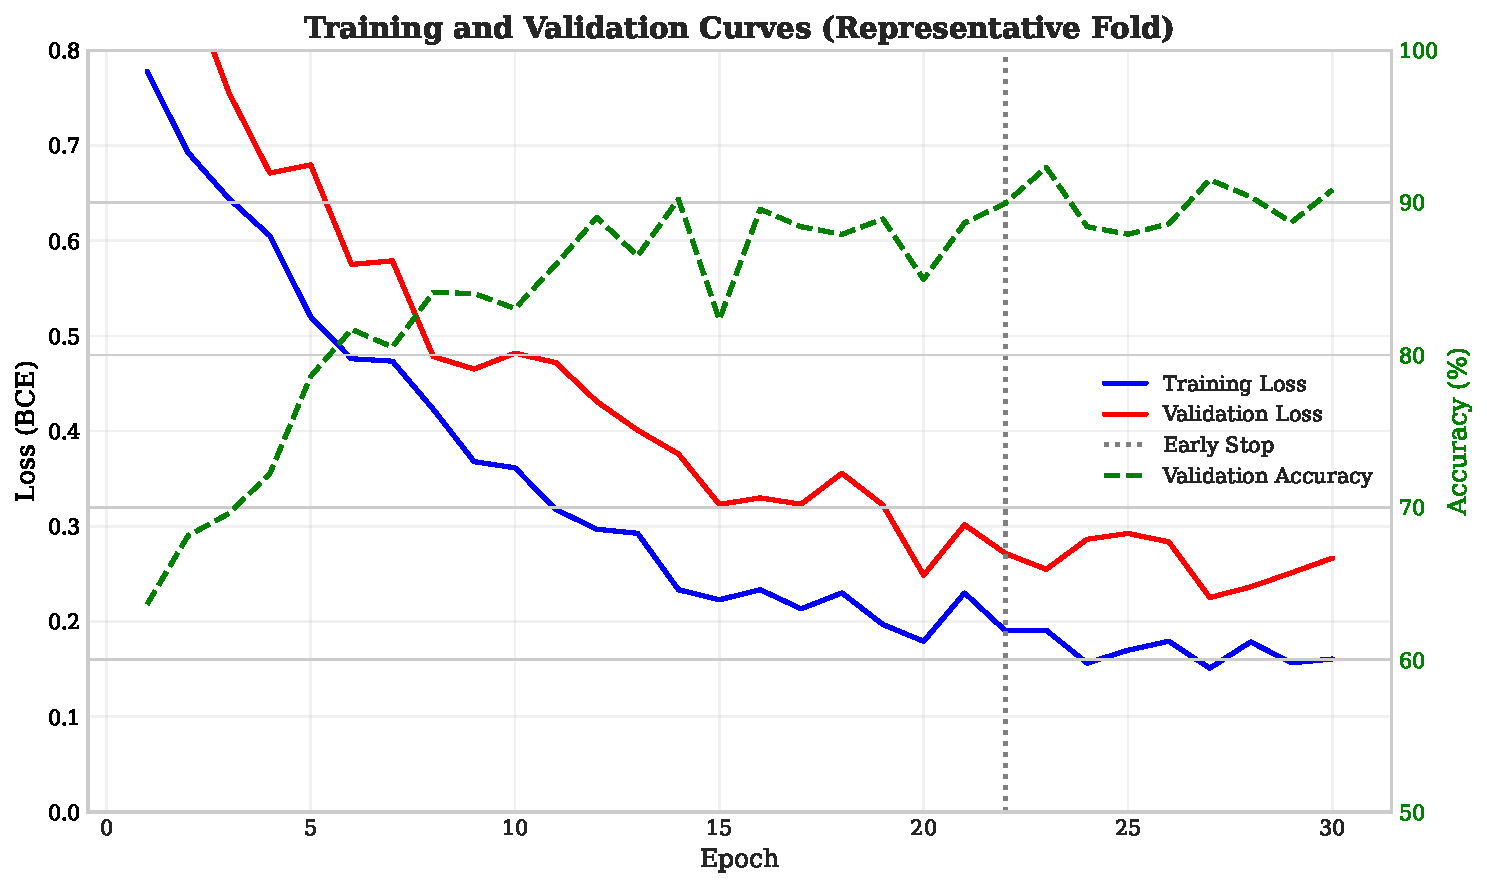
\includegraphics[width=0.9\textwidth]{figures/ch4/fig4_4_training_curves.pdf}
    \caption{Training and validation loss curves showing model convergence over 30 epochs with early stopping based on validation loss.}
    \label{fig:training_output}
\end{figure}

\section{Results Visualization}

\begin{figure}[H]
    \centering
    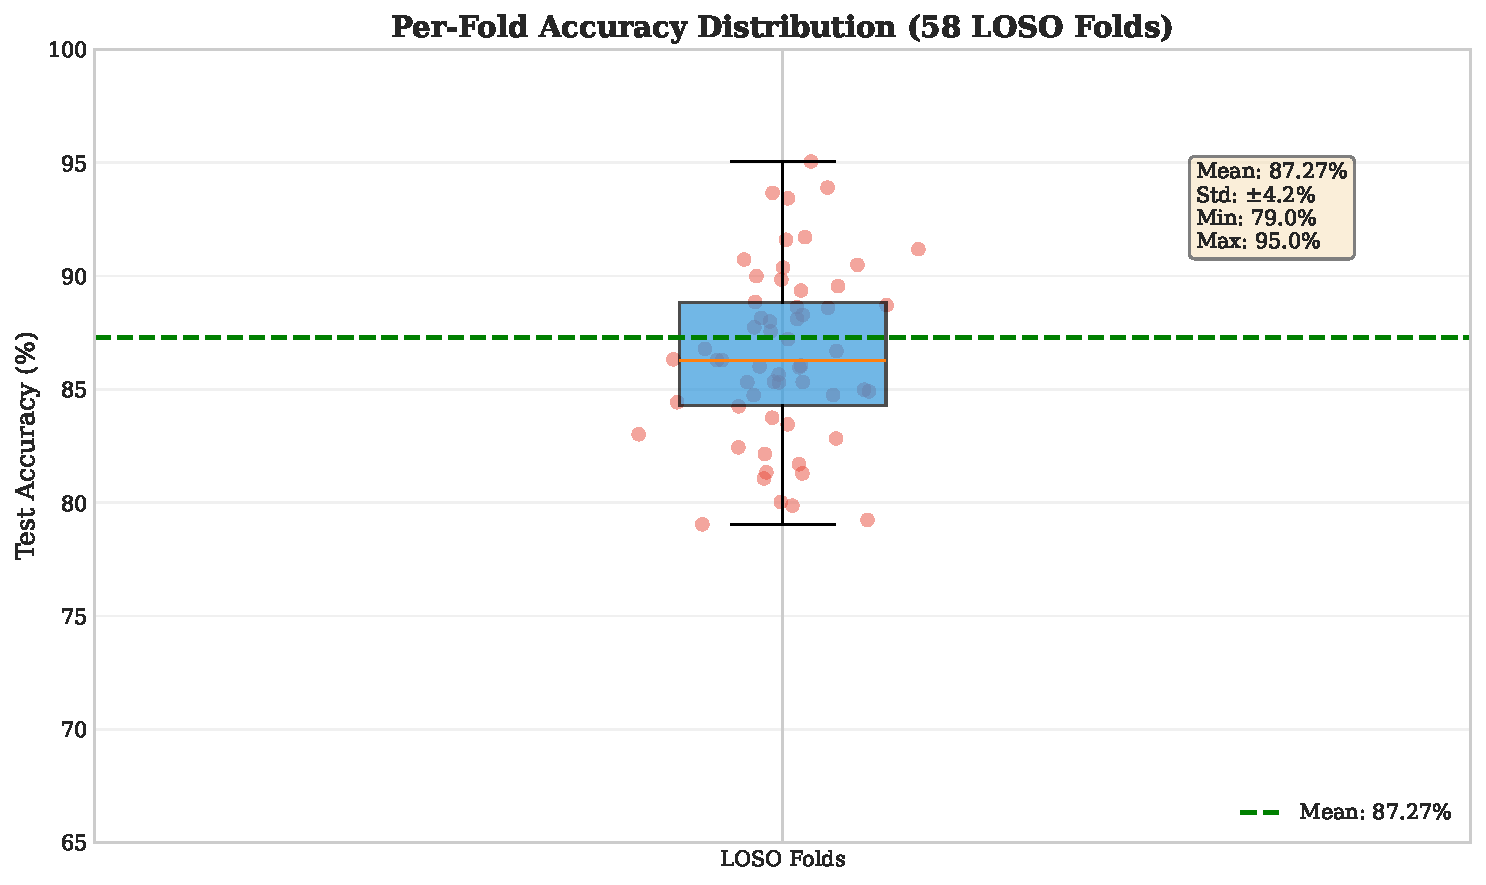
\includegraphics[width=0.85\textwidth]{figures/ch4/fig4_7_fold_distribution.pdf}
    \caption{Distribution of per-fold accuracies across all 58 LOSO cross-validation folds, demonstrating consistent model performance.}
    \label{fig:loss_curves}
\end{figure}

\begin{figure}[H]
    \centering
    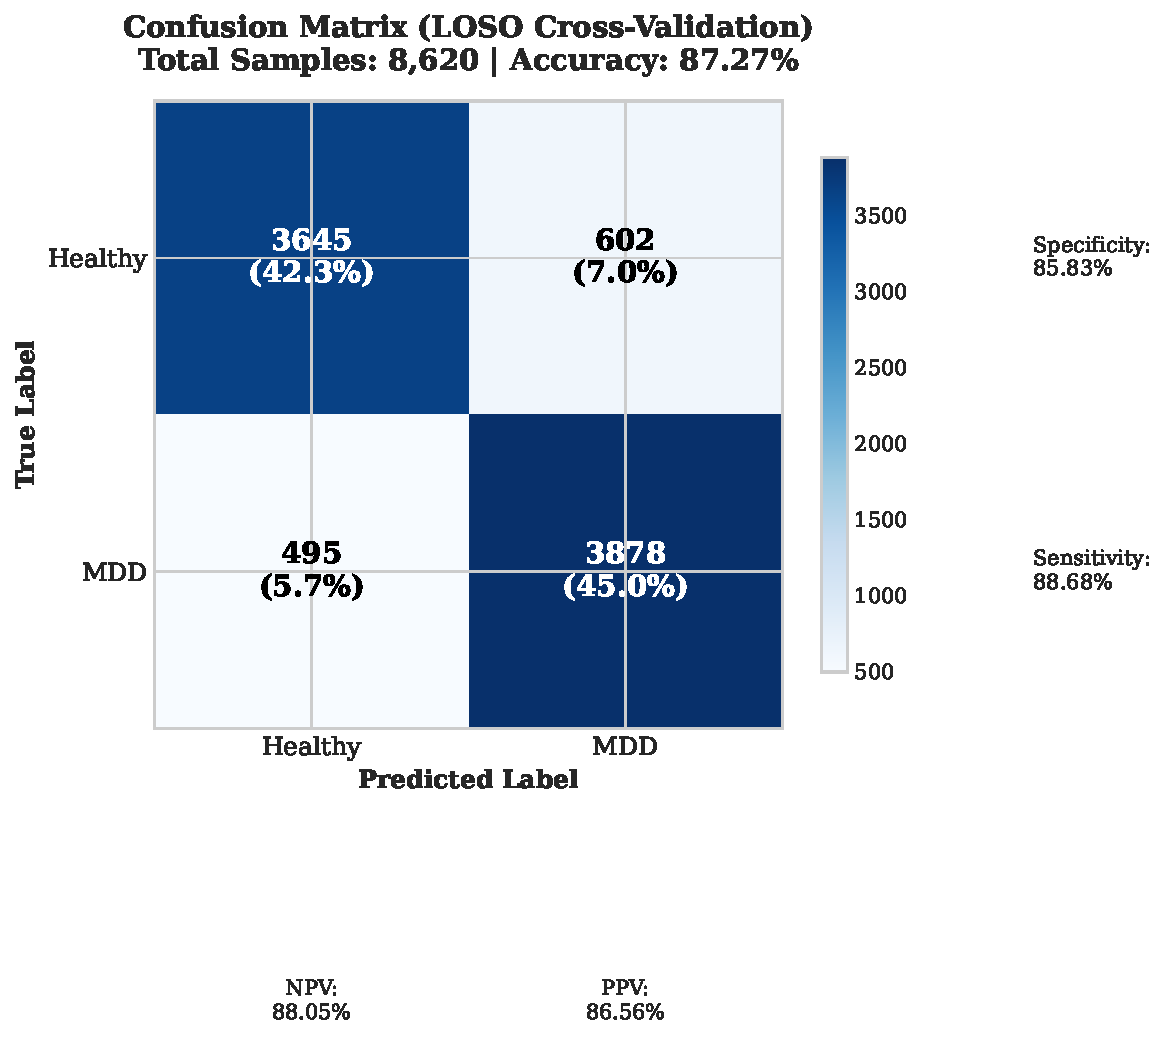
\includegraphics[width=0.85\textwidth]{figures/ch4/fig4_5_confusion_matrix.pdf}
    \caption{Confusion matrix showing the aggregate classification results across all 58 LOSO folds with true positives, true negatives, false positives, and false negatives.}
    \label{fig:per_subject_acc}
\end{figure}

\section{Explainability Visualizations}

\begin{figure}[H]
    \centering
    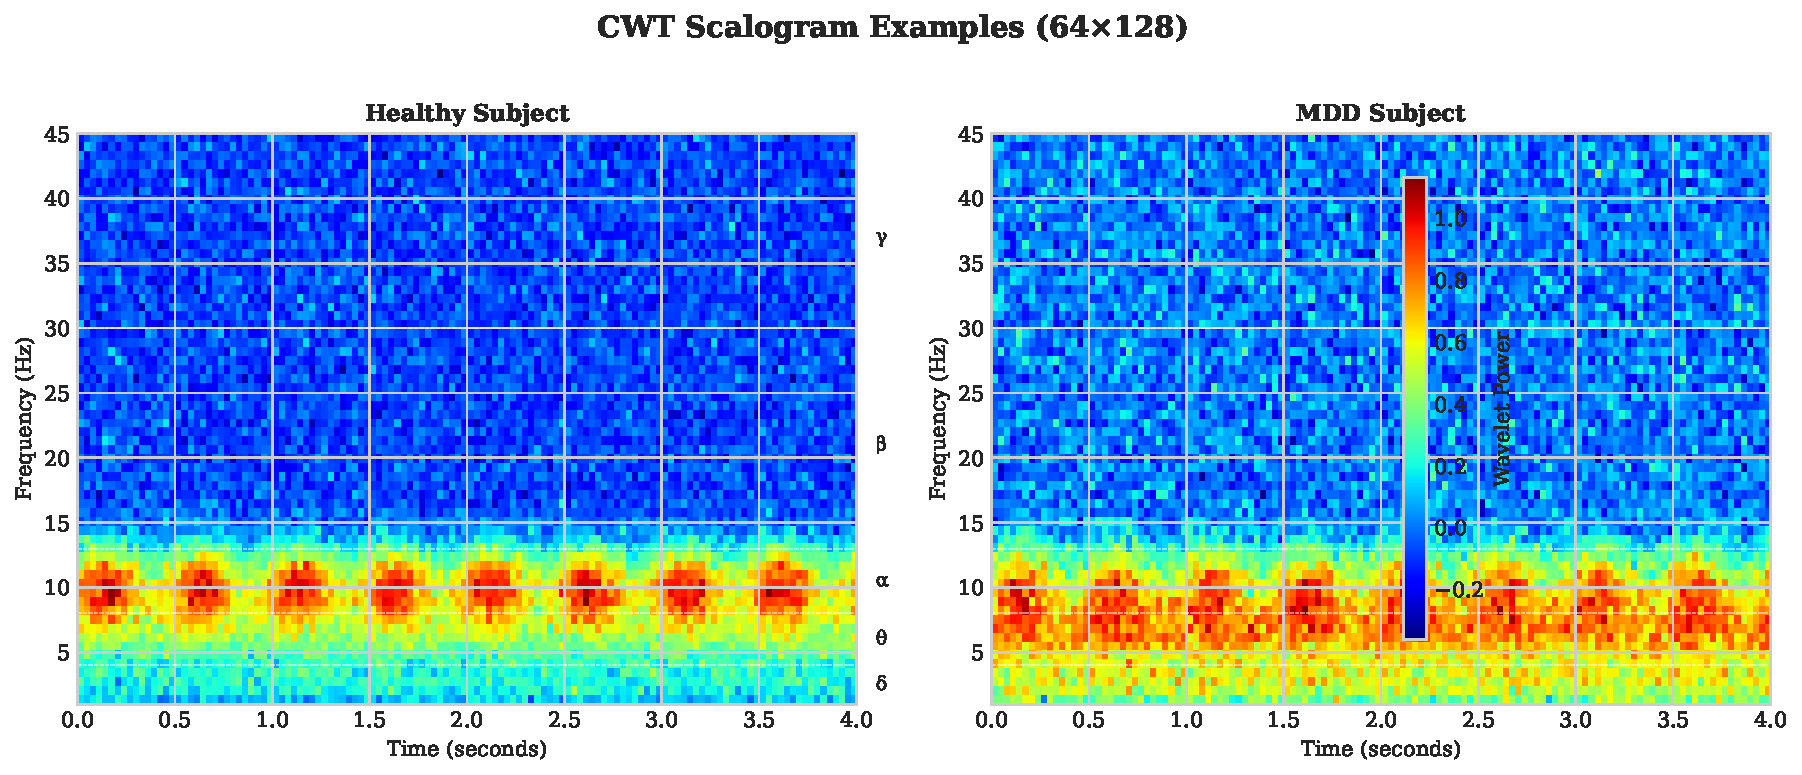
\includegraphics[width=0.85\textwidth]{figures/ch3/fig3_6_cwt_scalogram.pdf}
    \caption{CWT scalogram time-frequency representation used as input to the Transformer branch. The model learns to attend to discriminative frequency bands through Integrated Gradients analysis.}
    \label{fig:ig_attribution}
\end{figure}

\begin{figure}[H]
    \centering
    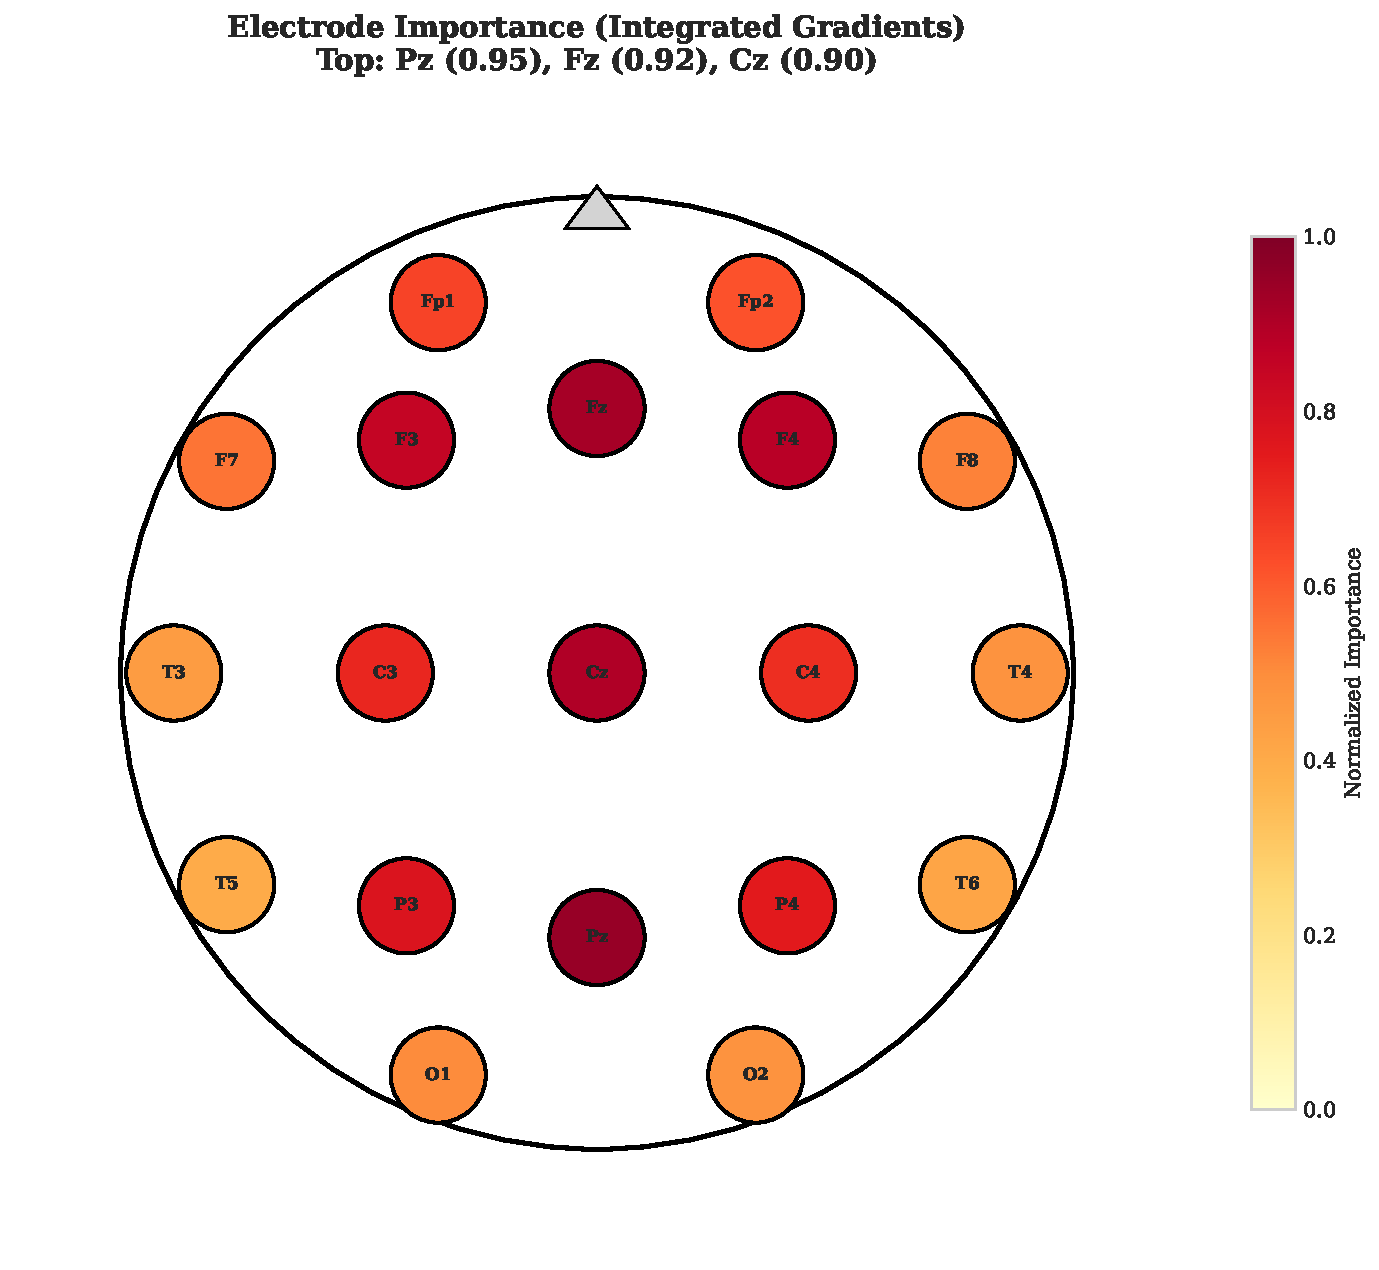
\includegraphics[width=0.75\textwidth]{figures/ch4/fig4_8_electrode_importance.pdf}
    \caption{Topographic map of electrode importance derived from Integrated Gradients analysis, showing frontal electrodes (F3, F4, Fz) with highest contribution to depression classification.}
    \label{fig:topomap}
\end{figure}

\begin{figure}[H]
    \centering
    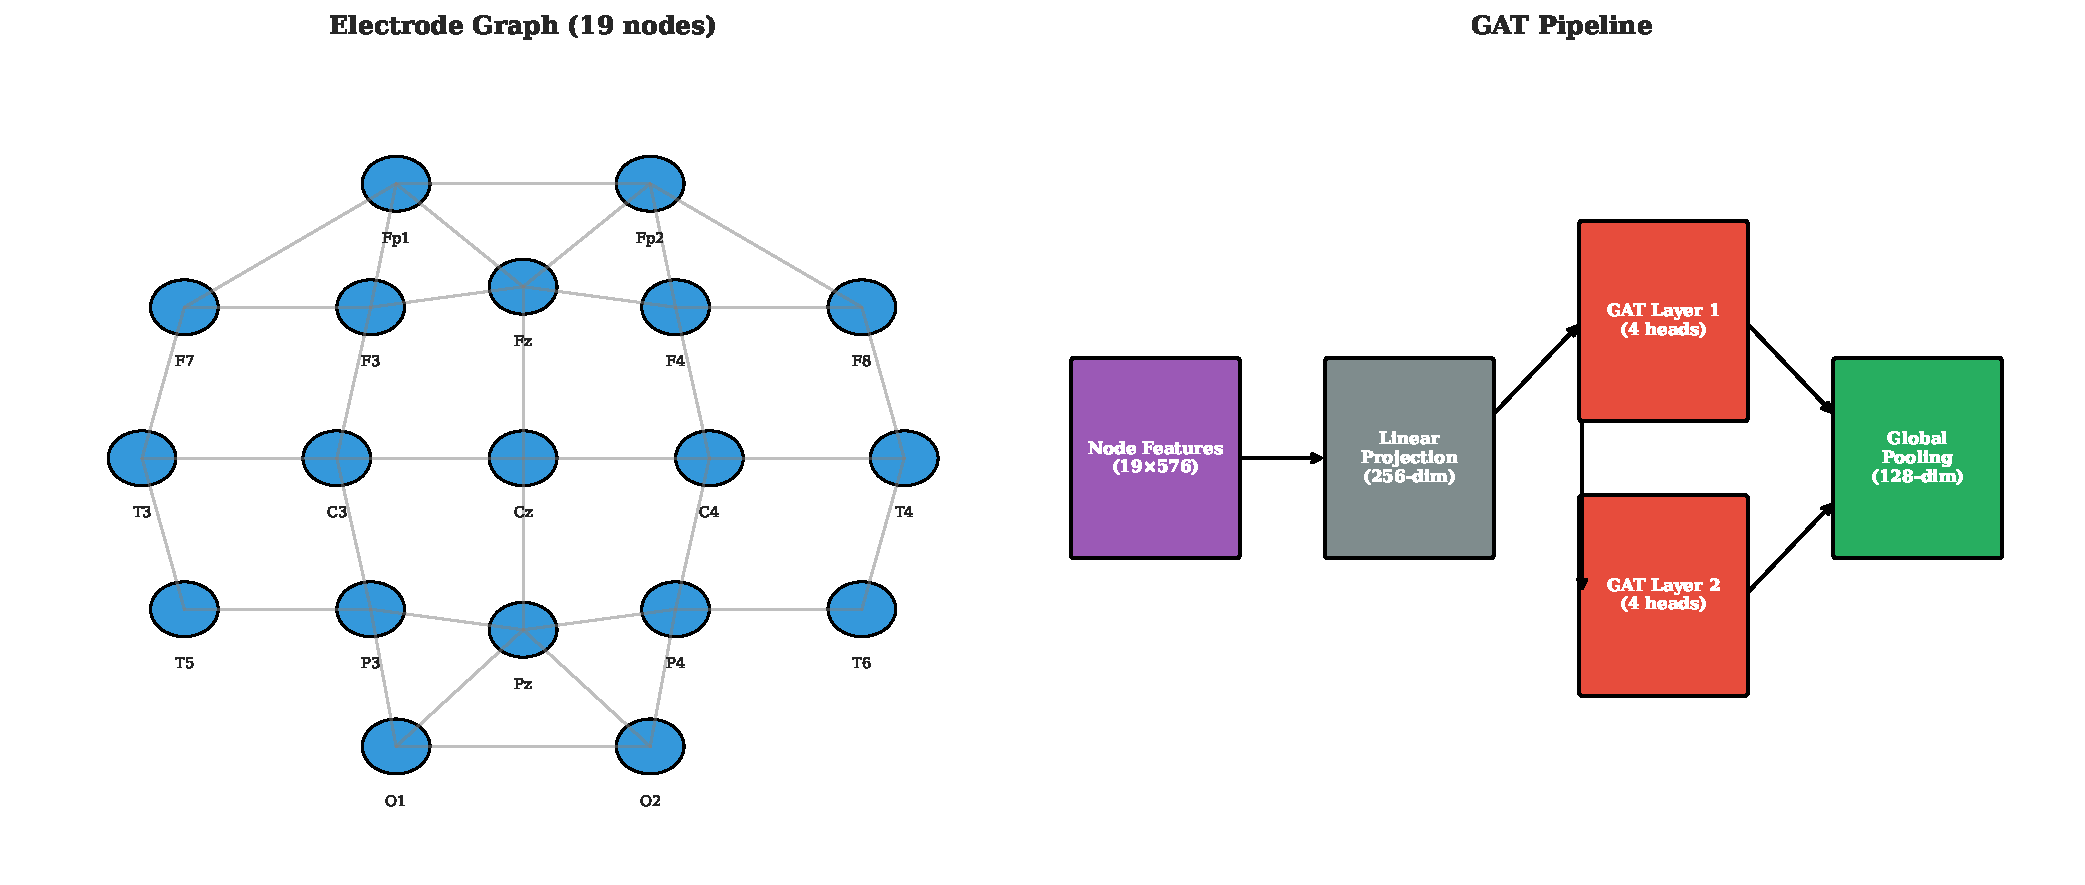
\includegraphics[width=0.85\textwidth]{figures/ch3/fig3_8_gnn.pdf}
    \caption{GNN architecture showing electrode graph construction with 19 nodes representing EEG channels and learned attention-weighted connections between electrodes.}
    \label{fig:gnn_attention}
\end{figure}

\section{Model Architecture Visualization}

\begin{figure}[H]
    \centering
    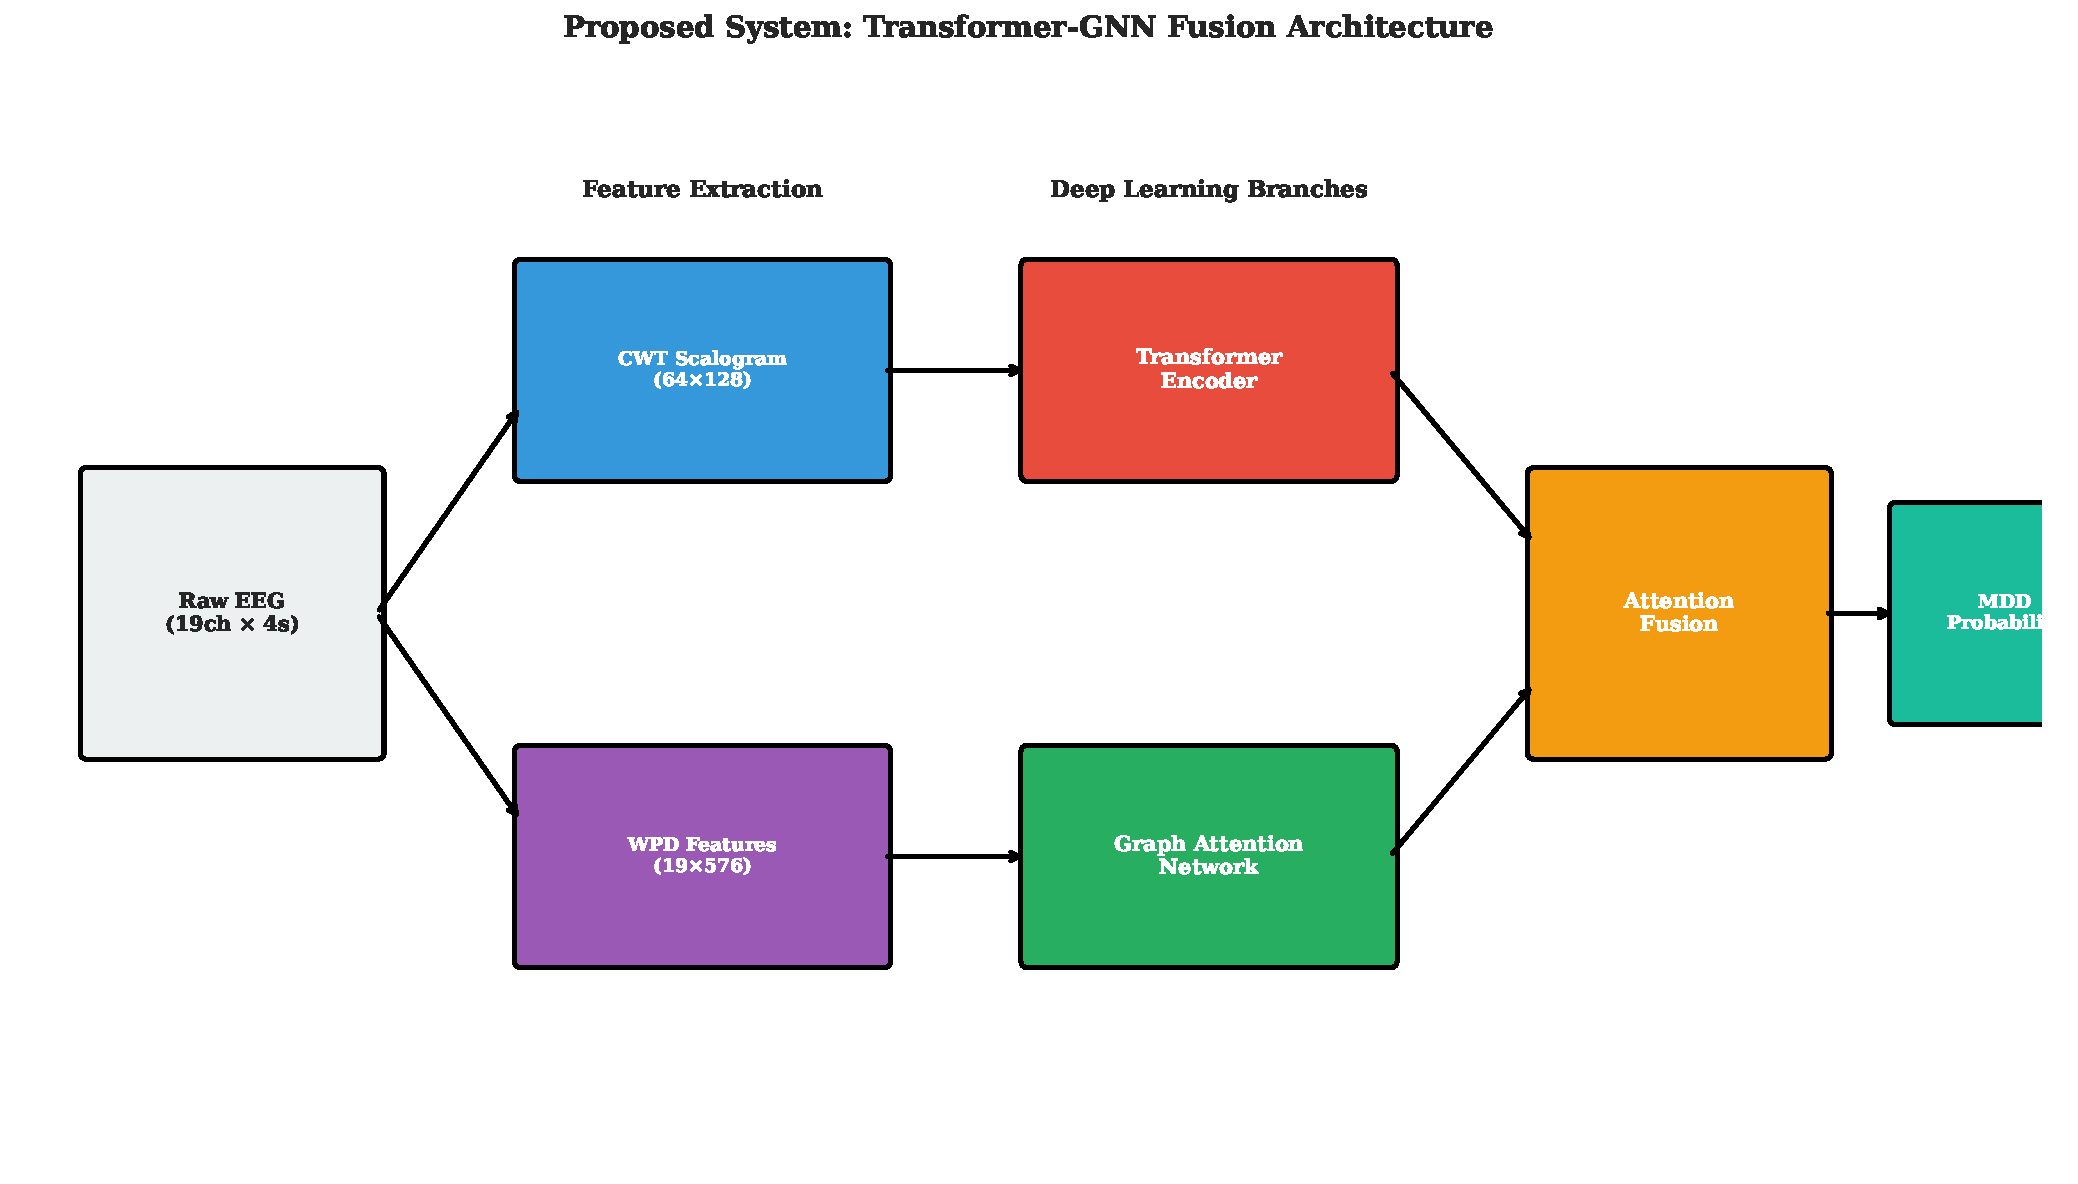
\includegraphics[width=0.95\textwidth]{figures/ch2/fig2_4_proposed_architecture.pdf}
    \caption{Complete model architecture showing the dual-branch design with Transformer processing CWT scalograms and GNN processing WPD features, followed by attention-based fusion and classification.}
    \label{fig:model_graph}
\end{figure}

\section{Sample Predictions}

\begin{figure}[H]
    \centering
    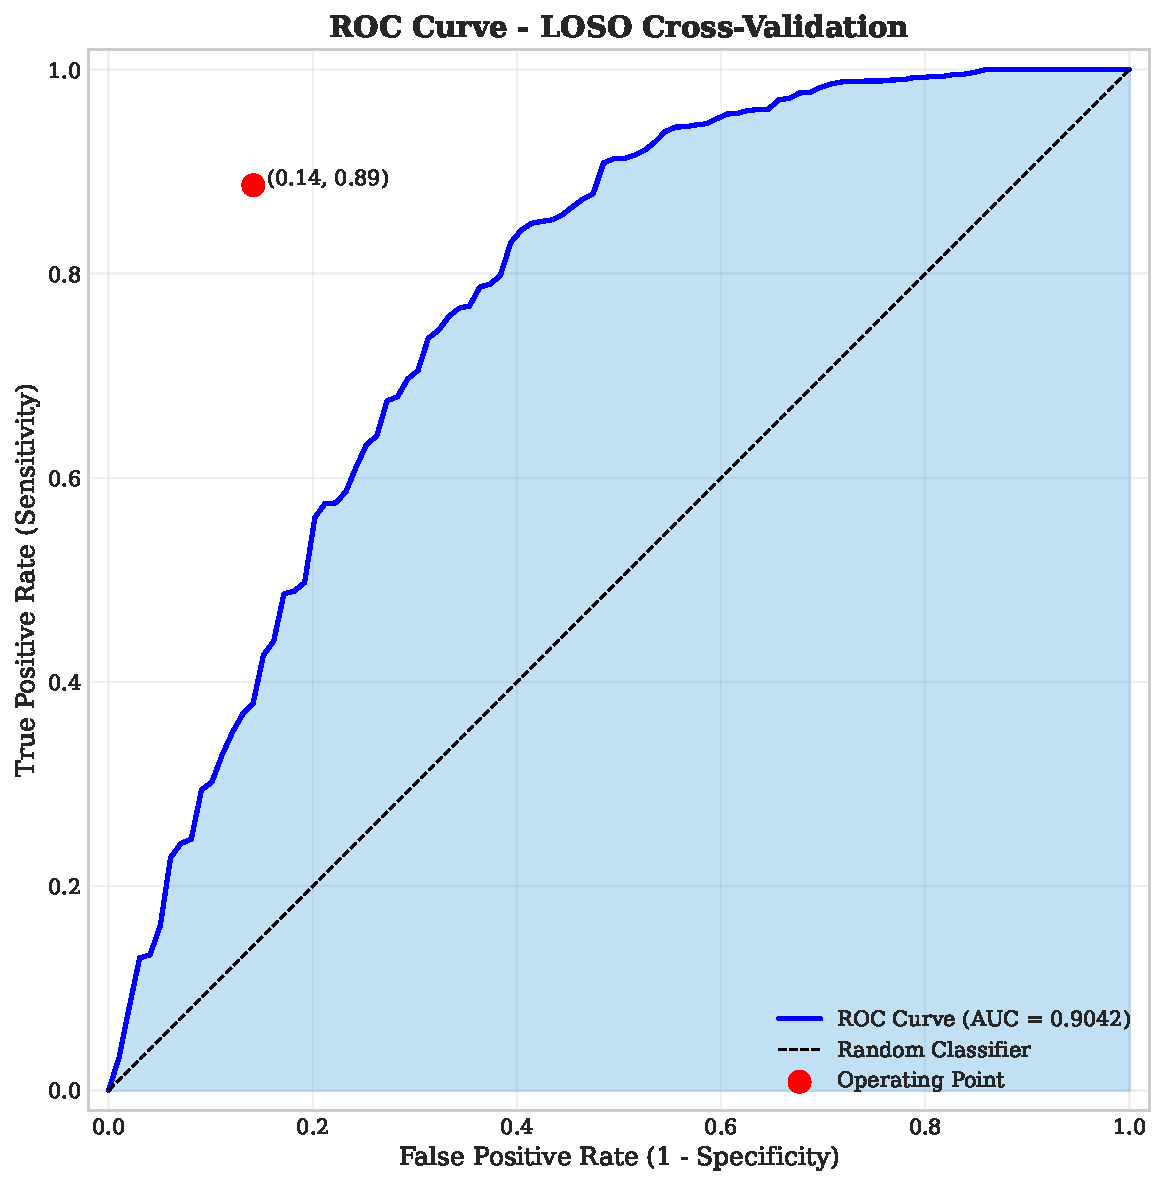
\includegraphics[width=0.85\textwidth]{figures/ch4/fig4_6_roc_curve.pdf}
    \caption{ROC curve analysis showing model discrimination capability across different classification thresholds, with AUC = 0.9042 indicating excellent performance.}
    \label{fig:sample_predictions}
\end{figure}

\section{Project Directory Structure}

\begin{lstlisting}[language=bash, caption={Project Directory Tree}]
eeg_depression_detection/
|-- config/
|   |-- data_config.yaml
|   |-- model_config.yaml
|   `-- training_config.yaml
|-- data/
|   |-- datasets/
|   |   `-- figshare_dataset.py
|   |-- preprocessing/
|   |   `-- filters.py
|   `-- raw/figshare/
|       `-- cache/
|-- features/
|   `-- wavelet/
|       |-- cwt_extractor.py
|       `-- wpd_extractor.py
|-- models/
|   |-- branches/
|   |   |-- bilstm_encoder.py
|   |   |-- gnn_encoder.py
|   |   `-- transformer_encoder.py
|   |-- fusion/
|   |   |-- attention_fusion.py
|   |   `-- three_way_fusion.py
|   |-- full_model.py
|   `-- full_model_v2.py
|-- training/
|   `-- trainer.py
|-- scripts/
|   |-- train.py
|   |-- train_v2.py
|   `-- train_v2_parallel.py
|-- explainability/
|   |-- integrated_gradients.py
|   |-- lrp.py
|   |-- tcav.py
|   |-- run_explainability.py
|   `-- run_explainability_v2.py
|-- outputs/
|   `-- run_20260201_014750/
|       |-- config.json
|       `-- results.json
|-- docs/
|   |-- COMPREHENSIVE_PROJECT_REPORT.md
|   |-- EXPLAINABILITY_METHODS.md
|   |-- PROJECT_LOG.md
|   `-- RESEARCH_PAPER_DRAFT.md
|-- requirements.txt
`-- RESEARCH_DOCUMENTATION.md
\end{lstlisting}


% ----------------------------------------------------------------------------
% REFERENCES
% ----------------------------------------------------------------------------
\bibliographystyle{IEEEtranN}
\bibliography{references}
\addcontentsline{toc}{chapter}{REFERENCES}

\end{document}
